\documentclass[11pt,aspectratio=1610]{beamer}
\usetheme{default}
\usepackage[utf8]{inputenc}
\usepackage[T1]{fontenc}
\usepackage{hyperref}
\usepackage{multimedia}
\usepackage{media9}
\usepackage{animate}
% \usepackage{subfig}
\usepackage[font=scriptsize]{caption}
\usepackage[font=scriptsize]{subcaption}
\usepackage{appendixnumberbeamer}

\usepackage[
    backend=biber,
    style=numeric,
    natbib=true,
    url=false, 
    sorting=none,
    doi=true,
    eprint=false
]{biblatex}
\addbibresource{Biblio.bib}

\usepackage[tensorialbold]{userCommands}
\usepackage[babel=true,kerning=true]{microtype}
\usepackage{amsmath}
\usepackage{amsfonts}
\usepackage{amssymb}
\usepackage{pifont}
\usepackage{mathrsfs}
\usepackage{graphicx}
\usepackage{wasysym}

\usepackage{fancybox}
\usepackage{textcomp}
\usepackage{multicol}
\usepackage{xcolor}
\usepackage{lmodern}
\usepackage{tkz-kiviat}
\RequirePackage{tikz}
\usetikzlibrary{patterns} 
\usetikzlibrary{shapes}
\usetikzlibrary{snakes}
\usetikzlibrary{pgfplots.groupplots}
\usetikzlibrary{spy,backgrounds}
\usetikzlibrary{decorations.markings}
\usetikzlibrary{arrows.meta}
\usetikzlibrary{external} % avoid the systematic compilation of figures
\usepackage{pgfplots}
% \usepackage{pgfplotsthemetol}
\tikzexternalize[prefix=external/]
\pgfplotsset{compat=newest,
  grid=both,
  every axis/.append style={font=\scriptsize},
  tick label style={font=\scriptsize},
  label style={font=\scriptsize},
  title style={font=\scriptsize},
  legend style={font=\footnotesize},
  legend cell align={left},
  yticklabel style={/pgf/number format/fixed},
  % define user colormap
  colormap={tol}{[1cm] rgb255(0cm)=(120,28,129) rgb255(1cm)=(63,96,174) rgb255(2cm)=(83,158,182) rgb255(3cm)=(109,179,136) rgb255(4cm)=(202,184,67) rgb255(5cm)=(231,133,50) rgb255(6cm)=(217,33,32)}
}

\newcommand{\xmark}{\color{Red}\ding{55}}
\newcommand{\cmark}{\color{Green}\ding{51}}

%% User colors
\definecolor{Purple}{RGB}{120,28,129}
\definecolor{Blue}{RGB}{63,96,174}
\definecolor{Duck}{RGB}{83,158,182}
\definecolor{Green}{RGB}{109,179,136}
\definecolor{Yellow}{RGB}{202,184,67}
\definecolor{Orange}{RGB}{231,133,50}
\definecolor{Red}{RGB}{217,33,32}

\usefonttheme{professionalfonts}

\usetheme[progressbar=foot,
subsectionpage=none,
sectionpage=progressbar,
block=transparent%fill
]{metropolis}

\useoutertheme{Headinfoline}
\setbeamertemplate{section in toc}{{\inserttocsectionnumber.}~\inserttocsection    \vspace{-.05\baselineskip}}
% \setbeamertemplate{subsection in toc}{{\inserttocsubsectionnumber.}~\inserttocsubsection    \vspace{-.1\baselineskip}}

\setbeamerfont{section in toc}{size=\normalsize,series=\bfseries}
\setbeamerfont{subsection in toc}{size=\footnotesize}
    
%% CHANGE COLOR SETTINGS
\definecolor{mDarkBrown}{HTML}{604c38}
\definecolor{mDarkTeal}{HTML}{23373b}
\definecolor{mLightBrown}{HTML}{EB811B}
\definecolor{mLightGreen}{HTML}{14B03D}
\definecolor{CNBlue}{RGB}{16,38,72}
\definecolor{CNYellow}{RGB}{250,182,0}

%% fg= ; bg= background 
\setbeamercolor{normal text}{ fg= CNBlue!90 , bg= black!2 }
%\setbeamercolor{alerted text}{ fg=mDarkTeal  }
%\setbeamercolor{exemple text}{ fg=mDarkTeal  }



\setbeamerfont{bibliography entry author}{size=\scriptsize,series=\normalfont}
\setbeamerfont{bibliography entry title}{size=\scriptsize,series=\bfseries}
\setbeamerfont{bibliography entry location}{size=\scriptsize, series=\normalfont}
\setbeamerfont{standout}{size=\Large,series=\bfseries}
%%%%%%%%%%caracterisation du document %---------------------------------------------------------------------
\hypersetup{
	pdftitle    = {Formulation of the DGMPM},
	pdfsubject  = {Ph.D thesis defense- December 2018},
	linkcolor    = red,
	pdfauthor   = {Adrien Renaud},
	pdfkeywords = {numerical simulation, hyperbolic problems, discontinuous Galerkin}
	colorlinks=true,
	linkcolor=black,
	citecolor=blue,
	urlcolor=blue
}



%%-------------- Construction de la page de presentation -------------------------------------------------------
\title[The Discontinuous Galerkin Material Point Method]
{\Large\bf  {The Discontinuous Galerkin Material Point Method: \\application to hyperbolic problems in solid mechanics}}

\date[]{
	\footnotesize{PhD thesis defense} --
	December 14th 2018 \\ \hspace*{7.cm}\includegraphics[trim = 0cm 4cm 0cm 0cm, clip,scale=0.1]{Logo_GEM.pdf} \hspace*{2.cm}\includegraphics[scale=0.25]{Logo_ECN.pdf}}%\logo{ \includegraphics[trim = 0cm 4cm 0cm 0cm, clip,scale=0.1]{Logo_GEM.pdf} \hspace*{2.cm}\includegraphics[scale=0.25]{Logo_ECN.pdf}}
\author{A. Renaud \\ Supervisors: T. Heuz\'e, L. Stainier} 


%------------------------------------------------------------------------

\setbeamertemplate{bibliography item}{\insertbiblabel}

%% Baptist's beamer clock

\newcommand{\myBeamerClock}[2]{
  % #1 is the radius of the clock
  % #2 is the vertical shift for inline placement
  % #3 is the number of current frame
  % #4 is the total number of frames
  \tikz[baseline=#2]{
    \filldraw (0,0) -- (0,#1) arc (90:(90-(\insertframenumber/\inserttotalframenumber)*360):#1);
    \draw (0,0) circle (#1);
  }
}

\newcommand{\footnoteCite}[1]{
  {\tiny 
  \begin{flushleft}
    \foreach \x in {#1}{\cite{\x}  \fullcite{\x}\\}
  \end{flushleft}
}
}
  

% \defbeamertemplate*{footline}{mytheme}{%
%   \usebeamerfont{page number in head/foot}\begin{beamercolorbox}[sep=1.em]{} \hfill  \insertframenumber{}/\inserttotalframenumber{} 
%  \end{beamercolorbox}
% }
%% OR with baptiste's clock
\defbeamertemplate*{footline}{mytheme}{%
  \usebeamerfont{page number in head/foot}\begin{beamercolorbox}[sep=1.em]{} \hfill  \insertframenumber{} \tikzexternaldisable \myBeamerClock{1ex}{-1ex} \tikzexternalenable
 \end{beamercolorbox}
}


%% Arrows along paths in plastic waves study
\tikzset{
  arrows along my path/.style={
    postaction={
      decorate,
      decoration={
        markings,
        mark=between positions 0.03 and 1 step 24pt with {\arrow{Stealth[length=8pt]}},
   }}}}
%% ----------------------------------

\pgfplotsset{select coords between index/.style 2 args={
    x filter/.code={
        \ifnum\coordindex<#1\def\pgfmathresult{}\fi
        \ifnum\coordindex>#2\def\pgfmathresult{}\fi
    }
  }}


\makeatletter
\AtBeginPart{%
  \beamer@tocsectionnumber=0\relax
  \setcounter{section}{0}
  \frame[plain,noframenumbering]{\partpage}%
}
\makeatother

%% Enable to use nameref with part
\makeatletter
\let\oldpart\part
\def\part#1{\def\@currentlabelname{#1}\oldpart{#1}}
\makeatother

%% New command to remove headline
\makeatletter
\newenvironment{withoutheadline}{
  \setbeamertemplate{headline}[default]
  \def\beamer@entrycode{\vspace*{-\headheight}}
}{}
\makeatother

%\pgfkeys{/kiviat/label style/.style={align=center,anchor=180+360/\tkz@kiv@radial*\rang}}

\begin{document}

\begin{frame}[plain]
  \maketitle
\end{frame}




\begin{frame}{From physics to the mathematical model}
  % Concerned with solid dynamics problems such as Impact or crash-proof design.
  % in the first case, one wants to ensure that a structure undegoing dynamic loadings remains usable while in the latter, it is expected to dissipate as much energy as possible so that the passengers are safe
  
  % On the other hand, high-speed forming techniques such as electromagnetic forming also involve dynamic loadings

  % At last, another challenging field of dynamics is the reliability of structures to earthquakes
  % Here is depicted the mass damper of the Taipei 101 tower which design was possible thanks to a good understanding of the physics.
  \vspace{-0.6cm}
  \begin{overprint}
    \onslide<1>
    \begin{columns}
      \begin{column}{0.45\textwidth}
        \begin{block}{Solid dynamics problems}
          \begin{itemize}
          \item[] \textbf{Impact; Crash-proof design}
          \item[] High-speed forming
          \item[] Earthquake reliability of structures 
          \end{itemize}
        \end{block}
      \end{column}
      
      \begin{column}{0.55\textwidth}
      \end{column}
    \end{columns}
    
    \begin{figure}[ht]
      \centering
      \subcaptionbox{Bird strike on aircrafts}{\includegraphics[height=0.3\paperheight]{section1/pictures/birdstrike.jpg}}
      \subcaptionbox{Glasgow Museum of Transport}{\includegraphics[height=0.3\paperheight]{section1/pictures/crash2.jpg}}
    \end{figure}
    
    \onslide<2>
    \begin{columns}
      \begin{column}{0.45\textwidth}
        \begin{block}{Solid dynamics problems}
          \begin{itemize}
          \item[] Impact; Crash-proof design
          \item[] \textbf{High-speed forming}
          \item[] Earthquake reliability of structures 
          \end{itemize}
        \end{block}
      \end{column}
      
      \begin{column}{0.55\textwidth}
      \end{column}
    \end{columns}
    \centering
      \movie[height = 0.35\paperheight,width=0.25\linewidth,loop,poster,autostart]{}{%
      section1/animation/output3.mp4}\\
    \scriptsize Electromagnetic forming \cite{Guillaume}
    \footnoteCite{Guillaume}
    
    \onslide<3>
    \begin{columns}
      \begin{column}{0.45\textwidth}
        \begin{block}{Solid dynamics problems}
          \begin{itemize}
          \item[] Impact; Crash-proof design
          \item[] High-speed forming
          \item[] \textbf{Earthquake reliability of structures}
          \end{itemize}
        \end{block}
      \end{column}
      
      \begin{column}{0.55\textwidth}
      \end{column}
    \end{columns}

    \centering
    \includegraphics[scale=0.15]{section1/pictures/TaipeiTower.png} \quad
    \includegraphics[scale=0.08]{section1/pictures/MassDamper.jpg}\\
    \scriptsize Taipei 101 mass damper

    \onslide<4>
    \begin{columns}
      \begin{column}{0.45\textwidth}
        \begin{block}{Solid dynamics problems}
          \begin{itemize}
          \item[] Impact; Crash-proof design
          \item[] High-speed forming
          \item[] Earthquake reliability of structures 
          \end{itemize}
        \end{block}
      \end{column}
      
      %% The governing equations allowing to mathematically model those physical phenomena are composed of Conservation laws and constitutive equations, which can be written as a hyperbolic system
      %% Even though models can be built, the complex geometries, waves propagating in solids and the possibly finite deformations make in general the exact solution not possible.
      %% As a result, the numerical simulation based on space and time approximations becomes helpfull
      \begin{column}{0.55\textwidth}
        \begin{block}{Partial differential equations}
          \begin{equation*}
            \Rightarrow \left\lvert
              \begin{aligned}
                & \text{Conservation laws} \\
                & \text{Constitutive equations} 
              \end{aligned}
            \right. = \textbf{Hyperbolic system}
            % Préciser les équations dans le dévelopement de la DGMPM
          \end{equation*}
        \end{block}
      \end{column}
    \end{columns}
    
    \begin{block}{Difficulties for the solution of hyperbolic equations:}
      \begin{itemize}
      \item complex geometries
      \item waves propagating/interacting in solids \cite{Wang}
      \item finite deformations
      \end{itemize}
    \end{block}
    \textbf{$\Rightarrow$ Resort to numerical simulation:} space and time discretization techniques
    \footnoteCite{Wang}
  \end{overprint}
  
\end{frame}

\begin{frame}{Suitability of some explicit methods}
  %% Among the big stars of existing numerical methods, the FEM
  \begin{block}{The Finite Element Method \cite{Belytschko}}
    \vskip 4pt
    \begin{overprint}
      \onslide<1>
      \begin{columns}
        \begin{footnotesize}
          \begin{column}{0.5\textwidth}
            \begin{itemize}
            \item[] Mesh-based space discretization
            \item[] Weak form of balance equation
            \end{itemize}
          \end{column}
          \begin{column}{0.5\textwidth} 
            \begin{itemize}
            \item[] Polynomial approximation
            \item[] Gauss points constitutive update
            \end{itemize}
          \end{column}
        \end{footnotesize}
      \end{columns}
      \onslide<2>
      \begin{columns}
        \begin{footnotesize}
          \begin{column}{0.5\textwidth}
            \begin{itemize}
            \item[] Mesh-based space discretization
            \item[] Weak form of balance equation
            \end{itemize}
          \end{column}
          \begin{column}{0.5\textwidth} 
            \begin{itemize}
            \item[] Polynomial approximation
            \item[] Gauss points constitutive update
            \end{itemize}
          \end{column}
        \end{footnotesize}
      \end{columns}
      \vskip -10pt
      \begin{columns}
        \begin{column}{0.48\textwidth}
          \begin{block}{\footnotesize Lagrangian formulation}
            \centering
            \begin{tikzpicture}[scale=0.4]
              \tkzKiviatDiagram[lattice=4,
              label style/.append style={font=\tiny},radial  style/.style ={->},lattice style/.style ={white,opacity=0}]{CFL,Non-diffusive,Mesh robustness,Non-oscillating,High-order}
              \tkzKiviatLine[thick,color = black!50](4,4,4,4,4)
              
              \tkzKiviatLine[thick,color = Blue,fill= Blue,opacity=.7](4,4,1,1,3)
            \end{tikzpicture}
          \end{block}
        \end{column}
        \begin{column}{0.48\textwidth}
          % \begin{block}{\footnotesize Eulerian formulation}
          %   \centering
          %   \begin{tikzpicture}[scale=0.4]
          %     \tkzKiviatDiagram[lattice=4,
          %     label style/.append style={font=\tiny},radial  style/.style ={->},lattice style/.style ={white,opacity=0}]{CFL,Non-diffusive,Distortion-free,Non-oscillating,High-order}
          %     \tkzKiviatLine[thick,color = black!50](4,4,4,4,4)
              
          %     \tkzKiviatLine[thick,color = Blue,fill= Blue,opacity=.7](4,2,4,1,3)
          %   \end{tikzpicture}
          % \end{block}
        \end{column}
      \end{columns}
    \end{overprint}
  \end{block}
\footnoteCite{Belytschko}
\end{frame}

%% Pas forcément mettre en avant le tangling
%% Approches Lagrangiennes FVM qui ont des di
%% Citer Maire le papier de 2006 sur la définition de la vitesse nodale (similaire au DG puisque v est discontinue) -> pas tant mesh entanglement que mesh update issues (le second étant valable même en total lagrangian)
%% Virer l'Eulérien; mettre mesh drawbacks; citer le cas échéant; et préciser à l'oral les mesh drawbacks: pour FVM, il s'agit de bouger le maillage avec un champ de vitesse discontinu
\begin{frame}{Suitability of some explicit methods}
  \begin{block}{The Finite Volume Method \cite{Leveque}}%\cite{Haider_FVM} for total Lagrangian
    \vspace{-0.2cm}
    \begin{overprint}
      \onslide<1>
      \vspace{-0.2cm}
      \begin{columns}
        \begin{footnotesize}
          \begin{column}{0.4\textwidth}
            \begin{itemize}
            \item[] Mesh-based space discretization
            \item[] Conservation laws
            \end{itemize}
        \end{column}
        \begin{column}{0.6\textwidth}
            \begin{itemize}
            \item[] Cell-wise approximation and constitutive update
            \item[] Intercell fluxes -- characteristic structure \cite{Godunov_method}
            \end{itemize}
          \end{column}
        \end{footnotesize}
      \end{columns}
      \vspace{3.65cm}
      \footnoteCite{Leveque,Godunov_method}
      \onslide<2>
      \vspace{-0.2cm}
      \begin{columns}
        \begin{footnotesize}
          \begin{column}{0.4\textwidth}
            \begin{itemize}
            \item[] Mesh-based space discretization
            \item[] Conservation laws
            \end{itemize}
          \end{column}
          \begin{column}{0.6\textwidth}
            \begin{itemize}
            \item[] Cell-wise approximation and constitutive update
            \item[] Intercell fluxes -- characteristic structure \cite{Godunov_method}
            \end{itemize}
          \end{column}
        \end{footnotesize}
      \end{columns}
      \vskip -10pt
      \begin{columns}
        \begin{column}{0.48\textwidth}
          \begin{block}{\footnotesize Lagrangian formulation \cite{Haider_FVM}} %[Haider]?}
            \centering
            \begin{tikzpicture}[scale=0.4]
              \tkzKiviatDiagram[lattice=4,
              label style/.append style={font=\tiny},radial  style/.style ={->},lattice style/.style ={white,opacity=0}]{CFL,Non-diffusive, Mesh robustness,Non-oscillating,High-order}
              \tkzKiviatLine[thick,color = black!50](4,4,4,4,4)
              
              \tkzKiviatLine[thick,color = Red,fill= Red,opacity=.7](4,4,1,4,1)
            \end{tikzpicture}
          \end{block}
        \end{column}
        \begin{column}{0.48\textwidth}
          % \begin{block}{\footnotesize Eulerian formulation}
          %   \centering
          %   \begin{tikzpicture}[scale=0.4]
          %     \tkzKiviatDiagram[lattice=4,
          %     label style/.append style={font=\tiny},radial  style/.style ={->},lattice style/.style ={white,opacity=0}]{CFL,Non-diffusive,Distortion-free,Non-oscillating,High-order}
          %     \tkzKiviatLine[thick,color = black!50](4,4,4,4,4)
              
          %     \tkzKiviatLine[thick,color = Red,fill= Red,opacity=.7](4,2,4,4,1)
          %   \end{tikzpicture}
          % \end{block}
        \end{column}
      \end{columns}
      \vspace{-0.2cm}
      \footnoteCite{Leveque,Godunov_method,Haider_FVM}
    \end{overprint}
  \end{block}
  %compatibility between the two configurations based on Eulerian and Lagrangian coordinates
  
  
\end{frame}


\begin{frame}{Suitability of some explicit methods}
  \begin{block}{The Discontinuous Galerkin Finite Element Method \cite{Cockburn}}
    \vspace{-0.2cm}
    \begin{overprint}
      \onslide<1>
      \vspace{-0.2cm}
      \begin{columns}
        \begin{footnotesize}
          \begin{column}{0.4\textwidth}
            \begin{itemize}
            \item[] Mesh-based space discretization
            \item[] Cell-wise weak form \cite{NeutronDG}
            \end{itemize}
          \end{column}
          \begin{column}{0.6\textwidth}
            \begin{itemize}
            \item[] Gauss points constitutive update
            \item[] Intercell fluxes -- characteristic structure
            \end{itemize}
          \end{column}
        \end{footnotesize}
      \end{columns}
      \vspace{3.65cm}
      \footnoteCite{Cockburn,NeutronDG}
      \onslide<2>
      \vspace{-0.2cm}
      \begin{columns}
        \begin{footnotesize}
          \begin{column}{0.4\textwidth}
            \begin{itemize}
            \item[] Mesh-based space discretization
            \item[] Cell-wise weak form \cite{NeutronDG}
            \end{itemize}
          \end{column}
          \begin{column}{0.6\textwidth}
            \begin{itemize}
            \item[] Gauss points constitutive update
            \item[] Intercell fluxes -- characteristic structure
            \end{itemize}
          \end{column}
        \end{footnotesize}
      \end{columns}
      \vskip -10pt
      \begin{columns}
        \begin{column}{0.48\textwidth}
          \begin{block}{\footnotesize Lagrangian formulation \cite{LagrangianDG_thesis}}
            \centering
            \begin{tikzpicture}[scale=0.4]
              \tkzKiviatDiagram[lattice=4,
              label style/.append style={font=\tiny},radial  style/.style ={->},lattice style/.style ={white,opacity=0}]{CFL,Non-diffusive,Mesh robustness,Non-oscillating,High-order}
              \tkzKiviatLine[thick,color = black!50](4,4,4,4,4)
              
              \tkzKiviatLine[thick,color = Purple,fill= Purple,opacity=.7](1,4,1,4,4)
            \end{tikzpicture}
          \end{block}
        \end{column}
        \begin{column}{0.48\textwidth}
          % \begin{block}{\footnotesize Eulerian formulation (check diffusion)}
          %   \centering
          %   \begin{tikzpicture}[scale=0.4]
          %     \tkzKiviatDiagram[lattice=4,
          %     label style/.append style={font=\tiny},radial  style/.style ={->},lattice style/.style ={white,opacity=0}]{CFL,Non-diffusive,Mesh robustness,Non-oscillating,High-order}
          %     \tkzKiviatLine[thick,color = black!50](4,4,4,4,4)
              
          %     \tkzKiviatLine[thick,color = Purple,fill= Purple,opacity=.7](1,2,4,4,4)
          %   \end{tikzpicture}
          % \end{block}
        \end{column}
      \end{columns}
      \vspace{-0.2cm}
      \footnoteCite{Cockburn,NeutronDG,LagrangianDG_thesis}
    \end{overprint}
  \end{block}
\end{frame}



%% OLD VERSION == ONE SLIDE
% \begin{frame}{Suitability of some Lagrangian explicit methods}
%   \begin{columns}
%     \begin{column}{0.3\textwidth}
%       \begin{block}{\footnotesize Finite Element Method \cite{Belytschko}}
%         \begin{tikzpicture}[scale=0.5]
%           \tkzKiviatDiagram[lattice=4,
%           label style/.append style={font=\tiny},radial  style/.style ={->},lattice style/.style ={white,opacity=0}]{CFL,Non-diffusive,Mesh robustness,Non-oscillating,High-order}
%           \tkzKiviatLine[thick,color = black!50](4,4,4,4,4)
          
%           \tkzKiviatLine[thick,color = Blue,fill= Blue,opacity=.7](4,4,1,1,3)
%         \end{tikzpicture}
%       \end{block}
%     \end{column}
%     \begin{column}{0.3\textwidth}
%       \begin{block}{\footnotesize Finite Volume Method \cite{Leveque}}
%         \begin{tikzpicture}[scale=0.5]
%           \tkzKiviatDiagram[lattice=4,
%           label style/.append style={font=\tiny},radial  style/.style ={->},lattice style/.style ={white,opacity=0}]{CFL,Non-diffusive,Mesh robustness,Non-oscillating,High-order}
%           \tkzKiviatLine[thick,color = black!50](4,4,4,4,4)
          
%           \tkzKiviatLine[thick,color = Red,fill= Red,opacity=.7](4,4,1,4,1)
%         \end{tikzpicture}
%       \end{block}
%     \end{column}
%     \begin{column}{0.33\textwidth}
%       \begin{block}{\footnotesize Discontinuous Galerkin FEM \cite{Cockburn}}
%         \begin{tikzpicture}[scale=0.5]
%           \tkzKiviatDiagram[lattice=4,
%           label style/.append style={font=\tiny},radial  style/.style ={->},lattice style/.style ={white,opacity=0}]{CFL,Non-diffusive,Mesh robustness,Non-oscillating,High-order}
%           \tkzKiviatLine[thick,color = black!50](4,4,4,4,4)
          
%           \tkzKiviatLine[thick,color = Blue!70](4,4,1,1,3)
%           \tkzKiviatLine[thick,color = Red!70](4,4,1,4,1)
%           \tkzKiviatLine[thick,color = Purple,fill= Purple,opacity=.7](2,4,1,4,4)
%         \end{tikzpicture}
%       \end{block}
%     \end{column}
%   \end{columns}
%   \footnoteCite{Belytschko,Leveque,Cockburn}
% \end{frame}

%% It then appears that some difficulties related to the mesh are encourted with all the previous methods. 
%% Mesh-free approaches allow however, to circumvent some of them.
%% In particular, the material point method
\begin{frame}{Mesh-free Lagrangian approaches: The Material Point Method \cite{Sulsky94}}
  \nocite{Sulsky94}
  \begin{columns}
    \begin{column}{0.4\textwidth}
      \begin{block}{\footnotesize Particle-in-cell mapping \cite{PIC}}
       \begin{tikzpicture}[scale=0.5]
          \tkzKiviatDiagram[lattice=4,
          label style/.append style={font=\tiny},radial  style/.style ={->},lattice style/.style ={white,opacity=0}]{CFL,Non-diffusive,Mesh robustness,Non-oscillating,High-order}
          \tkzKiviatLine[thick,color = black!50](4,4,4,4,4)
          
          \tkzKiviatLine[thick,color = Yellow,fill= Yellow,opacity=.7](3,1,4,4,3)
        \end{tikzpicture}
      \end{block}
    \end{column}
    \begin{column}{0.4\textwidth}
      \begin{block}{\footnotesize FLuid Implicit Particle mapping \cite{PIC_Nishiguchi}}
        \begin{tikzpicture}[scale=0.5]
          \tkzKiviatDiagram[lattice=4,
          label style/.append style={font=\tiny},radial  style/.style ={->},lattice style/.style ={white,opacity=0}]{CFL,Non-diffusive,Mesh robustness,Non-oscillating,High-order}
          \tkzKiviatLine[thick,color = black!50](4,4,4,4,4)
          
          \tkzKiviatLine[thick,color = Orange,fill= Orange,opacity=.7](3,3,4,1,3)
        \end{tikzpicture}
      \end{block}
    \end{column}
  \end{columns}
  \footnoteCite{Sulsky94,PIC_Nishiguchi,PIC}
\end{frame}

\begin{frame}
  \metroset{block=fill}
  \begin{block}{Objective 1}
    Capture waves with a Lagrangian description while avoiding mesh-related difficulties \\
    %% Solution proposed, though others exist
    \alert{$\Rightarrow$ Merge the advantages of FEM, FVM and MPM by means of the DG approximation}
  \end{block}
  \metroset{block=transparent}
  \begin{block}{The Discontinuous Galerkin Material Point Method}
    \begin{columns}
      \begin{column}{0.6\textwidth}
        \begin{tikzpicture}[scale=0.5]
          \tkzKiviatDiagram[lattice=4,
          label style/.append style={font=\tiny},radial  style/.style ={->},lattice style/.style ={white,opacity=0}]{CFL,Non-diffusive,Mesh robustness,Non-oscillating,High-order}
          \tkzKiviatLine[thick,color = black!50](4,4,4,4,4)
          
          \tkzKiviatLine[thick,color = Yellow!70](3,1,4,4,3)
          \tkzKiviatLine[thick,color = Orange!70](3,3,4,1,3)
          \tkzKiviatLine[thick,color = Purple!70](1,4,1,4,4)
          \tkzKiviatLine[thick,color = Green,fill= Green,opacity=.7](3,2,4,4,3)
        \end{tikzpicture}
      \end{column}
      \begin{column}{0.4\textwidth}
        \textbf{Ingredients:}
        \begin{itemize}
        \item MPM space discretization
        \item PIC projection of fields
        \item DG approximation
        \end{itemize}
      \end{column}
    \end{columns}
  \end{block}
\end{frame}

\begin{frame}{The simulation is bounded by the model}
  %%
  \begin{block}{Inheritance from fluid dynamics}
    Numerical tools to embed information about the solution in numerical approaches
  \end{block}
  \begin{block}{Point of view adopted: Such numerical tools + robust discretization techniques}
    \begin{itemize}
    \item Provide accurate solutions
    \item Enable a numerical approach to mimic the physical response
    \end{itemize}
  \end{block}
  \begin{block}{Limitations}
    Gaps about some constitutive models (damage, plasticity, thermo-mechanical coupling etc.)
  \end{block}
  \metroset{block=fill}
  \begin{block}{Objective 2}
    Identify the response of two-dimensional elastic-plastic solids to dynamic loading
  \end{block}
\end{frame}



%%% Local Variables:
%%% mode: latex
%%% TeX-master: "../presentation"
%%% End:



\begin{frame}[plain,]
  \begin{columns}
    \begin{column}{0.45\textwidth}
      \begin{block}{Part I: \nameref{part:part1} \insertpart}
        \tableofcontents[part=1,hideallsubsections]
      \end{block}
    \end{column}
    \begin{column}{0.55\textwidth}
      \begin{block}{Part II: \nameref{part:part2}}
        \tableofcontents[part=2,hideallsubsections]
      \end{block}
    \end{column}
  \end{columns}
\end{frame}

\AtBeginSection[]{%
  \begin{frame}[plain,]\frametitle{Outline}\tableofcontents[currentsection,hideallsubsections]\end{frame}}
\part{Development of the DGMPM}

\label{part:part1}




\section{Derivation of the DGMPM}
\subsection{Continuum equations}

\begin{frame}
  \begin{block}{Solid volume $\Omega_0$ bounded by $\partial \Omega$ in the reference configuration}
    \metroset{block=fill}
    % Cartesian coordinates system
    \begin{footnotesize}
      \begin{columns}
        \begin{column}{0.5\textwidth}
          \begin{block}{Finite strain}
            \begin{flalign*}
              \: \rho_0 & \drond{\vect{v}}{t} - \nablav_0 \cdot \tens{\Pi} = \rho_0\vect{b} &\\
              & \drond{\tens{F}}{t} - \nablav_0 \cdot (\vect{v} \otimes \tens{I})= \tens{0} \\
              & \Ucb = \matrice{\rho_0\vect{v} \\ \tens{F}} \: ; \: \Fcb=-\matrice{\tens{\Pi}\\ \vect{v} \otimes \tens{I}}\: ; \: \Scb=\matrice{\rho_0\vect{b} \\ \tens{0}}
            \end{flalign*} 
          \end{block}
        \end{column}
        \begin{column}{0.5\textwidth}
          \begin{block}{Linearized geometrical framework}
            \begin{flalign*}
              \: \rho_0 & \drond{\vect{v}}{t} - \nablav_0 \cdot \tens{\sigma} = \rho_0\vect{b} &\\
              & \drond{\tens{\eps}}{t} - \nablav_0 \cdot \frac{\vect{v} \otimes \tens{I} + \tens{I}\otimes \vect{v}}{2}= \tens{0} \\
              & \Ucb = \matrice{\rho_0\vect{v} \\ \tens{\eps}} \: ; \: \Fcb=-\matrice{\tens{\sigma}\\ \frac{\vect{v} \otimes \tens{I} + \tens{I}\otimes \vect{v}}{2}}\: ; \: \Scb=\matrice{\rho_0\vect{b} \\ \tens{0}}
            \end{flalign*}
          \end{block}
        \end{column}
      \end{columns}
      \pause
      \textbf{\normalsize System of Lagrangian conservation laws \cite{Plohr}:}
      \begin{equation*}
        \drond{\Ucb}{t} + \nablav_0 \cdot \Fcb = \Scb
      \end{equation*}
    \end{footnotesize}
    {\tiny
      \usebibitemtemplate{\color{structure}\insertbiblabel} 
      \usebibliographyblocktemplate{\color{structure}}{\color{black}}{\color{structure!75}}{\color{structure!75}} 
      \begin{thebibliography}{ThomasEM}
      \bibitem[1]{Plohr}
        B.J. Plohr, D.H. Sharp.
        \newblock A conservative Eulerian formulation of the equations for elastic flow
        \newblock {\em Advances in Applied Mathematics (1988)}.
      \end{thebibliography}}
  \end{block}
  
\end{frame}

\begin{frame}
  %% Alternatively by introducing the constitutive equations, one can write the quasi-linear form
  %% Required ??
  \begin{columns}
    \begin{column}{0.5\textwidth}
      \begin{block}{Constitutive models}
        \metroset{block=fill}
        \begin{block}{Finite strains}
          Hyperelasticity: $\dot{\tens{\Pi}} = \Hbb(\tens{F}) : \dot{\tens{F}}$
        \end{block}
        \begin{block}{Linearized geometrical framework}
          Linear elasticity: $\dot{\tens{\sigma}} = \Cbb : \dot{\tens{\eps}}$ \\
          Elasto-viscoplasticity: $\dot{\tens{\sigma}} = \Cbb : (\dot{\tens{\eps}}-\dot{\tens{\eps}^p})$\\
          Elastoplasticity: $\dot{\tens{\sigma}} = \Hbb(\tens{\sigma}) : \dot{\tens{\eps}}$
        \end{block}    
      \end{block}
    \end{column}
    \pause
    \begin{column}{0.5\textwidth}
      \begin{block}{Quasi-linear forms}
        \begin{block}{}
          $\Qcb=\matrice{\tens{\Pi}\\\vect{v}} \rightarrow \drond{\Qcb}{t} + \nablav_0 \cdot \Fcb = \Scb$
        \end{block}
        \begin{block}{}
          % Linear elasticity: $\dot{\tens{\sigma}} = \Cbb : \dot{\tens{\eps}}$ \\
          % Elasto-viscoplasticity: $\dot{\tens{\sigma}} = \Cbb : (\dot{\tens{\eps}}-\dot{\tens{\eps}^p})$\\
          % Elastoplasticity: $\dot{\tens{\sigma}} = \Hbb(\tens{\sigma}) : \dot{\tens{\eps}}$
        \end{block}    
      \end{block}
    \end{column}
  \end{columns}
  
  
\end{frame}

\subsection{Discrete system}
\subsection{Non-homogeneous systems}
\subsection{Interface fluxes}
%%% Local Variables:
%%% mode: latex
%%% TeX-master: "../presentation"
%%% End:



\section{The numerical scheme -- Analysis}
\subsection{Solution scheme}

\begin{frame}{Procedure between $t^n$ and $t^n + \Delta t^n=t^{n+1}$}
  \begin{footnotesize}
    %% Computation of matrices
    \begin{equation*}
      \text{Discrete system: }\alert{M^L_{i}} \frac{\bar{\Ucb}^{i,n+1} - \bar{\Ucb}^{i,n}}{\Delta t^n}  - \alert{K_{ij}^\alpha} \bar{\Fcb}^{j,n}_{\alpha}  + \hat{\Fcb}^{i,n}=  \vect{0}
    \end{equation*}
    \begin{columns}
      \begin{column}{0.4\textwidth}
        \begin{itemize}
        \item[(1)] Computation of matrices $M_i^L$ and $K_{ij}^\alpha$
        \end{itemize}
      \end{column}
      \vrule{}
      \begin{column}{0.6\textwidth}
        \begin{block}{Computation of matrices $M_i^L$ and $K_{ij}^\alpha$}
          \begin{columns}
            \begin{column}{0.3\textwidth}
              \vskip 0.9pt
              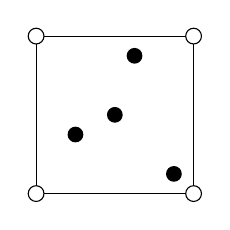
\begin{tikzpicture}
                \draw (0,0) rectangle (2,2);
                \fill[white] (0,0) circle (0.1); \fill[white] (0,2) circle (0.1); \fill[white] (2,0) circle (0.1); \fill[white] (2,2) circle (0.1);
                \draw (0,0) circle (0.1); \draw (0,2) circle (0.1); \draw (2,0) circle (0.1); \draw (2,2) circle (0.1);
                \fill[black] (0.5,0.75) circle (0.1); \fill[black] (1.25,1.75) circle (0.1); \fill[black] (1.75,0.25) circle (0.1); \fill[black] (1,1) circle (0.1);
              \end{tikzpicture}
            \end{column}
            \begin{column}{0.6\textwidth}
              States of particles known at time $t^n$:
              \begin{equation*}
                \left\lbrace\begin{aligned}
                    & \vect{v}^{p,n},\tens{F}^{p,n},\tens{\Pi}^{p,n} \: \rightarrow \:\Ucb^{p,n},\Qcb^{p,n}\\
                    & \vect{X}^{p,n} \: \rightarrow \:M_i^{L,n},K_{ij}^{\alpha,n}
                  \end{aligned}\right.
              \end{equation*}
              
            \end{column}
          \end{columns}
        \end{block}
      \end{column}
    \end{columns}
  \end{footnotesize}
\end{frame}

\begin{frame}{Procedure between $t^n$ and $t^n + \Delta t^n=t^{n+1}$}
  \begin{footnotesize}
    %% Particles -> Nodes
    \begin{equation*}
      \text{Discrete system: }M^L_{i} \frac{\bar{\Ucb}^{i,n+1} - \alert{\bar{\Ucb}^{i,n}}}{\Delta t^n}  - K_{ij}^\alpha \bar{\Fcb}^{j,n}_{\alpha}  + \hat{\Fcb}^{i,n}=  \vect{0}
    \end{equation*}
    \begin{columns}
      \begin{column}{0.4\textwidth}
        \begin{itemize}
        \item[(1)] Computation of matrices $M_i^L$ and $K_{ij}^\alpha$
        \item[(2)] Projection particles $\rightarrow$ nodes
        \end{itemize}
      \end{column}
      \vrule{}
      \begin{column}{0.6\textwidth}
        \begin{block}{Projection particles $\rightarrow$ nodes}
          \begin{columns}
            \begin{column}{0.3\textwidth}
              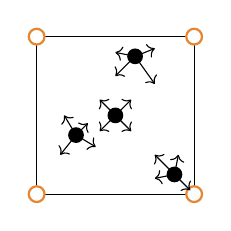
\begin{tikzpicture}
                \draw (0,0) rectangle (2,2);
                \fill[white] (0,0) circle (0.1); \fill[white] (0,2) circle (0.1); \fill[white] (2,0) circle (0.1); \fill[white] (2,2) circle (0.1);
                \draw[Orange,thick] (0,0) circle (0.1); \draw[Orange,thick] (0,2) circle (0.1); \draw[Orange,thick] (2,0) circle (0.1); \draw[Orange,thick] (2,2) circle (0.1);
                \fill[black] (0.5,0.75) circle (0.1); \fill[black] (1.25,1.75) circle (0.1); \fill[black] (1.75,0.25) circle (0.1); \fill[black] (1,1) circle (0.1);
                %% North arrows
                \draw[->,black] (1.25,1.75) -- (1.5,1.85);\draw[->,black] (1.25,1.75) -- (1.,1.8);\draw[->,black] (1.25,1.75) -- (1.,1.5);\draw[->,black] (1.25,1.75) -- (1.5,1.4);
                %% West arrows
                \draw[->,black] (0.5,0.75) -- (0.3,0.5);\draw[->,black] (0.5,0.75) -- (0.35,1.);\draw[->,black] (0.5,0.75) -- (0.75,.6);\draw[->,black] (0.5,0.75) -- (.65,0.9);
                %% Center arrows
                \draw[->,black] (1,1) -- (1.2,1.2);\draw[->,black] (1,1) -- (1.2,0.8);\draw[->,black] (1,1) -- (0.8,1.2);\draw[->,black] (1,1) -- (0.8,0.8);
                %% South arrows
                \draw[->,black] (1.75,0.25) -- (1.95,.05);\draw[->,black] (1.75,0.25) -- (1.8,.5);\draw[->,black] (1.75,0.25) -- (1.5,.5);\draw[->,black] (1.75,0.25) -- (1.5,0.2);
              \end{tikzpicture}
            \end{column}
            \begin{column}{0.6\textwidth}
              \begin{equation*}
                \begin{aligned}
                  & M^{L,n}_i \alert{\bar{\Ucb}^{i,n}} = \sum_{p=1}^{N_p} m_p \bar{\Ucb}^{p,n}\\
                  & M^{L,n}_i \alert{\Qcb^{i,n}} = \sum_{p=1}^{N_p} m_p \Qcb^{p,n}
                \end{aligned}
              \end{equation*}
            \end{column}
          \end{columns}
        \end{block}
      \end{column}
    \end{columns}
  \end{footnotesize}
\end{frame}


\begin{frame}{Procedure between $t^n$ and $t^n + \Delta t^n=t^{n+1}$}
  \begin{footnotesize}
    %% Computation of numerical fluxes (volume + intercell)
    \begin{equation*}
      \text{Discrete system: }M^L_{i} \frac{\bar{\Ucb}^{i,n+1} - \bar{\Ucb}^{i,n}}{\Delta t^n}  - K_{ij}^\alpha \alert{\bar{\Fcb}^{j,n}_{\alpha}}  + \alert{\hat{\Fcb}^{i,n}}=  \vect{0}
    \end{equation*}
    \begin{columns}
      \begin{column}{0.4\textwidth}
        \begin{itemize}
        \item[(1)] Computation of matrices $M_i^L$ and $K_{ij}^\alpha$
        \item[(2)] Projection particles $\rightarrow$ nodes
        \item[(3)] Computation of fluxes
        \end{itemize}
      \end{column}
      \vrule{}
      \begin{column}{0.6\textwidth}
        \begin{block}{Computation of fluxes}
          \begin{columns}
            \begin{column}{0.4\textwidth}
              \begin{block}{\footnotesize Volume fluxes}
                $\bar{\Ucb}^{i,n},\Qcb^{i,n} \rightarrow \bar{\Fcb}^{i,n}_\alpha$
              \end{block}
            \end{column}
            \begin{column}{0.55\textwidth}
              \begin{block}{\footnotesize Intercell fluxes}
                Approximate Riemann solver $\rightarrow \hat{\Fcb}^i$
              \end{block}
            \end{column}
          \end{columns}
        \end{block}
      \end{column}
    \end{columns}
  \end{footnotesize}
\end{frame}

\begin{frame}{Procedure between $t^n$ and $t^n + \Delta t^n=t^{n+1}$}
  \begin{footnotesize}
    %% Time integration 
    \begin{equation*}
      \text{Discrete system: }M^L_{i} \frac{\alert{\bar{\Ucb}^{i,n+1}} - \bar{\Ucb}^{i,n}}{\Delta t^n}  - K_{ij}^\alpha \bar{\Fcb}^{j,n}_{\alpha}  + \hat{\Fcb}^{i,n}=  \vect{0}
    \end{equation*}
    \begin{columns}
      \begin{column}{0.4\textwidth}
        \begin{itemize}
        \item[(1)] Computation of matrices $M_i^L$ and $K_{ij}^\alpha$
        \item[(2)] Projection particles $\rightarrow$ nodes
        \item[(3)] Computation of fluxes
        \item[(4)] Explicit time integration
        \end{itemize}
      \end{column}
      \vrule{}
      \begin{column}{0.6\textwidth}
        \begin{block}{Explicit time integration}
          
          % \begin{columns}
          %   \begin{column}{0.4\textwidth}
              % \begin{tikzpicture}
              %   \draw (0,0) rectangle (2,2);
              %   \fill[white] (0,0) circle (0.1); \fill[white] (0,2) circle (0.1); \fill[white] (2,0) circle (0.1); \fill[white] (2,2) circle (0.1);
              %   \draw (0,0) circle (0.1); \draw (0,2) circle (0.1); \draw (2,0) circle (0.1); \draw (2,2) circle (0.1);
              %   \draw[->,thick] (0,0) -- (0.15,0.15);
              %   \draw[->,thick] (2,0) -- (1.85,0.15);
              %   \draw[->,thick] (2,2) -- (1.85,1.85);
              %   \draw[->,thick] (0,2) -- (.15,1.85);
                
              %   \fill[Orange] (0.5,0.75) circle (0.1); \fill[Orange] (1.25,1.75) circle (0.1); \fill[Orange] (1.75,0.25) circle (0.1); \fill[Orange] (1,1) circle (0.1);
              % \end{tikzpicture}
            % \end{column}
          %   \begin{column}{0.55\textwidth}
          %     \begin{equation*}
          %       \alert{\bar{\Ucb}^{p,n+1}}=\sum_{i=1}^{N_{nodes}} S_{i}(\vect{X}^{p}) \bar{\Ucb}^{i,n+1}
          %     \end{equation*}
          %   \end{column}
          % \end{columns}
        \end{block}
      \end{column}
    \end{columns}
  \end{footnotesize}
\end{frame}

\begin{frame}{Procedure between $t^n$ and $t^n + \Delta t^n=t^{n+1}$}
  \begin{footnotesize}
    %% Interpolation
    \begin{columns}
      \begin{column}{0.4\textwidth}
        \begin{itemize}
        \item[(1)] Computation of matrices $M_i^L$ and $K_{ij}^\alpha$
        \item[(2)] Projection particles $\rightarrow$ nodes
        \item[(3)] Computation of fluxes
        \item[(4)] Explicit time integration
        \item[(5)] Projection nodes $\rightarrow$ particles 
        \end{itemize}
      \end{column}
      \vrule{}
      \begin{column}{0.6\textwidth}
        \begin{block}{Projection nodes $\rightarrow$ particles}
          
          \begin{columns}
            \begin{column}{0.4\textwidth}
              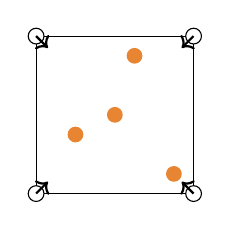
\begin{tikzpicture}
                \draw (0,0) rectangle (2,2);
                \fill[white] (0,0) circle (0.1); \fill[white] (0,2) circle (0.1); \fill[white] (2,0) circle (0.1); \fill[white] (2,2) circle (0.1);
                \draw (0,0) circle (0.1); \draw (0,2) circle (0.1); \draw (2,0) circle (0.1); \draw (2,2) circle (0.1);
                \draw[->,thick] (0,0) -- (0.15,0.15);
                \draw[->,thick] (2,0) -- (1.85,0.15);
                \draw[->,thick] (2,2) -- (1.85,1.85);
                \draw[->,thick] (0,2) -- (.15,1.85);
                
                \fill[Orange] (0.5,0.75) circle (0.1); \fill[Orange] (1.25,1.75) circle (0.1); \fill[Orange] (1.75,0.25) circle (0.1); \fill[Orange] (1,1) circle (0.1);
              \end{tikzpicture}
            \end{column}
            \begin{column}{0.55\textwidth}
              \begin{equation*}
                \alert{\bar{\Ucb}^{p,n+1}}=\sum_{i=1}^{N_{nodes}} S_{i}(\vect{X}^{p}) \bar{\Ucb}^{i,n+1}
              \end{equation*}
            \end{column}
          \end{columns}
        \end{block}
      \end{column}
    \end{columns}
  \end{footnotesize}
\end{frame}

\begin{frame}{Procedure between $t^n$ and $t^n + \Delta t^n=t^{n+1}$}
  \begin{footnotesize}
    %% Kinematic and constitutive updates
    \begin{columns}
      \begin{column}{0.4\textwidth}
        \begin{itemize}
        \item[(1)] Computation of matrices $M_i^L$ and $K_{ij}^\alpha$
        \item[(2)] Projection particles $\rightarrow$ nodes
        \item[(3)] Computation of fluxes
        \item[(4)] Explicit time integration
        \item[(5)] Projection nodes $\rightarrow$ particles 
        \item[(6)] Kinematics and constitutive updates
        \end{itemize}
      \end{column}
      \vrule{}
      \begin{column}{0.6\textwidth}
        \begin{block}{Kinematics and constitutive updates}
          \begin{columns}
            \begin{column}{0.4\textwidth}
              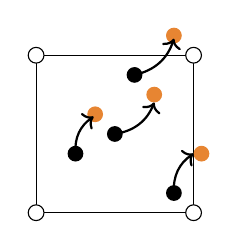
\begin{tikzpicture}
                \draw (0,0) rectangle (2,2);
                \fill[white] (0,0) circle (0.1); \fill[white] (0,2) circle (0.1); \fill[white] (2,0) circle (0.1); \fill[white] (2,2) circle (0.1);
                \draw (0,0) circle (0.1); \draw (0,2) circle (0.1); \draw (2,0) circle (0.1); \draw (2,2) circle (0.1);
                \fill[black] (0.5,0.75) circle (0.1); \fill[black] (1.25,1.75) circle (0.1); \fill[black] (1.75,0.25) circle (0.1); \fill[black] (1,1) circle (0.1);
                \fill[Orange] (0.75,1.25) circle (0.1); \fill[Orange] (1.75,2.25) circle (0.1); \fill[Orange] (2.1,0.75) circle (0.1); \fill[Orange] (1.5,1.5) circle (0.1);
                \path[->,thick,black] (0.5,0.75) edge[bend left] (0.73,1.22);
                \path[->,thick,black] (1.25,1.75) edge[bend right] (1.75,2.21);
                \path[->,thick,black](1.75,0.25) edge[bend left] (2.,0.75);
                \path[->,thick,black](1,1) edge[bend right] (1.5,1.4);
              \end{tikzpicture}
            \end{column}
            \begin{column}{0.55\textwidth}
              \begin{flalign*}
                \begin{aligned}
                  & \alert{\tens{\Pi}^{p,n+1}}=g(\tens{F}^{p,n+1})\\
                  & \alert{\vect{\varphi}^{p,n+1}}= \vect{\varphi}^{p,n} +\Delta t^n \vect{v}^{p,n+1}
                \end{aligned}
              \end{flalign*}
            \end{column}
          \end{columns}
        \end{block}
      \end{column}
    \end{columns}
  \end{footnotesize}
\end{frame}
      
\begin{frame}{Procedure between $t^n$ and $t^n + \Delta t^n=t^{n+1}$}
  \begin{footnotesize}
    %% Rebuild the grid if needed
    \begin{columns}
      \begin{column}{0.4\textwidth}
        \begin{itemize}
        \item[(1)] Computation of matrices $M_i^L$ and $K_{ij}^\alpha$
        \item[(2)] Projection particles $\rightarrow$ nodes
        \item[(3)] Computation of fluxes
        \item[(4)] Explicit time integration
        \item[(5)] Projection nodes $\rightarrow$ particles 
        \item[(6)] Kinematics and constitutive updates
        \item[(7)] Reconstruction of the grid (if needed) 
        \end{itemize}
      \end{column}
      \vrule{}
      \begin{column}{0.6\textwidth}
        \begin{block}{Reconstruction of the grid (if needed)}
          \begin{columns}
            \begin{column}{0.4\textwidth}
              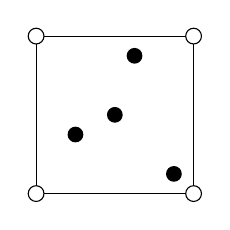
\begin{tikzpicture}
                \draw (0,0) rectangle (2,2);
                \fill[white] (0,0) circle (0.1); \fill[white] (0,2) circle (0.1); \fill[white] (2,0) circle (0.1); \fill[white] (2,2) circle (0.1);
                \draw (0,0) circle (0.1); \draw (0,2) circle (0.1); \draw (2,0) circle (0.1); \draw (2,2) circle (0.1);
                \fill[black] (0.5,0.75) circle (0.1); \fill[black] (1.25,1.75) circle (0.1); \fill[black] (1.75,0.25) circle (0.1); \fill[black] (1,1) circle (0.1);
              \end{tikzpicture}
            \end{column}
            \begin{column}{0.55\textwidth}
              \centering
              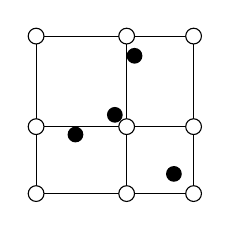
\begin{tikzpicture}
                \draw (0,0) rectangle (2.,2.);
                \draw (1.15,0.85) rectangle (2.,0);
                \draw (1.15,0.85) rectangle (2.,2);
                \draw (1.15,0.85) rectangle (0.,2);
                %% Old nodes
                \fill[white] (0,0) circle (0.1);
                \fill[white] (0,2) circle (0.1);
                \fill[white] (2,0) circle (0.1);
                \fill[white] (2,2) circle (0.1);
                \draw (0,0) circle (0.1);
                \draw (0,2) circle (0.1);
                \draw (2,0) circle (0.1);
                \draw (2,2) circle (0.1);
                
                %% Added nodes
                \fill[white] (1.15,0.85) circle (0.1);
                \fill[white] (0,0.85) circle (0.1);
                \fill[white] (2,0.85) circle (0.1);
                \fill[white] (1.15,0) circle (0.1);
                \fill[white] (1.15,2) circle (0.1);
                \draw (1.15,0.85) circle (0.1);
                \draw (0,0.85) circle (0.1);
                \draw (2,0.85) circle (0.1);
                \draw (1.15,0) circle (0.1);
                \draw (1.15,2) circle (0.1);
                
                %% Particles
                \fill[black] (0.5,0.75) circle (0.1); \fill[black] (1.25,1.75) circle (0.1); \fill[black] (1.75,0.25) circle (0.1); \fill[black] (1,1) circle (0.1);
              \end{tikzpicture}
            \end{column}
          \end{columns}
        \end{block}
      \end{column}
    \end{columns}
  \end{footnotesize}
\end{frame}
%%% Local Variables:
%%% mode: latex
%%% TeX-master: "../presentation"
%%% End:



\subsection{Stability analysis}
\begin{frame}{Linear advection equation of an arbitrary quantity $q$}%{One-dimensional problems}
  \begin{block}{Scheme equation (finite difference sense)}
    \begin{footnotesize}
      \begin{equation*}
        \bar{q}^{p,n+1}=\sum_{k=1}^{N_p}H_{pk}(\vect{X}^p,\vect{X}^k,\text{CFL})\bar{q}^{k,n}
      \end{equation*}
    \end{footnotesize}
  \end{block}
  \begin{block}{von-Neumann linear stability analysis}
    \begin{footnotesize}
      The numerical scheme is stable if:
      \begin{equation*}
        \sum_{k=1}^{N_p}\abs{H_{pk}} \leq 1 \quad \forall p
      \end{equation*}
      \alert{$\Rightarrow$ find the maximal CFL number ensuring the stability}
    \end{footnotesize}
  \end{block}\pause
  \metroset{block=fill}
  \begin{footnotesize}
    \begin{block}{Particular case: one particle per cell}
      The \textbf{first-order} FVM is recovered $\rightarrow$ CFL improved compared to MPM and DGFEM
    \end{block}
  \end{footnotesize}
\end{frame}


%%% Local Variables:
%%% mode: latex
%%% TeX-master: "../presentation"
%%% End:




\section{Numerical simulations}

\subsection{Linearized geometrical framework}
\begin{frame}{\href{section4/animation/elasticity_stress/video.mp4}{Plane strain elasticity}}
  \begin{overprint}
    \onslide<1>
    \vspace{-1.cm}
    \begin{columns}
      \begin{column}{0.42\linewidth}
        \input{section4/pgfFigures/2d_square}
      \end{column}

      \begin{column}{0.6\linewidth}
        \vspace{1.5cm}
        \centering
        \phantom{\begin{tikzpicture}
  \begin{groupplot}[group style={group size=2 by 1,
ylabels at=edge left, yticklabels at=edge left,horizontal sep=1.5ex,
xticklabels at=edge bottom,xlabels at=edge bottom},
ymajorgrids=true,xmajorgrids=true,xlabel=$x \: (m)$,
axis on top,scale only axis,width=0.43\linewidth, every x tick scale label/.style={at={(xticklabel* cs:1.05,0.75cm)},anchor=near yticklabel},ymin=-0.5e6,ymax=.5e9,xmin=0,xmax=3]
\nextgroupplot[ylabel=$\sigma_{11}\: (Pa)$,title={$t=2.5 \times 10^{-4} \: s$},every y tick scale label/.style={at={(-0.,1.1)}}]
\addplot[Red,very thick,no markers] table[x=Points:0,y=S11] {section4/csvFiles/2delast_fem_115.csv};

\addplot[Blue,very thick,mark=+,only marks,mark size=3pt] table[x=Points:0,y=stress_11] {section4/csvFiles/2delast_ctu1ppc_115.csv};
\addplot[Purple,very thick,mark=asterisk,only marks,mark size=2pt] table[x=Points:0,y=stress_11] {section4/csvFiles/2delast_ctu4ppc_115.csv};
\addplot[Orange,very thick,mark=x,only marks,mark size=3pt] table[x=Points:0,y=mpm_S11] {section4/csvFiles/2delast_mpm_115.csv};

\nextgroupplot[legend style={at={($(0.22,-0.3)+(1.cm,0cm)$)},legend columns=2},xlabel=$x (m)$,title={$t=1.0 \times 10^{-3} \: s$},ytick scale label code/.code={}]
\addplot[Red,very thick,no markers] table[x=Points:0,y=S11] {section4/csvFiles/2delast_fem_338.csv};
\addplot[Blue,very thick,mark=+,only marks,mark size=3pt] table[x=Points:0,y=stress_11] {section4/csvFiles/2delast_ctu1ppc_338.csv};
\addplot[Purple,very thick,mark=asterisk,only marks,mark size=2pt] table[x=Points:0,y=stress_11] {section4/csvFiles/2delast_ctu4ppc_338.csv};
\addplot[Orange,very thick,mark=x,only marks,mark size=3pt] table[x=Points:0,y=mpm_S11] {section4/csvFiles/2delast_mpm_338.csv};
\addlegendentry{fem}
\addlegendentry{ctu 1ppc}
\addlegendentry{ctu 4ppc}
\addlegendentry{mpm}
   
  \end{groupplot}
\end{tikzpicture}


%%% Local Variables:
%%% mode: latex
%%% TeX-master: "../../aRenaud"
%%% End:




































%%% Local Variables:
%%% mode: latex
%%% TeX-master: "../../mainManuscript"
%%% End:
}
      \end{column}
      
    \end{columns}
    \onslide<2>
    \vspace{-1.cm}
    \begin{columns}
      \begin{column}{0.42\linewidth}
        \movie[height=.7\paperheight,width=1.\linewidth,showcontrols,loop,poster,autostart]{%\input{section4/pgfFigures/2d_square}
        }{section4/animation/elasticity_stress/video.mp4}
      \end{column}

      \begin{column}{0.6\linewidth}
        \vspace{1.5cm}
        \centering
        \begin{tikzpicture}
  \begin{groupplot}[group style={group size=2 by 1,
ylabels at=edge left, yticklabels at=edge left,horizontal sep=1.5ex,
xticklabels at=edge bottom,xlabels at=edge bottom},
ymajorgrids=true,xmajorgrids=true,xlabel=$x \: (m)$,
axis on top,scale only axis,width=0.43\linewidth, every x tick scale label/.style={at={(xticklabel* cs:1.05,0.75cm)},anchor=near yticklabel},ymin=-0.5e6,ymax=.5e9,xmin=0,xmax=3]
\nextgroupplot[ylabel=$\sigma_{11}\: (Pa)$,title={$t=2.5 \times 10^{-4} \: s$},every y tick scale label/.style={at={(-0.,1.1)}}]
\addplot[Red,very thick,no markers] table[x=Points:0,y=S11] {section4/csvFiles/2delast_fem_115.csv};

\addplot[Blue,very thick,mark=+,only marks,mark size=3pt] table[x=Points:0,y=stress_11] {section4/csvFiles/2delast_ctu1ppc_115.csv};
\addplot[Purple,very thick,mark=asterisk,only marks,mark size=2pt] table[x=Points:0,y=stress_11] {section4/csvFiles/2delast_ctu4ppc_115.csv};
\addplot[Orange,very thick,mark=x,only marks,mark size=3pt] table[x=Points:0,y=mpm_S11] {section4/csvFiles/2delast_mpm_115.csv};

\nextgroupplot[legend style={at={($(0.22,-0.3)+(1.cm,0cm)$)},legend columns=2},xlabel=$x (m)$,title={$t=1.0 \times 10^{-3} \: s$},ytick scale label code/.code={}]
\addplot[Red,very thick,no markers] table[x=Points:0,y=S11] {section4/csvFiles/2delast_fem_338.csv};
\addplot[Blue,very thick,mark=+,only marks,mark size=3pt] table[x=Points:0,y=stress_11] {section4/csvFiles/2delast_ctu1ppc_338.csv};
\addplot[Purple,very thick,mark=asterisk,only marks,mark size=2pt] table[x=Points:0,y=stress_11] {section4/csvFiles/2delast_ctu4ppc_338.csv};
\addplot[Orange,very thick,mark=x,only marks,mark size=3pt] table[x=Points:0,y=mpm_S11] {section4/csvFiles/2delast_mpm_338.csv};
\addlegendentry{fem}
\addlegendentry{ctu 1ppc}
\addlegendentry{ctu 4ppc}
\addlegendentry{mpm}
   
  \end{groupplot}
\end{tikzpicture}


%%% Local Variables:
%%% mode: latex
%%% TeX-master: "../../aRenaud"
%%% End:




































%%% Local Variables:
%%% mode: latex
%%% TeX-master: "../../mainManuscript"
%%% End:

      \end{column}
    \end{columns}
  \end{overprint}
\end{frame}


\begin{frame}{Plane strain elastoplasticity}
  \begin{overprint}
    \onslide<1>
    \vspace{0.25cm}
    \centering
    \movie[height=.7\paperheight,width=.75\linewidth,showcontrols,loop,poster,autostart]{
    }{section4/animation/elastoplasticity/video.ogv}
    \onslide<2>
    \centering
    \begin{tikzpicture}[scale=0.49]
  \begin{groupplot}[group style={group size=1 by 2,
ylabels at=edge left, yticklabels at=edge left,horizontal sep=3.ex,vertical sep=4.ex,
xticklabels at=edge bottom,xlabels at=edge bottom},
ymajorgrids=true,xmajorgrids=true,
axis on top,scale only axis, every x tick scale label/.style={at={(xticklabel* cs:1.05,0.75cm)},anchor=near yticklabel}]
\nextgroupplot[ylabel=\normalsize $\sigma_{11}$ (Pa)]
\addplot[Red,very thick,no markers] table[x=Points:0,y=S11] {appendix/csvFiles/2dEP_fem_115.csv};
\addplot[Blue,very thick,mark=+,only marks,mark size=3pt] table[x=Points:0,y=stress_11] {appendix/csvFiles/2dEP_ctu1ppc_115.csv};
\addplot[Purple,very thick,mark=square,only marks] table[x=Points:0,y=stress_11] {appendix/csvFiles/2dEP_ctu4ppc_115.csv};
\addplot[Orange,very thick,mark=x,only marks,mark size=3pt] table[x=Points:0,y= mpm_S11] {appendix/csvFiles/2dEP_mpm_115.csv};

% \nextgroupplot[title={(b) $t=1.0 \times 10^{-3} \: s$},ymin=-0.5e6,ymax=1.5e9]
% \addplot[Red,very thick,no markers] table[x=Points:0,y=S11] {appendix/csvFiles/2dEP_fem_338.csv};
% \addplot[Blue,very thick,mark=+,only marks,mark size=3pt] table[x=Points:0,y=stress_11] {appendix/csvFiles/2dEP_ctu1ppc_338.csv};
% \addplot[Purple,very thick,mark=square,only marks] table[x=Points:0,y=stress_11] {appendix/csvFiles/2dEP_ctu4ppc_338.csv};
% \addplot[Orange,very thick,mark=x,only marks,mark size=3pt] table[x=Points:0,y= mpm_S11] {appendix/csvFiles/2dEP_mpm_338.csv};

\nextgroupplot[%legend style={at={($(0.12,-0.35)+(5cm,5cm)$)},legend columns=1}
legend pos={north east},
,ylabel=\normalsize $\eps^p_{11}$,xlabel=\normalsize $x$ (m)]
\addplot[Red,very thick,no markers] table[x=Points:0,y=EP11] {appendix/csvFiles/2dEP_fem_115.csv};
\addplot[Blue,very thick,mark=+,only marks,mark size=3pt] table[x=Points:0,y=epsp_11] {appendix/csvFiles/2dEP_ctu1ppc_115.csv};
\addplot[Purple,very thick,mark=square,only marks] table[x=Points:0,y=epsp_11] {appendix/csvFiles/2dEP_ctu4ppc_115.csv};
\addplot[Orange,very thick,mark=x,only marks,mark size=3pt] table[x=Points:0,y= mpm_epsp11] {appendix/csvFiles/2dEP_mpm_115.csv};

% \nextgroupplot[legend style={at={($(0.12,-0.35)+(0.9cm,1cm)$)},legend columns=2},xlabel=$x (m)$,ymin=-0.1e-3,ymax=6.75e-3]
% \addplot[Red,very thick,no markers] table[x=Points:0,y=EP11] {appendix/csvFiles/2dEP_fem_338.csv};
% \addplot[Blue,very thick,mark=+,only marks,mark size=3pt] table[x=Points:0,y=epsp_11] {appendix/csvFiles/2dEP_ctu1ppc_338.csv};
% \addplot[Purple,very thick,mark=square,only marks] table[x=Points:0,y=epsp_11] {appendix/csvFiles/2dEP_ctu4ppc_338.csv};
% \addplot[Orange,very thick,mark=x,only marks,mark size=3pt] table[x=Points:0,y= mpm_epsp11] {appendix/csvFiles/2dEP_mpm_338.csv};
\addlegendentry{fem}
\addlegendentry{ctu 1ppc}
\addlegendentry{ctu 4ppc}
\addlegendentry{mpm}
   
  \end{groupplot}
\end{tikzpicture}


%%% Local Variables:
%%% mode: latex
%%% TeX-master: "../../presentation"
%%% End:




































%%% Local Variables:
%%% mode: latex
%%% TeX-master: "../../presentation"
%%% End:

  \end{overprint}

\end{frame}
%%% Local Variables:
%%% mode: latex
%%% TeX-master: "../aRenaud"
%%% End:
\subsection{Large strains framework}
% \begin{frame}
% \begin{tikzpicture}[remember picture,overlay]
%   \node[anchor=south west, inner sep=0pt] at (current page.south west) {%
%     \includemedia[
%     addresource=section4/animation/hyperelasticity_velo/video.mp4,
%     activate=pageopen,transparent,
%     flashvars={source=section4/animation/hyperelasticity_velo/video.mp4},
%     width=\paperwidth,height=\paperheight
%     ]{}{VPlayer.swf}%
%   };
% \end{tikzpicture}
% \end{frame}

\begin{frame}%{\href{section4/animation/hyperelasticity_velo/video.mp4}{2D hyperelasticity}}
  \begin{center}
    % \movie[width=1.\linewidth,showcontrols,loop]{\input{section4/pgfFigures/2d_square}}{section4/animation/hyperelasticity_velo/video.mp4}
    \href{section4/animation/hyperelasticity_velo/video.mp4}{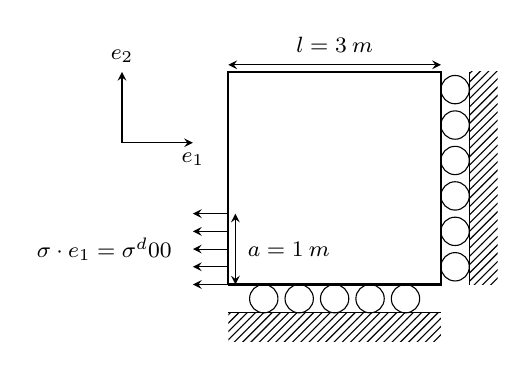
\begin{tikzpicture}[scale=0.9]
  \draw[thick] (0,0) --(3,0)--(3,3)--(0,3)--(0,0);
  \foreach \x in {0.5,1.,...,2.5} 
  \draw(\x,-0.2)circle(0.2);
  \foreach \x in {0.25,0.75,...,2.75} 
  \draw(3.2,\x)circle(0.2);
  \draw(0,-0.4)--(3.,-0.4);
  \draw(3.4,0)--(3.4,3);
  \fill [pattern=north east lines](0.0,-0.8)rectangle+(3,0.4);
  \fill [pattern=north east lines](3.4,0.)rectangle+(0.4,3);
  \draw[>=stealth,<->](0,3.1)--node[above=1pt]{\footnotesize $l=3 \: m$}(3,3.1);
  \draw[>=stealth,<->](0.1,0)--node[right=1pt]{\footnotesize $a=1 \: m$}(0.1,1);
  \foreach \x in {0.,0.25,...,1} 
  \draw[>=stealth,<-] (-0.5,\x)--(0.,\x);
  \node(a)at(-1.75,0.5){\footnotesize $\tens{\sigma}\cdot\vect{e}_1=\matrice{\sigma^d\\0 \\0}$}; 
  \draw[>=stealth,->](-1.5,2)--(-0.5,2)node(a)[anchor=north]{\footnotesize $\vect{e}_1$};
  \draw[>=stealth,->](-1.5,2)--(-1.5,3)node(a)[anchor=south]{\footnotesize $\vect{e}_2$};
\end{tikzpicture}
% \input{section4/pgfFigures/2d_square}
}
    % \movie[height = \paperheight, width = \paperwidth, poster,showcontrols,loop]{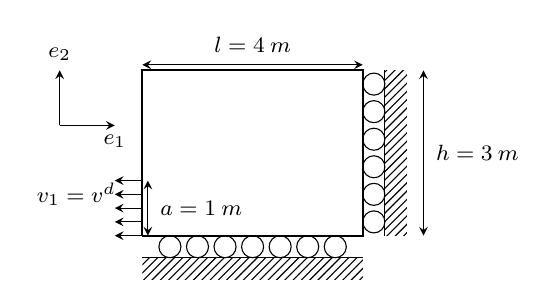
\begin{tikzpicture}[scale=0.7]
  \draw[thick] (0,0) --(4,0)--(4,3)--(0,3)--(0,0);
  \foreach \x in {0.5,1.,...,3.5} 
  \draw(\x,-0.2)circle(0.2);
  \foreach \x in {0.25,0.75,...,2.75} 
  \draw(4.2,\x)circle(0.2);
  \draw(0,-0.4)--(4.,-0.4);
  \draw(4.4,0)--(4.4,3);
  \fill [pattern=north east lines](0.0,-0.8)rectangle+(4,0.4);
  \fill [pattern=north east lines](4.4,0.)rectangle+(0.4,3);
  \draw[>=stealth,<->](5.1,0)--node[right=1pt]{\footnotesize $h=3 \: m$}(5.1,3);
  \draw[>=stealth,<->](0,3.1)--node[above=1pt]{\footnotesize $l=4 \: m$}(4,3.1);
  \draw[>=stealth,<->](0.1,0)--node[right=1pt]{\footnotesize $a=1 \: m$}(0.1,1);
  \foreach \x in {0.,0.25,...,1} 
  \draw[>=stealth,<-] (-0.5,\x)--(0.,\x);
  \node(a)at(-1.2,0.75){\footnotesize $v_1=v^d$}; 
  \draw[>=stealth,->](-1.5,2)--(-0.5,2)node(a)[anchor=north]{\footnotesize $\vect{e}_1$};
  \draw[>=stealth,->](-1.5,2)--(-1.5,3)node(a)[anchor=south]{\footnotesize $\vect{e}_2$};
\end{tikzpicture}

%%% Local Variables:
%%% mode: latex
%%% TeX-master: "../../mainManuscript"
%%% End:}{section4/animation/hyperelasticity_velo/video.mp4}
    % \animategraphics[loop,controls,width=1.\linewidth,autoplay]{10}{animation/hyperelasticity_velo/animation-}{0}{3}
  \end{center}
\end{frame}


%%% Local Variables:
%%% mode: latex
%%% TeX-master: "../aRenaud"
%%% End:




%%% Local Variables:
%%% mode: latex
%%% TeX-master: "../aRenaud"
%%% End:


\section*{Conclusion}
\begin{withoutheadline}
  \begin{frame}[standout]{\text{Conclusion of part I}}
    \setbeamercolor{alerted text}{fg=white}
    \setbeamercolor{normal text}{ fg= white , bg= CNBlue }
    \begin{footnotesize}
      \begin{block}{\text{Development of the DGMPM in total Lagrangian}}
        \begin{columns}
          \begin{column}{0.4\textwidth}
            \begin{block}{Ingredients}
              \begin{itemize}
              \item Riemann solver
              \item Arbitrary grid
              \item DG approximation
              \item Classical constitutive integrators
              \end{itemize}
            \end{block}
          \end{column}
          \begin{column}{0.5\textwidth}
            \begin{block}{Possibilities}
              \begin{itemize}
              \item Take into acount the characteristic structure
              \item Adapt the grid without additional projection
              \item Locally high-order approximation
              \item Control of time-stepping
              \end{itemize}
            \end{block}
          \end{column}
        \end{columns}
      \end{block}
    \end{footnotesize}
  \end{frame}
\end{withoutheadline}
\part{2D Elastoplastic hyperbolic problems}
\label{part:part2}
\begin{withoutheadline}
\begin{frame}{Multi-dimensional elastic-plastic solids}
  
  \begin{block}{Continuum point of view}
    Important for solid mechanics applications (residual states)\\
    \centering
    \movie[height = 0.25\paperheight,width=0.2\linewidth,loop,poster]{}{section1/animation/output3.mp4}
  \end{block}
  
  \begin{block}{Numerical methods}
    Improvement enabled by the characteristic structure considered 
  \end{block}
  \pause
  \metroset{block=fill}
  \begin{block}{Objective 2}
    Identify the response of two-dimensional elastic-plastic solids to dynamic loadings
    \begin{itemize}
    \item Better understanding of the features of solutions in the elastic-plastic regime
    \item Building of dedicated approximate Riemann solvers
    \end{itemize}
  \end{block} 
  % \end{block}
\end{frame}
\end{withoutheadline}

\section{General framework}
%% Biblio section

\subsection{Historical review}
%% Problèmes traités -- approche expérimentale pour la confirmation
%% Type de solutions
%% Simple waves even for linear hardening in contrast to one-dimensional problems

\begin{frame}{Thin-walled tube problem}%{Historical review}
  %% References: Lin_et_Ballman,Li_planeStress_EP,Wu_experimental,Ting73,Clifton_exp2,Valanis,Clifton_exp,Ting69,Bleich,Clifton,CRISTESCU19591605,Rakhmatulin
  \begin{overprint}
    \onslide<1>
    \begin{columns}
      \begin{column}{0.4\textwidth}
        \begin{block}{\footnotesize Semi-infinite medium}
          % \centering
          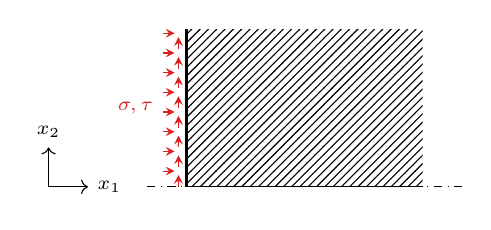
\begin{tikzpicture}
            \begin{scope}[shift={(-1.75,0)}]
              \draw[->] (0,0) -- (0.5,0) node[right] {\scriptsize $x_1$};
              \draw[->] (0,0) -- (0,0.5) node[above] {\scriptsize $x_2$};
            \end{scope}
            \draw (0,0) -- (3,.0);
            \draw[very thick] (0,0) -- (0,2.);
            \fill [pattern=north east lines] (0,0) rectangle (3.,2.);
            \draw[dash dot] (-0.5,0) -- (3.5,0);% node[right] {\footnotesize $x_1$};
            % \draw[->,dash dot] (0,0) -- (0,2.5) node[above] {\footnotesize $x_2$};
            \foreach \y in {0,0.25,...,1.75}
            \draw[Red,->,>=stealth] (-0.1,\y) -- (-0.1,\y+0.15);
            \foreach \y in {0,0.25,...,1.75}
            \draw[Red,->,>=stealth] (-0.30,\y+0.20) -- (-0.15,\y+0.20);
            \node[Red,left] at (-0.3,1.) {\scriptsize $\sigma,\tau$};
          \end{tikzpicture}  
        \end{block}
      \end{column}
      \begin{column}{0.62\textwidth}
        \begin{footnotesize}
          \begin{block}{\footnotesize Elastic solution}
            \begin{columns}
              \begin{column}{0.35\textwidth}
                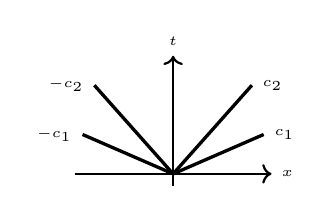
\begin{tikzpicture}[scale=0.5]
                  \draw[thick,->] (-2.5,0) -- (2.5,0) node[right] {\tiny $x$};
                  \draw[thick,->] (-0.,-0.3) -- (0,3) node[above] {\tiny $t$};
                  \draw[very thick] (0,0) -- (2.3,1.) node[right] {\tiny $c_1$};
                  \draw[very thick] (0,0) -- (-2.3,1.) node[left] {\tiny $-c_1$};
                  \draw[very thick] (0,0) -- (2.,2.25) node[right] {\tiny $c_2$};
                  \draw[very thick] (0,0) -- (-2.,2.25) node[left] {\tiny $-c_2$};
                \end{tikzpicture}
              \end{column}
              \begin{column}{0.6\textwidth}
                \begin{itemize}
                \item[] pressure and shear waves: $c_1,c_2$
                \item[] discontinuous waves
                \end{itemize}
              \end{column}
            \end{columns}
          \end{block}
        \end{footnotesize}
      \end{column}
    \end{columns}
    \onslide<2>
    \begin{columns}
      \begin{column}{0.4\textwidth}
        \begin{block}{\footnotesize Semi-infinite medium}
          % \centering
          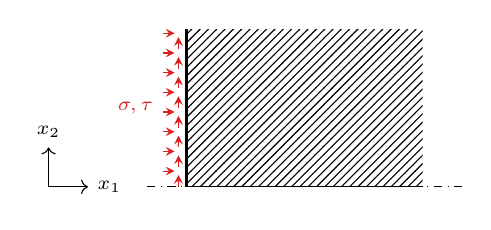
\begin{tikzpicture}
            \begin{scope}[shift={(-1.75,0)}]
              \draw[->] (0,0) -- (0.5,0) node[right] {\scriptsize $x_1$};
              \draw[->] (0,0) -- (0,0.5) node[above] {\scriptsize $x_2$};
            \end{scope}
            \draw (0,0) -- (3,.0);
            \draw[very thick] (0,0) -- (0,2.);
            \fill [pattern=north east lines] (0,0) rectangle (3.,2.);
            \draw[dash dot] (-0.5,0) -- (3.5,0);% node[right] {\footnotesize $x_1$};
            % \draw[->,dash dot] (0,0) -- (0,2.5) node[above] {\footnotesize $x_2$};
            \foreach \y in {0,0.25,...,1.75}
            \draw[Red,->,>=stealth] (-0.1,\y) -- (-0.1,\y+0.15);
            \foreach \y in {0,0.25,...,1.75}
            \draw[Red,->,>=stealth] (-0.30,\y+0.20) -- (-0.15,\y+0.20);
            \node[Red,left] at (-0.3,1.) {\scriptsize $\sigma,\tau$};
          \end{tikzpicture}  
        \end{block}
      \end{column}
      \begin{column}{0.62\textwidth}
        \begin{footnotesize}
          \begin{block}{\footnotesize Elastic-\alert{plastic} solution \cite{CRISTESCU19591605,Rakhmatulin}}
            \begin{columns}
              \begin{column}{0.35\textwidth}
                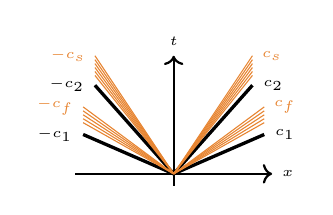
\begin{tikzpicture}[scale=0.5]
                  \draw[thick,->] (-2.5,0) -- (2.5,0) node[right] {\tiny $x$};
                  \draw[thick,->] (-0.,-0.3) -- (0,3) node[above] {\tiny $t$};
                  \draw[very thick] (0,0) -- (2.3,1.) node[right] {\tiny $c_1$};
                  \draw[very thick] (0,0) -- (-2.3,1.) node[left] {\tiny $-c_1$};
                  \draw[very thick] (0,0) -- (2.,2.25) node[right] {\tiny $c_2$};
                  \draw[very thick] (0,0) -- (-2.,2.25) node[left] {\tiny $-c_2$};
                  \foreach \x in {1.3,1.4,1.5,1.6,1.7}
                  {\draw[Orange] (0,0)-- (2.3,\x);
                    \draw[Orange] (0,0)-- (-2.3,\x);}
                  \node[Orange,right] at (2.3,1.7) {\tiny $c_f$};
                  \node[Orange,left] at (-2.3,1.7) {\tiny $-c_f$};
                  \foreach \x in {2.5,2.6,2.7,2.8,2.9,3.}
                  {\draw[Orange] (0,0)-- (2,\x);
                    \draw[Orange] (0,0)-- (-2,\x);}
                  \node[Orange,right] at (2,3) {\tiny $c_s$};
                  \node[Orange,left] at (-2,3) {\tiny $-c_s$};
                \end{tikzpicture}
              \end{column}
              \begin{column}{0.6\textwidth}
                \begin{itemize}
                \item[] fast and slow simple waves: $c_f,c_s$
                \item[] combined-stress waves
                \end{itemize}
              \end{column}
            \end{columns}
          \end{block}
        \end{footnotesize}
      \end{column}
    \end{columns}
    \footnoteCite{CRISTESCU19591605,Rakhmatulin}
  \end{overprint}
\end{frame}


\begin{frame}{Thin-walled tube problem}
  %% Détailler travaux de clifton, comment il en arrive à des trajets élémentaires
  %% Problème de Picard
  \begin{block}{Characteristic analysis of the elastic-plastic hyperbolic system \cite{Clifton}}
    \begin{footnotesize}
      \begin{columns}
        \begin{column}{0.6\textwidth}
          \begin{itemize}
            % \item ODEs governing the evolution of stress and velocity through both simple waves
          \item[] ODEs through simple waves: $d\tau=\psi(\tens{\sigma})d\sigma$ 
            \begin{itemize}
            \item \footnotesize integration $\rightarrow$ loading paths
            \item \footnotesize mathematical study $\rightarrow$ solution of Picard's problem
            \end{itemize}
            \centering
            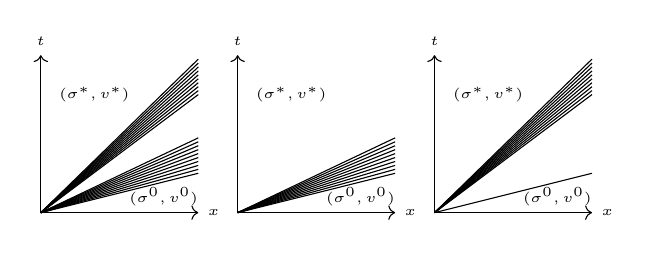
\begin{tikzpicture}
              \draw[->] (0,0) -- (2,0) node[right] {\tiny $x$};
              \draw[->] (0,0) -- (0,2) node[above] {\tiny $t$};
              \node[right] at (1,0.2) {\tiny $(\tens{\sigma}^0,\vect{v}^0)$};
              \draw (0,0) -- (2,0.5);
              \foreach \y in {0.55,0.6,...,1.}
              \draw (0,0) -- (2,\y);
              \foreach \y in {1.5,1.55,...,2.}
              \draw (0,0) -- (2,\y);
              \node[left] at (1.25,1.5) {\tiny $(\tens{\sigma}^*,\vect{v}^*)$};
              \begin{scope}[shift={(2.5,0)}]
                \draw[->] (0,0) -- (2,0) node[right] {\tiny $x$};
                \draw[->] (0,0) -- (0,2) node[above] {\tiny $t$};
                \node[right] at (1,0.2) {\tiny $(\tens{\sigma}^0,\vect{v}^0)$};
                \draw (0,0) -- (2,0.5);
                \foreach \y in {0.55,0.6,...,1.}
                \draw (0,0) -- (2,\y);
                % \foreach \y in {1.5,1.55,...,2.}
                % \draw (0,0) -- (2,\y);
                \node[left] at (1.25,1.5) {\tiny $(\tens{\sigma}^*,\vect{v}^*)$};
              \end{scope}
              \begin{scope}[shift={(5,0)}]
                \draw[->] (0,0) -- (2,0) node[right] {\tiny $x$};
                \draw[->] (0,0) -- (0,2) node[above] {\tiny $t$};
                \node[right] at (1,0.2) {\tiny $(\tens{\sigma}^0,\vect{v}^0)$};
                \draw (0,0) -- (2,0.5);
                \foreach \y in {1.5,1.55,...,2.}
                \draw (0,0) -- (2,\y);
                \node[left] at (1.25,1.5) {\tiny $(\tens{\sigma}^*,\vect{v}^*)$};
              \end{scope}
            \end{tikzpicture}
          %\item confirmed by experimental data \cite{Clifton_exp}
          \end{itemize}
        \end{column}
        \begin{column}{0.43\textwidth}
          \vskip 5pt
          \centering
          \begin{tikzpicture}[scale=0.9]
  \begin{axis}[ymajorgrids=true,xmajorgrids=true,ylabel=$\sigma_{12}$,xlabel=$\sigma_{11}$,xmax=2.e8]
    %%
    \addplot[Green,mark=x,only marks,mark repeat=15,very thick] table [x=sigma_11,y=sigma_12] {chapter5/pgfFigures/pgf_thinWalledTubeSlowWave/slowStressPlane_Stress0.pgf};
    \addplot[Green,thick] table [x=sigma_11,y=sigma_12] {chapter5/pgfFigures/pgf_thinWalledTubeSlowWave/TWslowStressPlane_Stress0.pgf};
    %%
    \addplot[Duck,mark=x,only marks,mark repeat=15,very thick] table [x=sigma_11,y=sigma_12] {chapter5/pgfFigures/pgf_thinWalledTubeSlowWave/slowStressPlane_Stress1.pgf};
    \addplot[Duck,thick] table [x=sigma_11,y=sigma_12] {chapter5/pgfFigures/pgf_thinWalledTubeSlowWave/TWslowStressPlane_Stress1.pgf};
    %%
    \addplot[Red,mark=x,only marks,mark repeat=15,very thick] table [x=sigma_11,y=sigma_12] {chapter5/pgfFigures/pgf_thinWalledTubeSlowWave/slowStressPlane_Stress2.pgf};
    \addplot[Red,thick] table [x=sigma_11,y=sigma_12] {chapter5/pgfFigures/pgf_thinWalledTubeSlowWave/TWslowStressPlane_Stress2.pgf};
    %%
    \addplot[Purple,mark=x,only marks,mark repeat=15,very thick] table [x=sigma_11,y=sigma_12] {chapter5/pgfFigures/pgf_thinWalledTubeSlowWave/slowStressPlane_Stress3.pgf};
    \addplot[Purple,thick] table [x=sigma_11,y=sigma_12] {chapter5/pgfFigures/pgf_thinWalledTubeSlowWave/TWslowStressPlane_Stress3.pgf};
    %%
    \addplot[Blue,mark=x,only marks,mark repeat=15,very thick] table [x=sigma_11,y=sigma_12] {chapter5/pgfFigures/pgf_thinWalledTubeSlowWave/slowStressPlane_Stress4.pgf};
    \addplot[Blue,thick] table [x=sigma_11,y=sigma_12] {chapter5/pgfFigures/pgf_thinWalledTubeSlowWave/TWslowStressPlane_Stress4.pgf};
    %%
    \addplot[Orange,mark=x,only marks,mark repeat=15,very thick] table [x=sigma_11,y=sigma_12] {chapter5/pgfFigures/pgf_thinWalledTubeSlowWave/slowStressPlane_Stress5.pgf};
    \addplot[Orange,thick] table [x=sigma_11,y=sigma_12] {chapter5/pgfFigures/pgf_thinWalledTubeSlowWave/TWslowStressPlane_Stress5.pgf};
    %%
    \addplot[Yellow,mark=x,only marks,mark repeat=5,very thick] table [x=sigma_11,y=sigma_12] {chapter5/pgfFigures/pgf_thinWalledTubeSlowWave/slowStressPlane_Stress6.pgf};
    \addplot[Yellow,thick] table [x=sigma_11,y=sigma_12] {chapter5/pgfFigures/pgf_thinWalledTubeSlowWave/TWslowStressPlane_Stress6.pgf};
    %% Yield surface
    \addplot[black,dashed] table  [x=sigma_11,y=sigma_12] {chapter5/pgfFigures/pgf_thinWalledTubeSlowWave/TWslow_yield0.pgf};
  \end{axis}
\end{tikzpicture}

%%% Local Variables:
%%% mode: latex
%%% TeX-master: "../../mainManuscript"
%%% End:
        \end{column}
      \end{columns}
    \end{footnotesize}
  \end{block}
  % \cite{Clifton,Clifton_exp}
  \footnoteCite{Clifton}
  %% Other problems + difficulties involved + mathematical properties
\end{frame}
\subsection{General formulation}



%%% Local Variables:
%%% mode: latex
%%% TeX-master: "../presentation"
%%% End:


\section{Characteristic analysis}

\subsection{Wave structure for two-dimensional problems}

\begin{frame}
  \begin{block}{Characteristic analysis}
    \begin{itemize}
      \item acoustic tensor's spectrum $\rightarrow$ 2 positive eigenvalues $\omega_p$ and eigenvectors $\vect{l}^p$
    \item 4 non-zero eigenvalues $c_K$ and left eigenvectors $\Lcb^K$ 
      \begin{itemize}
      \item[] left and right-going slow waves $\pm c_s$
      \item[] left and right-going fast waves $\pm c_f$
      \end{itemize}
    \item non-linear waves: $c_K(\tens{\sigma})$ (expressions depending on $\Cbb^{ep}$)
    \item \textbf{assumption: $c_1 \geq c_f \geq c_2 \geq c_s$ $\Rightarrow$ simple waves}
    \item 1 contact wave $c=0$
    \end{itemize}
  \end{block}
\end{frame}



\subsection{Loading paths through simple waves}
\begin{frame}
  \begin{block}{Method of characteristics \cite{Courant}}%: $\Lcb^K \cdot d\Qcb = \vect{0}$ $\forall \: K$}
    $\Lcb^K \cdot d\Qcb = 0 \quad \forall \: K \rightarrow$ set of ODEs through the simple waves for $\vect{n}=\vect{e}_i$: loading paths  
    \begin{flalign*}
      & d\sigma_{11}=\psi^K_i \: d\sigma_{12}\\
      & d\sigma_{22}=\phi^K_i \: d\sigma_{12},\quad K=\{s,f\} 
    \end{flalign*}
  \end{block}
  \vspace{-0.4cm}
  
  \begin{block}{Properties of loading paths}
    \vspace{-0.5cm}
    \begin{center}
      \begin{normalsize}
        \begin{tabular}{c|c|c}
          & $\vect{n}=\vect{e}_1$ & $\vect{n}=\vect{e}_2$ \\
          \hline
          \hline
          $\forall \tens{\sigma} $& $\psi_1^f \psi_1^s=-1$ & $\phi_2^f \phi_2^s=-1$ \\
          & orthogonality in $(\sigma_{11},\sigma_{12})$ plane & orthogonality in $(\sigma_{22},\sigma_{12})$ plane\\
          \hline 
          $\sigma_{12}=0$ &  $d\sigma_{12} = 0$ through fast wave & $d\sigma_{12} = 0$ through slow wave \\
          \hline
        \end{tabular}
      \end{normalsize}      
    \end{center}
  \end{block}
\footnoteCite{Courant}
\end{frame}



%%% Local Variables:
%%% mode: latex
%%% TeX-master: "../presentation"
%%% End:


\section{Numerical results}


\subsection{Thin-walled tube problem}
\begin{frame}{Comparison with Clifton}
  \tikzset{cross/.style={cross out, draw=black, minimum size=2*(#1-\pgflinewidth), inner sep=0pt, outer sep=0pt},
%default radius will be 1pt. 
cross/.default={2.5pt}}
\begin{tikzpicture}[scale=0.9]
  \begin{axis}[width=.75\textwidth,view={135}{35.2643},xlabel=$s_1 $,
    ylabel=$s_2 $,zlabel=$s_3$,xmin=-1.e8,xmax=1.e8,ymin=-1.e8,ymax=1.e8,axis equal,axis lines=center,axis on top,xtick=\empty,ytick=\empty,ztick=\empty,
    every axis y label/.style={at={(rel axis cs:0.,.5,-0.65)}, anchor=west},
    every axis x label/.style={at={(rel axis cs:0.5,.,-0.65)}, anchor=east},
    every axis z label/.style={at={(rel axis cs:0.,.0,.18)}, anchor=north}
    ]
    \node[below] at (1.1e8,0.,0.) {$\sigma^y$};
    \node[above] at (-1.1e8,0.,0.) {$-\sigma^y$};
    \draw (1.e8,0.,0.) node[cross,rotate=10] {};
    \draw (-1.e8,0.,0.) node[cross,rotate=10] {};
    \node[white]  at (0,0.,1.42e8) {};
    %%
    \addplot3[Blue,mark=x,only marks,mark repeat=20,very thick,mark size=3pt] file {chapter5/pgfFigures/pgf_thinWalledTubeFastWave/fastDevPlane_Stress.pgf};
    \addplot3[Red,arrows along my path,thick] file {chapter5/pgfFigures/pgf_thinWalledTubeFastWave/fastDevPlane_Stress.pgf};
    %% Yield surface
    \addplot3[black,dashed] file {chapter5/pgfFigures/pgf_thinWalledTubeSlowWave/TWCylindreDevPlane.pgf};
  \end{axis}
\end{tikzpicture}

%%% Local Variables:
%%% mode: latex
%%% TeX-master: "../../mainManuscript"
%%% End:
  \tikzset{cross/.style={cross out, draw=black, minimum size=2*(#1-\pgflinewidth), inner sep=0pt, outer sep=0pt},
%default radius will be 1pt. 
cross/.default={2.5pt}}
\begin{tikzpicture}[scale=0.9]
  \begin{axis}[width=.75\textwidth,view={135}{35.2643},xlabel=$s_1 $,
    ylabel=$s_2 $,zlabel=$s_3$,xmin=-1.e8,xmax=1.e8,ymin=-1.e8,ymax=1.e8,axis equal,axis lines=center,axis on top,xtick=\empty,ytick=\empty,ztick=\empty,
    every axis y label/.style={at={(rel axis cs:0.,.5,-0.65)}, anchor=west},
    every axis x label/.style={at={(rel axis cs:0.5,.,-0.65)}, anchor=east},
    every axis z label/.style={at={(rel axis cs:0.,.0,.18)}, anchor=north}
    ]
    \node[below] at (1.1e8,0.,0.) {$\sigma^y$};
    \node[above] at (-1.1e8,0.,0.) {$-\sigma^y$};
    \draw (1.e8,0.,0.) node[cross,rotate=10] {};
    \draw (-1.e8,0.,0.) node[cross,rotate=10] {};
    \node[white]  at (0,0.,1.42e8) {};
    %%
    \addplot3[Green,dashed,very thick] file {chapter5/pgfFigures/pgf_thinWalledTubeSlowWave/slowDevPlane_Stress0.pgf};
    \addplot3[Green,very thin] file {chapter5/pgfFigures/pgf_thinWalledTubeSlowWave/slowDevPlane_Stress0.pgf};
    %%
    \addplot3[Duck,dashed,very thick] file {chapter5/pgfFigures/pgf_thinWalledTubeSlowWave/slowDevPlane_Stress1.pgf};
    \addplot3[Duck,very thin] file {chapter5/pgfFigures/pgf_thinWalledTubeSlowWave/slowDevPlane_Stress1.pgf};
    %%
    \addplot3[Red,dashed,very thick] file {chapter5/pgfFigures/pgf_thinWalledTubeSlowWave/slowDevPlane_Stress2.pgf};
    \addplot3[Red,very thin] file {chapter5/pgfFigures/pgf_thinWalledTubeSlowWave/slowDevPlane_Stress2.pgf};
    %%
    \addplot3[Purple,dashed,very thick] file {chapter5/pgfFigures/pgf_thinWalledTubeSlowWave/slowDevPlane_Stress3.pgf};
    \addplot3[Purple,very thin] file {chapter5/pgfFigures/pgf_thinWalledTubeSlowWave/slowDevPlane_Stress3.pgf};
    %%
    \addplot3[Blue,dashed,very thick] file {chapter5/pgfFigures/pgf_thinWalledTubeSlowWave/slowDevPlane_Stress4.pgf};
    \addplot3[Blue,very thin] file {chapter5/pgfFigures/pgf_thinWalledTubeSlowWave/slowDevPlane_Stress4.pgf};
    %% 
    \addplot3[Orange,dashed,very thick] file {chapter5/pgfFigures/pgf_thinWalledTubeSlowWave/slowDevPlane_Stress5.pgf};
    \addplot3[Orange,very thin] file {chapter5/pgfFigures/pgf_thinWalledTubeSlowWave/slowDevPlane_Stress5.pgf};
    %% 
    \addplot3[Yellow,dashed,very thick] file {chapter5/pgfFigures/pgf_thinWalledTubeSlowWave/slowDevPlane_Stress6.pgf};
    \addplot3[Yellow,very thin] file {chapter5/pgfFigures/pgf_thinWalledTubeSlowWave/slowDevPlane_Stress6.pgf};
    %% Yield surface
    \addplot3[black,dashed] file {chapter5/pgfFigures/pgf_thinWalledTubeSlowWave/TWCylindreDevPlane.pgf};
  \end{axis}
\end{tikzpicture}

%%% Local Variables:
%%% mode: latex
%%% TeX-master: "../../mainManuscript"
%%% End:
  
\end{frame}

\subsection{Plane strain problem}
\begin{frame}{Plane strain}
   \tikzset{cross/.style={cross out, draw=black, minimum size=2*(#1-\pgflinewidth), inner sep=0pt, outer sep=0pt},cross/.default={2.5pt}}
\begin{tikzpicture}[spy using outlines={rectangle, magnification=3, size=2.cm, connect spies}]
\begin{axis}[width=.75\textwidth,view={135}{35.2643},xlabel=$s_1 $,ylabel=$s_2 $,zlabel=$s_3$,xmin=-1.e8,xmax=1.e8,ymin=-1.e8,ymax=1.e8,axis equal,axis lines=center,axis on top,xtick=\empty,ytick=\empty,ztick=\empty,every axis y label/.style={at={(rel axis cs:0.,.5,-0.65)}, anchor=west}, every axis x label/.style={at={(rel axis cs:0.5,.,-0.65)}, anchor=east}, every axis z label/.style={at={(rel axis cs:0.,.0,.18)}, anchor=north},legend columns=2,legend style={at={(1.3,0.55)}}]
\node[below] at (1.1e8,0.,0.) {$\sqrt{\frac{2}{3}}\sigma^y$};
\node[above] at (-1.1e8,0.,0.) {$-\sqrt{\frac{2}{3}}\sigma^y$};
\draw (1.e8,0.,0.) node[cross,rotate=10] {};
\draw (-1.e8,0.,0.) node[cross,rotate=10] {};
\node[white]  at (0,0.,1.1e8) {};
\addplot3[Red,thick,arrows along my path] file {pgfFigures/pgf_fastWavesPlaneStrain/DPfastDevPlane_Stress1.pgf};
\addlegendentry{\footnotesize path 1}
\addplot3[Blue,thick,arrows along my path] file {pgfFigures/pgf_fastWavesPlaneStrain/DPfastDevPlane_Stress2.pgf};
\addlegendentry{\footnotesize path 2}
\addplot3[Orange,thick,arrows along my path] file {pgfFigures/pgf_fastWavesPlaneStrain/DPfastDevPlane_Stress3.pgf};
\addlegendentry{\footnotesize path 3}
\addplot3[Purple,thick,arrows along my path] file {pgfFigures/pgf_fastWavesPlaneStrain/DPfastDevPlane_Stress4.pgf};
\addlegendentry{\footnotesize path 4}
\addplot3+[gray,dashed,thin,no markers] file {pgfFigures/pgf_fastWavesPlaneStrain/CylindreDevPlane.pgf};
\addlegendentry{\footnotesize initial yield surface}
\newcommand\radius{1.*0.82e8}
\addplot3[dotted,thick] coordinates {(0.75*\radius,-0.75*\radius,0.) (-0.75*\radius,0.75*\radius,0.01)};
\addplot3[dotted,thick] coordinates {(0.,-0.75*\radius,0.75*\radius) (0.,0.75*\radius,-0.75*\radius)};
\addplot3[dotted,thick] coordinates {(-0.75*\radius,0.,0.75*\radius) (0.75*\radius,0.,-0.75*\radius)};
% \begin{scope}
% \spy[black,size=1.75cm] on (6.7,3.2) in node [fill=none] at (9.5,5.5);
% \end{scope}
\end{axis}
\end{tikzpicture}
%%% Local Variables:
%%% mode: latex
%%% TeX-master: "../manuscript"
%%% End:

   \tikzset{cross/.style={cross out, draw=black, minimum size=2*(#1-\pgflinewidth), inner sep=0pt, outer sep=0pt},cross/.default={2.5pt}}
\begin{tikzpicture}[scale=0.9]
\begin{axis}[width=.75\textwidth,view={135}{35.2643},xlabel=$s_1 $,ylabel=$s_2 $,zlabel=$s_3$,xmin=-1.e8,xmax=1.e8,ymin=-1.e8,ymax=1.e8,axis equal,axis lines=center,axis on top,xtick=\empty,ytick=\empty,ztick=\empty,every axis y label/.style={at={(rel axis cs:0.,.5,-0.65)}, anchor=west}, every axis x label/.style={at={(rel axis cs:0.5,.,-0.65)}, anchor=east}, every axis z label/.style={at={(rel axis cs:0.,.0,.18)}, anchor=north},legend style={at={(.2,.68)}}]
\node[below] at (1.1e8,0.,0.) {$\sigma^y$};
\node[above] at (-1.1e8,0.,0.) {$-\sigma^y$};
\draw (1.e8,0.,0.) node[cross,rotate=10] {};
\draw (-1.e8,0.,0.) node[cross,rotate=10] {};
\node[white]  at (0,0.,1.1e8) {};
\addplot3[arrows along my path,Red,very thick] file {chapter5/pgfFigures/pgf_slowWavesPlaneStrain/DPslowDevPlane_frame0_Stress1.pgf};\addlegendentry{loading path 1}
\addplot3[arrows along my path,Blue,very thick] file {chapter5/pgfFigures/pgf_slowWavesPlaneStrain/DPslowDevPlane_frame1_Stress1.pgf};\addlegendentry{loading path 2}
\addplot3[arrows along my path,Orange,very thick] file {chapter5/pgfFigures/pgf_slowWavesPlaneStrain/DPslowDevPlane_frame2_Stress1.pgf};\addlegendentry{loading path 3}
\addplot3[arrows along my path,Purple,very thick] file {chapter5/pgfFigures/pgf_slowWavesPlaneStrain/DPslowDevPlane_frame3_Stress1.pgf};\addlegendentry{loading path 4}
\addplot3[arrows along my path,Green,very thick] file {chapter5/pgfFigures/pgf_slowWavesPlaneStrain/DPslowDevPlane_frame4_Stress1.pgf};\addlegendentry{loading path 5}
\addplot3+[gray,dashed,thin,no markers] file {chapter5/pgfFigures/pgf_slowWavesPlaneStrain/CylindreDevPlane.pgf};\addlegendentry{initial yield surface}
\newcommand\radius{1.*0.82e8}
\addplot3[dotted,thick] coordinates {(0.75*\radius,-0.75*\radius,0.) (-0.75*\radius,0.75*\radius,0.)};
\addplot3[dotted,thick] coordinates {(0.,-0.75*\radius,0.75*\radius) (0.,0.75*\radius,-0.75*\radius)};
\addplot3[dotted,thick] coordinates {(-0.75*\radius,0.,0.75*\radius) (0.75*\radius,0.,-0.75*\radius)};
\end{axis}
\end{tikzpicture}
%%% Local Variables:
%%% mode: latex
%%% TeX-master: "../../mainManuscript"
%%% End:

   \input{section7/pgfFigures/DPslowWaves_deviator2}
   \begin{tikzpicture}[scale=0.9]
\begin{axis}[width=.75\textwidth,view={135}{35.2643},xlabel=$s_1 $,ylabel=$s_2 $,zlabel=$s_3$,xmin=-1.e8,xmax=1.e8,ymin=-1.e8,ymax=1.e8,axis equal,axis lines=center,axis on top,ztick=\empty]
\addplot3+[Red,very thick,no markers] file {chapter5/pgfFigures/pgf_slowWavesPlaneStrain/DPslowDevPlane_frame0_Stress3.pgf};
\addplot3+[Blue,very thick,no markers] file {chapter5/pgfFigures/pgf_slowWavesPlaneStrain/DPslowDevPlane_frame1_Stress3.pgf};
\addplot3+[Orange,very thick,no markers] file {chapter5/pgfFigures/pgf_slowWavesPlaneStrain/DPslowDevPlane_frame2_Stress3.pgf};
\addplot3+[Purple,very thick,no markers] file {chapter5/pgfFigures/pgf_slowWavesPlaneStrain/DPslowDevPlane_frame3_Stress3.pgf};
\addplot3+[gray,dashed,thin,no markers] file {chapter5/pgfFigures/pgf_slowWavesPlaneStrain/CylindreDevPlane.pgf};
\end{axis}
\end{tikzpicture}
%%% Local Variables:
%%% mode: latex
%%% TeX-master: "../../mainManuscript"
%%% End:

   
\end{frame}


\begin{frame}{Decreased Hardening modulus}
   \tikzset{cross/.style={cross out, draw=black, minimum size=2*(#1-\pgflinewidth), inner sep=0pt, outer sep=0pt},cross/.default={2.5pt}}
\begin{tikzpicture}[spy using outlines={rectangle, magnification=3, size=2.cm, connect spies},scale=0.9]
\begin{axis}[width=.75\textwidth,view={135}{35.2643},xlabel=$s_1 $,ylabel=$s_2 $,zlabel=$s_3$,xmin=-1.e8,xmax=1.e8,ymin=-1.e8,ymax=1.e8,axis equal,axis lines=center,axis on top,xtick=\empty,ytick=\empty,ztick=\empty,every axis y label/.style={at={(rel axis cs:0.,.5,-0.65)}, anchor=west}, every axis x label/.style={at={(rel axis cs:0.5,.,-0.65)}, anchor=east}, every axis z label/.style={at={(rel axis cs:0.,.0,.18)}, anchor=north},legend style={at={(.2,.68)}}]
\node[below] at (1.1e8,0.,0.) {$\sigma^y$};
\node[above] at (-1.1e8,0.,0.) {$-\sigma^y$};
\draw (1.e8,0.,0.) node[cross,rotate=10] {};
\draw (-1.e8,0.,0.) node[cross,rotate=10] {};
\node[white]  at (0,0.,1.1e8) {};
\addplot3[Red,thick,arrows along my path] file {chapter5/pgfFigures/pgf_HfastWavesPlaneStrai/DPfastDevPlane_frame0_Stress0.pgf};\addlegendentry{loading path 1}
\addplot3[Blue,thick,arrows along my path] file {chapter5/pgfFigures/pgf_HfastWavesPlaneStrai/DPfastDevPlane_frame1_Stress0.pgf};\addlegendentry{loading path 2}
\addplot3[Orange,thick,arrows along my path] file {chapter5/pgfFigures/pgf_HfastWavesPlaneStrai/DPfastDevPlane_frame2_Stress0.pgf};\addlegendentry{loading path 3}
\addplot3[Purple,thick,arrows along my path] file {chapter5/pgfFigures/pgf_HfastWavesPlaneStrai/DPfastDevPlane_frame3_Stress0.pgf};\addlegendentry{loading path 4}
\addplot3[Green,thick,arrows along my path] file {chapter5/pgfFigures/pgf_HfastWavesPlaneStrai/DPfastDevPlane_frame4_Stress0.pgf};\addlegendentry{loading path 5}
\addplot3[Duck,thick,arrows along my path] file {chapter5/pgfFigures/pgf_HfastWavesPlaneStrai/DPfastDevPlane_frame5_Stress0.pgf};\addlegendentry{loading path 6}
\addplot3+[gray,dashed,thin,no markers] file {chapter5/pgfFigures/pgf_HfastWavesPlaneStrai/CylindreDevPlane.pgf};\addlegendentry{initial yield surface}
\newcommand\radius{1.*0.82e8}
\addplot3[dotted,thick] coordinates {(0.75*\radius,-0.75*\radius,0.) (-0.75*\radius,0.75*\radius,0.)};
\addplot3[dotted,thick] coordinates {(0.,-0.75*\radius,0.75*\radius) (0.,0.75*\radius,-0.75*\radius)};
\addplot3[dotted,thick] coordinates {(-0.75*\radius,0.,0.75*\radius) (0.75*\radius,0.,-0.75*\radius)};
\begin{scope}
\spy[black,size=1.75cm] on (6.9,3.3) in node [fill=none] at (9.5,5.5);
\end{scope}
\end{axis}
\end{tikzpicture}
%%% Local Variables:
%%% mode: latex
%%% TeX-master: "../../mainManuscript"
%%% End:

   \tikzset{cross/.style={cross out, draw=black, minimum size=2*(#1-\pgflinewidth), inner sep=0pt, outer sep=0pt},cross/.default={2.5pt}}
\begin{tikzpicture}
  \newcommand\radius{1.*0.82e8}
  \begin{groupplot}[group style={group size=3 by 1,
      % ylabels at=edge left, yticklabels at=edge left,
      horizontal sep=-90pt,
      % xticklabels at=edge bottom,xlabels at=edge bottom
    },
    ymajorgrids=true,xmajorgrids=true,%enlargelimits=0,
    axis on top,scale only axis,%width=0.4\linewidth,
    view={135}{35.2643},xlabel=$s_1 $,ylabel=$s_2 $,zlabel=$s_3$,
    xmin=-1.e8,xmax=1.e8,ymin=-1.e8,ymax=1.e8,axis equal,axis lines=center,
    xtick=\empty,ytick=\empty,ztick=\empty,
    every axis y label/.style={at={(rel axis cs:0.,.5,-0.65)}, anchor=west},
    every axis x label/.style={at={(rel axis cs:0.5,.,-0.65)}, anchor=east},
    every axis z label/.style={at={(rel axis cs:0.,.0,.18)}, anchor=north}]
    %%%
    \nextgroupplot[width=.5\textwidth,title={(a) $\sigma_{22}=-1.3\times 10^{8} \: Pa$.}]
    \node[below] at (1.1e8,0.,0.) {$\sigma^y$};
    \node[above] at (-1.1e8,0.,0.) {$-\sigma^y$};
    \draw (1.e8,0.,0.) node[cross,rotate=10] {};
    \draw (-1.e8,0.,0.) node[cross,rotate=10] {};
    %\node[white]  at (0,0.,.7e8) {};
    \addplot3[Red,thick,arrows along my path] file {chapter5/pgfFigures/pgf_HslowWavesPlaneStrai/DPslowDevPlane_frame0_Stress1.pgf};
    \addplot3[Blue,thick,arrows along my path] file {chapter5/pgfFigures/pgf_HslowWavesPlaneStrai/DPslowDevPlane_frame1_Stress1.pgf};
    \addplot3[Orange,thick,arrows along my path] file {chapter5/pgfFigures/pgf_HslowWavesPlaneStrai/DPslowDevPlane_frame2_Stress1.pgf};
    \addplot3[Purple,thick,arrows along my path] file {chapter5/pgfFigures/pgf_HslowWavesPlaneStrai/DPslowDevPlane_frame3_Stress1.pgf};
    \addplot3[Duck,thick,arrows along my path] file {chapter5/pgfFigures/pgf_HslowWavesPlaneStrai/DPslowDevPlane_frame4_Stress1.pgf};
    \addplot3+[gray,dashed,thin,no markers] file {chapter5/pgfFigures/pgf_HslowWavesPlaneStrai/CylindreDevPlane.pgf};
    \addplot3[dotted,thick] coordinates {(0.75*\radius,-0.75*\radius,0.) (-0.75*\radius,0.75*\radius,0.)};
    \addplot3[dotted,thick] coordinates {(0.,-0.75*\radius,0.75*\radius) (0.,0.75*\radius,-0.75*\radius)};
\addplot3[dotted,thick] coordinates {(-0.75*\radius,0.,0.75*\radius) (0.75*\radius,0.,-0.75*\radius)};
    %%%
    \nextgroupplot[width=.5\textwidth,title={(b) $\sigma_{22}=0$.},legend style={at={(1.14,.15)},legend columns=3}]
    \node[below] at (1.1e8,0.,0.) {$\sigma^y$};
    \node[above] at (-1.1e8,0.,0.) {$-\sigma^y$};
    \draw (1.e8,0.,0.) node[cross,rotate=10] {};
    \draw (-1.e8,0.,0.) node[cross,rotate=10] {};
    %\node[white]  at (0,0.,1.1e8) {};
    \addplot3[Red,thick,arrows along my path] file {chapter5/pgfFigures/pgf_HslowWavesPlaneStrai/DPslowDevPlane_frame0_Stress2.pgf};\addlegendentry{loading path 1}
    \addplot3[Blue,thick,arrows along my path] file {chapter5/pgfFigures/pgf_HslowWavesPlaneStrai/DPslowDevPlane_frame1_Stress2.pgf};\addlegendentry{loading path 2}
    \addplot3[Orange,thick,arrows along my path] file {chapter5/pgfFigures/pgf_HslowWavesPlaneStrai/DPslowDevPlane_frame2_Stress2.pgf};\addlegendentry{loading path 3}
    \addplot3[Purple,thick,arrows along my path] file {chapter5/pgfFigures/pgf_HslowWavesPlaneStrai/DPslowDevPlane_frame3_Stress2.pgf};\addlegendentry{loading path 4}
    \addplot3[Duck,thick,arrows along my path] file {chapter5/pgfFigures/pgf_HslowWavesPlaneStrai/DPslowDevPlane_frame4_Stress2.pgf};\addlegendentry{loading path 5}
    \addplot3+[gray,dashed,thin,no markers] file {chapter5/pgfFigures/pgf_HslowWavesPlaneStrai/CylindreDevPlane.pgf};\addlegendentry{initial yield surface}
    \addplot3[dotted,thick] coordinates {(0.75*\radius,-0.75*\radius,0.) (-0.75*\radius,0.75*\radius,0.)};
    \addplot3[dotted,thick] coordinates {(0.,-0.75*\radius,0.75*\radius) (0.,0.75*\radius,-0.75*\radius)};
    \addplot3[dotted,thick] coordinates {(-0.75*\radius,0.,0.75*\radius) (0.75*\radius,0.,-0.75*\radius)};
    %%%
    \nextgroupplot[width=.5\textwidth,title={(c) $\sigma_{22}=1.3\times 10^{8} \: Pa$.}]
    \node[below] at (1.1e8,0.,0.) {$\sigma^y$};
    \node[above] at (-1.1e8,0.,0.) {$-\sigma^y$};
    \draw (1.e8,0.,0.) node[cross,rotate=10] {};
    \draw (-1.e8,0.,0.) node[cross,rotate=10] {};
    %\node[white]  at (0,0.,1.1e8) {};
    \addplot3[Red,thick,arrows along my path] file {chapter5/pgfFigures/pgf_HslowWavesPlaneStrai/DPslowDevPlane_frame0_Stress3.pgf};
    \addplot3[Blue,thick,arrows along my path] file {chapter5/pgfFigures/pgf_HslowWavesPlaneStrai/DPslowDevPlane_frame1_Stress3.pgf};
    \addplot3[Orange,thick,arrows along my path] file {chapter5/pgfFigures/pgf_HslowWavesPlaneStrai/DPslowDevPlane_frame2_Stress3.pgf};
    \addplot3[Purple,thick,arrows along my path] file {chapter5/pgfFigures/pgf_HslowWavesPlaneStrai/DPslowDevPlane_frame3_Stress3.pgf};
    \addplot3[Duck,thick,arrows along my path] file {chapter5/pgfFigures/pgf_HslowWavesPlaneStrai/DPslowDevPlane_frame4_Stress3.pgf};
    \addplot3+[gray,dashed,thin,no markers] file {chapter5/pgfFigures/pgf_HslowWavesPlaneStrai/CylindreDevPlane.pgf};
    \addplot3[dotted,thick] coordinates {(0.75*\radius,-0.75*\radius,0.) (-0.75*\radius,0.75*\radius,0.)};
    \addplot3[dotted,thick] coordinates {(0.,-0.75*\radius,0.75*\radius) (0.,0.75*\radius,-0.75*\radius)};
    \addplot3[dotted,thick] coordinates {(-0.75*\radius,0.,0.75*\radius) (0.75*\radius,0.,-0.75*\radius)};
  \end{groupplot}
\end{tikzpicture}






























%%% Local Variables:
%%% mode: latex
%%% TeX-master: "../../mainManuscript"
%%% End:
   
\end{frame}

%%% Local Variables:
%%% mode: latex
%%% TeX-master: "../presentation"
%%% End:




\section*{Conclusion}
\begin{withoutheadline}
  \begin{frame}[standout]{\text{Conclusion of part II}}
    \setbeamercolor{alerted text}{fg=white}
    \setbeamercolor{normal text}{ fg= white , bg= CNBlue }
    \begin{footnotesize}
      \begin{block}{\footnotesize \text{Reformulation of two-dimensional problems under small strains}}
        \begin{itemize}
        \item[$\rightarrow$] General framework for problems in two space dimensions
        \end{itemize}
      \end{block}
      \begin{block}{\footnotesize \text{Characteristic analysis}}
        \begin{itemize}
          % \item Problems involving \underline{slow} and \underline{fast} simple waves
        \item[$\rightarrow$] Equations of loading paths
        % \item Mathematical properties of stress paths
        % \item Numerical results: Highlighting of particular responses
        \end{itemize}
      \end{block}
    \end{footnotesize}
    
    
    % \begin{block}{\footnotesize \text{Toward an elastic-plastic approximate Riemann solver in 2D ?}}
    %   \quad Adapt the approach in \cite{Lin_et_Ballman}:
    %   \vskip -6pt \begin{itemize}
    %   \item[1] Identify elementary loading paths between two states $\rightarrow$ characteristic structure
    %   \item[2] Iterative Riemann solver based on successively guessed stationary states
    %   \end{itemize}
    
    % \end{block}
    % \footnoteCite{Lin_et_Ballman}
  \end{frame}
\end{withoutheadline}


\section*{Conclusion \& Perspectives}

\frame[plain,]{\sectionpage}
\setcounter{section}{0}

\begin{frame}[standout]{\text{General conclusion}}
  \setbeamercolor{alerted text}{fg=white}
  \setbeamercolor{normal text}{ fg= white , bg= CNBlue }
  \begin{footnotesize}
    \begin{block}{\text{Objective 1: \footnotesize Capture waves with a Lagrangian description while avoiding mesh-related difficulties}}
      \begin{itemize}
      \item[] The DGMPM allows a material description with particles in an \underline{arbitrary grid} 
      %\item[] The discrete system is solved on an \underline{arbitrary grid}
      \item[] The projections nodes $\leftrightarrow$ particles yield \underline{non-oscillating solutions}
      %\item[] The stability can be ensured owing to the stability analysis
      \end{itemize}

  \end{block}

  \begin{block}{\text{Objective 2: \footnotesize Identify the response of two-dimensional elastic-plastic solids to dynamic loadings}}
    \begin{itemize}
    \item[] The prior works have been \underline{gathered} in one general framework
    \item[] Some \underline{typical responses} for plane strain and plane stress problems have been highlighted
    \end{itemize}
  \end{block}\pause
  \begin{block}{Publications}
    \begin{scriptsize}
      \fullcite{DGMPM}\\
      \vspace{0.25cm}
      \fullcite{DGMPM_stab}
    \end{scriptsize}
  \end{block}

  \end{footnotesize}
\end{frame}

\begin{frame}[standout]{\text{Future works}}
  \setbeamercolor{alerted text}{fg=white}
  \setbeamercolor{normal text}{ fg= white , bg= CNBlue }
  \begin{footnotesize}
    \begin{block}{\text{Extension of the DGMPM}}
      \begin{itemize}
      \item[] Adapt the grid to capture waves in the current configuration
      \item[] High-order shape functions (requires mesh-adaption)
      \item[] Use TVD limiters; Space-Time DGMPM \textit{etc.}
      \item[] Application to Electromagnetic forming
      %\item[] Space-Time DGMPM
      \end{itemize}
    \end{block}

    
    \begin{block}{\text{Dynamic problems in two-dimensional elastic-plastic solids}}
      \begin{itemize}
      \item[] Extension to other yield surfaces and hardening laws
      \item[] Development of an iterative solver
      \item[] Approximate Riemann solver: \underline{know the loading path a priori?}
      \end{itemize}
    \end{block}
  \end{footnotesize}

\end{frame}

\begin{frame}[standout]{}
  \setbeamercolor{alerted text}{fg=white}
  \setbeamercolor{normal text}{ fg= white , bg= CNBlue }
  Thank you for your attention!
\end{frame}

\appendix

\begin{frame}{}
  \begin{block}{Impact of elastic bars \cite{Wang}}
    \centering
    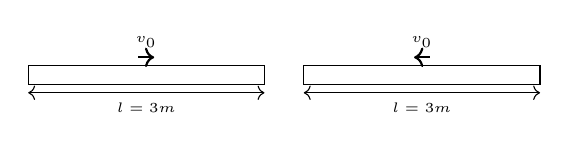
\begin{tikzpicture}
      \draw (0,0) rectangle (3,0.25);
      \draw[<->] (0,-0.1) -- (3,-0.1) node [midway, below] {\tiny $l=3m$};
      \draw[->,thick] (1.4,0.35) -- (1.6,0.35) node [midway, above] {\tiny $v_0$};
      \draw[<->] (3.5,-0.1) -- (6.5,-0.1) node [midway, below] {\tiny $l=3m$};
      \draw[<-,thick] (4.9,0.35) -- (5.1,0.35) node [midway, above] {\tiny $v_0$};
      \draw (3.5,0) rectangle (6.5,0.25);
    \end{tikzpicture}
  \end{block}
  %\pause
  \centering
  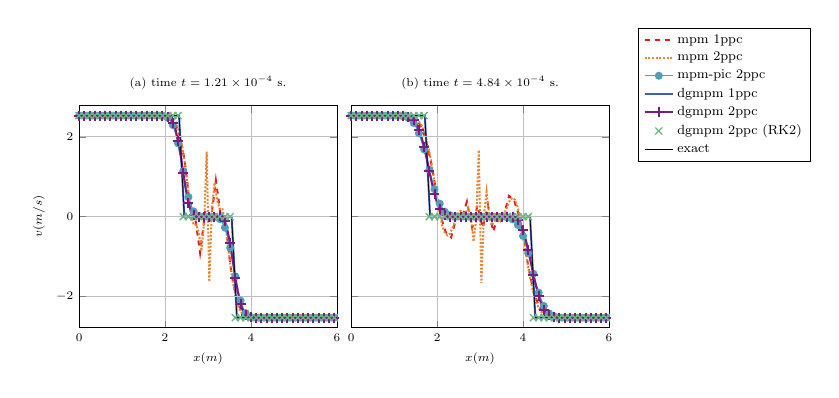
\begin{tikzpicture}[scale=.6]
\begin{groupplot}[group style={group size=2 by 1,
ylabels at=edge left, yticklabels at=edge left,horizontal sep=2.ex,
vertical sep=2ex,xticklabels at=edge bottom,xlabels at=edge bottom},
ymajorgrids=true,xmajorgrids=true,enlargelimits=0,xmin=0.,xmax=6.,xlabel=$x (m)$,
axis on top,scale only axis,width=0.45\linewidth
]
\nextgroupplot[ylabel=$v (m/s)$,ymin=-2.785033259480085,ymax=2.785033259480085,title={(a) time $t = 1.21\times 10^{-4} $ s.},]
\addplot[Red,dashed,mark=none,very thick,mark size=3pt,mark repeat=2] coordinates{(0.0,2.5318484177091665) (0.12244897959183673,2.5318484177091665) (0.24489795918367346,2.531848417709166) (0.36734693877551017,2.531848417709166) (0.4897959183673469,2.5318484177091656) (0.6122448979591837,2.5318484177091665) (0.7346938775510203,2.531848417709167) (0.8571428571428571,2.5318484177091665) (0.9795918367346939,2.5318484177091665) (1.1020408163265305,2.5318484177091665) (1.2244897959183674,2.5318484177091665) (1.346938775510204,2.5318484177091665) (1.4693877551020407,2.5318484177091665) (1.5918367346938775,2.5318484177091665) (1.7142857142857142,2.5318484177091665) (1.836734693877551,2.531684227710154) (1.9591836734693877,2.528883339491711) (2.0816326530612246,2.5069977784469075) (2.204081632653061,2.405451093175476) (2.326530612244898,2.0843630627542513) (2.4489795918367347,1.4571958994685654) (2.571428571428571,0.3681332942558399) (2.693877551020408,0.03859430800310576) (2.816326530612245,-0.9060776804312415) (2.9387755102040813,0.15497604259705183) (3.061224489795918,-0.15497604259704956) (3.183673469387755,0.9060776804312402) (3.306122448979592,-0.038594308003106204) (3.4285714285714284,-0.3681332942558391) (3.5510204081632653,-1.4571958994685674) (3.673469387755102,-2.084363062754252) (3.7959183673469385,-2.4054510931754756) (3.9183673469387754,-2.506997778446907) (4.040816326530612,-2.5288833394917107) (4.163265306122449,-2.531684227710154) (4.285714285714286,-2.5318484177091665) (4.408163265306122,-2.5318484177091665) (4.530612244897959,-2.5318484177091665) (4.653061224489796,-2.5318484177091665) (4.775510204081632,-2.5318484177091665) (4.8979591836734695,-2.5318484177091665) (5.020408163265306,-2.5318484177091665) (5.142857142857142,-2.5318484177091665) (5.26530612244898,-2.5318484177091665) (5.387755102040816,-2.5318484177091665) (5.5102040816326525,-2.5318484177091665) (5.63265306122449,-2.5318484177091665) (5.755102040816326,-2.5318484177091665) (5.877551020408163,-2.5318484177091665) (6.0,-2.5318484177091665) };
\addplot[Orange,densely dotted,mark=none,very thick,mark size=3pt,mark repeat=2] coordinates{(0.0,2.5318484177091665) (0.06060606060606061,2.5318484177091665) (0.12121212121212122,2.5318484177091665) (0.18181818181818182,2.5318484177091665) (0.24242424242424243,2.5318484177091665) (0.30303030303030304,2.5318484177091665) (0.36363636363636365,2.5318484177091665) (0.42424242424242425,2.5318484177091665) (0.48484848484848486,2.5318484177091665) (0.5454545454545454,2.5318484177091665) (0.6060606060606061,2.5318484177091665) (0.6666666666666667,2.531848417709167) (0.7272727272727273,2.531848417709167) (0.7878787878787878,2.5318484177091665) (0.8484848484848485,2.5318484177091665) (0.9090909090909092,2.5318484177091674) (0.9696969696969697,2.5318484177091665) (1.0303030303030303,2.5318484177091665) (1.0909090909090908,2.5318484177091656) (1.1515151515151516,2.5318484177091665) (1.2121212121212122,2.5318484177091665) (1.2727272727272727,2.5318484177091665) (1.3333333333333335,2.5318484177091656) (1.393939393939394,2.531848417709166) (1.4545454545454546,2.5318484177091665) (1.5151515151515151,2.5318484177091656) (1.5757575757575757,2.5318484177091665) (1.6363636363636365,2.531848417709167) (1.696969696969697,2.5318484177091665) (1.7575757575757576,2.5318484177091665) (1.8181818181818183,2.5318020034751854) (1.878787878787879,2.5317091750072236) (1.9393939393939394,2.5307501424302727) (2.0,2.5289249057443333) (2.0606060606060606,2.5201129167796545) (2.121212121212121,2.504314175536237) (2.1818181818181817,2.4573457248537327) (2.2424242424242427,2.379207564732142) (2.303030303030303,2.2185258725100665) (2.3636363636363638,1.975300648187503) (2.4242424242424243,1.625621223269172) (2.484848484848485,1.1694875977550743) (2.5454545454545454,0.6521580355962723) (2.606060606060606,0.07363253679276927) (2.666666666666667,-0.20959340058418097) (2.7272727272727275,-0.1975197765345734) (2.787878787878788,-0.4134073094303823) (2.8484848484848486,-0.8572559992716083) (2.909090909090909,-0.17642315371687442) (2.9696969696969697,1.6290912272338196) (3.0303030303030303,-1.6290912272338194) (3.090909090909091,0.17642315371686795) (3.1515151515151514,0.8572559992716065) (3.2121212121212124,0.41340730943038484) (3.272727272727273,0.19751977653457933) (3.3333333333333335,0.20959340058418124) (3.393939393939394,-0.07363253679276877) (3.4545454545454546,-0.6521580355962722) (3.515151515151515,-1.1694875977550738) (3.5757575757575757,-1.6256212232691716) (3.6363636363636367,-1.9753006481875028) (3.6969696969696972,-2.2185258725100656) (3.757575757575758,-2.3792075647321425) (3.8181818181818183,-2.457345724853733) (3.878787878787879,-2.5043141755362366) (3.9393939393939394,-2.520112916779654) (4.0,-2.528924905744333) (4.0606060606060606,-2.5307501424302727) (4.121212121212121,-2.5317091750072236) (4.181818181818182,-2.531802003475186) (4.242424242424242,-2.5318484177091665) (4.303030303030303,-2.5318484177091665) (4.363636363636363,-2.5318484177091665) (4.424242424242425,-2.5318484177091665) (4.484848484848485,-2.5318484177091665) (4.545454545454546,-2.5318484177091665) (4.606060606060606,-2.5318484177091665) (4.666666666666667,-2.5318484177091665) (4.7272727272727275,-2.5318484177091665) (4.787878787878788,-2.5318484177091665) (4.848484848484849,-2.5318484177091665) (4.909090909090909,-2.5318484177091665) (4.96969696969697,-2.5318484177091665) (5.03030303030303,-2.5318484177091665) (5.090909090909091,-2.5318484177091665) (5.151515151515151,-2.5318484177091665) (5.212121212121212,-2.5318484177091665) (5.2727272727272725,-2.5318484177091665) (5.333333333333334,-2.5318484177091665) (5.3939393939393945,-2.5318484177091665) (5.454545454545455,-2.5318484177091665) (5.515151515151516,-2.5318484177091665) (5.575757575757576,-2.5318484177091665) (5.636363636363637,-2.5318484177091665) (5.696969696969697,-2.5318484177091665) (5.757575757575758,-2.5318484177091665) (5.818181818181818,-2.5318484177091665) (5.878787878787879,-2.5318484177091665) (5.9393939393939394,-2.5318484177091665) (6.0,-2.5318484177091665) };
\addplot[Duck,solid,mark=*,thick,mark size=2pt,mark repeat=2] coordinates{(0.0,2.5318484177091665) (0.06060606060606061,2.5318484177091665) (0.12121212121212122,2.5318484177091665) (0.18181818181818182,2.5318484177091665) (0.24242424242424243,2.531848417709166) (0.30303030303030304,2.531848417709166) (0.36363636363636365,2.531848417709166) (0.42424242424242425,2.531848417709166) (0.48484848484848486,2.531848417709166) (0.5454545454545454,2.531848417709166) (0.6060606060606061,2.531848417709166) (0.6666666666666667,2.531848417709166) (0.7272727272727273,2.531848417709166) (0.7878787878787878,2.531848417709166) (0.8484848484848485,2.531848417709166) (0.9090909090909092,2.531848417709166) (0.9696969696969697,2.531848417709166) (1.0303030303030303,2.5318484177091656) (1.0909090909090908,2.531848417709166) (1.1515151515151516,2.531848417709166) (1.2121212121212122,2.5318484177091665) (1.2727272727272727,2.5318484177091665) (1.3333333333333335,2.5318484177091665) (1.393939393939394,2.5318484177091665) (1.4545454545454546,2.5318484177091665) (1.5151515151515151,2.5318484177091665) (1.5757575757575757,2.5318484177091665) (1.6363636363636365,2.5318484177091665) (1.696969696969697,2.5318484177091665) (1.7575757575757576,2.5318484177091665) (1.8181818181818183,2.5314767282665054) (1.878787878787879,2.530733349381183) (1.9393939393939394,2.5251504222424406) (2.0,2.5147279468502757) (2.0606060606060606,2.4791562919092076) (2.121212121212121,2.418435457419236) (2.1818181818181817,2.293184610622088) (2.2424242424242427,2.1034037515177637) (2.303030303030303,1.8369856040367076) (2.3636363636363638,1.4939301681789166) (2.4242424242424243,1.1415549355096852) (2.484848484848485,0.7798599060290146) (2.5454545454545454,0.49089965505724753) (2.606060606060606,0.2746741825943853) (2.666666666666667,0.13130830787569914) (2.7272727272727275,0.060802030901189776) (2.787878787878788,0.019549701006694658) (2.8484848484848486,0.007551318192214021) (2.909090909090909,0.0011640950887300435) (2.9696969696969697,0.00038803169624276515) (3.0303030303030303,-0.0003880316962443448) (3.090909090909091,-0.0011640950887312836) (3.1515151515151514,-0.007551318192214904) (3.2121212121212124,-0.019549701006695293) (3.272727272727273,-0.0608020309011897) (3.3333333333333335,-0.13130830787569833) (3.393939393939394,-0.2746741825943841) (3.4545454545454546,-0.49089965505724675) (3.515151515151515,-0.7798599060290139) (3.5757575757575757,-1.141554935509685) (3.6363636363636367,-1.4939301681789163) (3.6969696969696972,-1.8369856040367067) (3.757575757575758,-2.1034037515177646) (3.8181818181818183,-2.2931846106220877) (3.878787878787879,-2.418435457419236) (3.9393939393939394,-2.479156291909208) (4.0,-2.514727946850276) (4.0606060606060606,-2.52515042224244) (4.121212121212121,-2.5307333493811837) (4.181818181818182,-2.5314767282665054) (4.242424242424242,-2.5318484177091665) (4.303030303030303,-2.5318484177091665) (4.363636363636363,-2.5318484177091665) (4.424242424242425,-2.5318484177091665) (4.484848484848485,-2.5318484177091665) (4.545454545454546,-2.5318484177091665) (4.606060606060606,-2.5318484177091665) (4.666666666666667,-2.5318484177091665) (4.7272727272727275,-2.5318484177091665) (4.787878787878788,-2.5318484177091665) (4.848484848484849,-2.5318484177091665) (4.909090909090909,-2.5318484177091665) (4.96969696969697,-2.5318484177091665) (5.03030303030303,-2.5318484177091665) (5.090909090909091,-2.5318484177091665) (5.151515151515151,-2.5318484177091665) (5.212121212121212,-2.5318484177091665) (5.2727272727272725,-2.5318484177091665) (5.333333333333334,-2.5318484177091665) (5.3939393939393945,-2.5318484177091665) (5.454545454545455,-2.5318484177091665) (5.515151515151516,-2.5318484177091665) (5.575757575757576,-2.5318484177091665) (5.636363636363637,-2.5318484177091665) (5.696969696969697,-2.5318484177091665) (5.757575757575758,-2.5318484177091665) (5.818181818181818,-2.5318484177091665) (5.878787878787879,-2.5318484177091665) (5.9393939393939394,-2.5318484177091665) (6.0,-2.5318484177091665) };
\addplot[Blue,solid,mark=none,very thick,mark size=3pt,mark repeat=2] coordinates{(0.0,2.531848417709167) (0.12244897959183673,2.5318484177091656) (0.24489795918367346,2.531848417709166) (0.36734693877551017,2.5318484177091665) (0.4897959183673469,2.531848417709166) (0.6122448979591837,2.531848417709166) (0.7346938775510203,2.531848417709166) (0.8571428571428571,2.531848417709166) (0.9795918367346939,2.531848417709166) (1.1020408163265305,2.531848417709166) (1.2244897959183674,2.5318484177091656) (1.346938775510204,2.531848417709166) (1.4693877551020407,2.531848417709166) (1.5918367346938775,2.5318484177091665) (1.7142857142857142,2.531848417709166) (1.836734693877551,2.531848417709167) (1.9591836734693877,2.5318484177091665) (2.0816326530612246,2.5318484177091665) (2.204081632653061,2.5318484177091665) (2.326530612244898,2.5318484177091665) (2.4489795918367347,0.0) (2.571428571428571,-1.131824441720173e-15) (2.693877551020408,3.772748139067242e-16) (2.816326530612245,-3.944304526105059e-31) (2.9387755102040813,7.545496278134482e-16) (3.061224489795918,-1.131824441720173e-15) (3.183673469387755,3.772748139067241e-16) (3.306122448979592,3.772748139067244e-16) (3.4285714285714284,7.545496278134485e-16) (3.5510204081632653,2.220446049250313e-16) (3.673469387755102,-2.5318484177091665) (3.7959183673469385,-2.531848417709166) (3.9183673469387754,-2.531848417709166) (4.040816326530612,-2.531848417709167) (4.163265306122449,-2.531848417709166) (4.285714285714286,-2.5318484177091656) (4.408163265306122,-2.531848417709167) (4.530612244897959,-2.5318484177091665) (4.653061224489796,-2.531848417709166) (4.775510204081632,-2.531848417709167) (4.8979591836734695,-2.5318484177091665) (5.020408163265306,-2.531848417709167) (5.142857142857142,-2.531848417709167) (5.26530612244898,-2.531848417709167) (5.387755102040816,-2.531848417709167) (5.5102040816326525,-2.531848417709167) (5.63265306122449,-2.5318484177091665) (5.755102040816326,-2.531848417709166) (5.877551020408163,-2.531848417709167) (6.0,-2.5318484177091665) };
\addplot[Purple,solid,mark=+,very thick,mark size=3pt,mark repeat=2] coordinates{(0.0,2.531848417709166) (0.06060606060606061,2.531848417709166) (0.12121212121212122,2.531848417709166) (0.18181818181818182,2.531848417709166) (0.24242424242424243,2.5318484177091656) (0.30303030303030304,2.5318484177091656) (0.36363636363636365,2.5318484177091656) (0.42424242424242425,2.5318484177091656) (0.48484848484848486,2.5318484177091656) (0.5454545454545454,2.531848417709165) (0.6060606060606061,2.531848417709165) (0.6666666666666667,2.531848417709165) (0.7272727272727273,2.531848417709165) (0.7878787878787878,2.531848417709165) (0.8484848484848485,2.531848417709165) (0.9090909090909092,2.5318484177091647) (0.9696969696969697,2.5318484177091647) (1.0303030303030303,2.5318484177091647) (1.0909090909090908,2.5318484177091647) (1.1515151515151516,2.531848417709165) (1.2121212121212122,2.531848417709165) (1.2727272727272727,2.531848417709165) (1.3333333333333335,2.531848417709165) (1.393939393939394,2.531848417709165) (1.4545454545454546,2.531848417709165) (1.5151515151515151,2.5318484177091656) (1.5757575757575757,2.5318484177091656) (1.6363636363636365,2.531848417709166) (1.696969696969697,2.531848417709166) (1.7575757575757576,2.531848417709166) (1.8181818181818183,2.5317555939571394) (1.878787878787879,2.5315699464530863) (1.9393939393939394,2.529300921403548) (2.0,2.5251960488139282) (2.0606060606060606,2.502983668745643) (2.121212121212121,2.4672568379656363) (2.1818181818181817,2.3558296271378385) (2.2424242424242427,2.199909152499134) (2.303030303030303,1.8955358394101423) (2.3636363636363638,1.5350380403392951) (2.4242424242424243,1.0913569359704094) (2.484848484848485,0.6616953448225573) (2.5454545454545454,0.35041226238060424) (2.606060606060606,0.11398111608931762) (2.666666666666667,0.037623711953108305) (2.7272727272727275,-0.006618739561512254) (2.787878787878788,-0.0024042733543885486) (2.8484848484848486,-0.0017885136987410197) (2.909090909090909,-0.0001900946309221662) (2.9696969696969697,4.075039583706578e-05) (3.0303030303030303,-4.075039583690026e-05) (3.090909090909091,0.000190094630922048) (3.1515151515151514,0.001788513698741276) (3.2121212121212124,0.0024042733543890842) (3.272727272727273,0.006618739561513227) (3.3333333333333335,-0.03762371195310714) (3.393939393939394,-0.11398111608931744) (3.4545454545454546,-0.35041226238060363) (3.515151515151515,-0.6616953448225579) (3.5757575757575757,-1.09135693597041) (3.6363636363636367,-1.535038040339297) (3.6969696969696972,-1.8955358394101425) (3.757575757575758,-2.199909152499135) (3.8181818181818183,-2.3558296271378385) (3.878787878787879,-2.4672568379656363) (3.9393939393939394,-2.502983668745643) (4.0,-2.5251960488139282) (4.0606060606060606,-2.5293009214035473) (4.121212121212121,-2.5315699464530863) (4.181818181818182,-2.5317555939571394) (4.242424242424242,-2.531848417709166) (4.303030303030303,-2.531848417709166) (4.363636363636363,-2.531848417709166) (4.424242424242425,-2.531848417709166) (4.484848484848485,-2.531848417709166) (4.545454545454546,-2.531848417709166) (4.606060606060606,-2.531848417709166) (4.666666666666667,-2.531848417709166) (4.7272727272727275,-2.531848417709166) (4.787878787878788,-2.531848417709166) (4.848484848484849,-2.531848417709166) (4.909090909090909,-2.531848417709166) (4.96969696969697,-2.531848417709166) (5.03030303030303,-2.531848417709166) (5.090909090909091,-2.531848417709166) (5.151515151515151,-2.531848417709166) (5.212121212121212,-2.531848417709166) (5.2727272727272725,-2.531848417709166) (5.333333333333334,-2.531848417709166) (5.3939393939393945,-2.531848417709166) (5.454545454545455,-2.531848417709166) (5.515151515151516,-2.531848417709166) (5.575757575757576,-2.531848417709166) (5.636363636363637,-2.531848417709166) (5.696969696969697,-2.531848417709166) (5.757575757575758,-2.531848417709166) (5.818181818181818,-2.531848417709166) (5.878787878787879,-2.531848417709166) (5.9393939393939394,-2.531848417709166) (6.0,-2.5318484177091665) };
\addplot[Green,only marks,mark=x,thick,mark size=3pt,mark repeat=2] coordinates{(0.0,2.531848417709166) (0.06060606060606061,2.531848417709166) (0.12121212121212122,2.531848417709166) (0.18181818181818182,2.531848417709166) (0.24242424242424243,2.5318484177091665) (0.30303030303030304,2.5318484177091665) (0.36363636363636365,2.5318484177091656) (0.42424242424242425,2.5318484177091656) (0.48484848484848486,2.5318484177091665) (0.5454545454545454,2.5318484177091665) (0.6060606060606061,2.531848417709165) (0.6666666666666667,2.5318484177091656) (0.7272727272727273,2.531848417709166) (0.7878787878787878,2.531848417709166) (0.8484848484848485,2.5318484177091656) (0.9090909090909092,2.5318484177091656) (0.9696969696969697,2.5318484177091665) (1.0303030303030303,2.5318484177091665) (1.0909090909090908,2.5318484177091647) (1.1515151515151516,2.531848417709165) (1.2121212121212122,2.531848417709166) (1.2727272727272727,2.531848417709166) (1.3333333333333335,2.5318484177091647) (1.393939393939394,2.5318484177091647) (1.4545454545454546,2.5318484177091665) (1.5151515151515151,2.5318484177091665) (1.5757575757575757,2.531848417709166) (1.6363636363636365,2.531848417709166) (1.696969696969697,2.531848417709166) (1.7575757575757576,2.531848417709166) (1.8181818181818183,2.531848417709166) (1.878787878787879,2.531848417709166) (1.9393939393939394,2.531848417709166) (2.0,2.531848417709166) (2.0606060606060606,2.5318484177091656) (2.121212121212121,2.531848417709166) (2.1818181818181817,2.5318484177091665) (2.2424242424242427,2.531848417709166) (2.303030303030303,2.5318484177091665) (2.3636363636363638,2.5318484177091665) (2.4242424242424243,7.771561172376108e-16) (2.484848484848485,-2.1094237467877935e-15) (2.5454545454545454,-2.4980018054065835e-16) (2.606060606060606,-1.0824674490095235e-15) (2.666666666666667,8.52730145933733e-16) (2.7272727272727275,8.332007357698796e-16) (2.787878787878788,-6.636926385046085e-16) (2.8484848484848486,-6.685749910455732e-16) (2.909090909090909,-9.666384036373804e-17) (2.9696969696969697,2.734954664404533e-16) (3.0303030303030303,-9.789796087117351e-17) (3.090909090909091,9.860763805712963e-16) (3.1515151515151514,-5.850647289005321e-16) (3.2121212121212124,-3.585610702627896e-17) (3.272727272727273,8.518216860046792e-17) (3.3333333333333335,-1.2838500279050285e-16) (3.393939393939394,1.7783669840585248e-16) (3.4545454545454546,8.942088536749598e-17) (3.515151515151515,-9.992007221626425e-16) (3.5757575757575757,2.331468351712824e-15) (3.6363636363636367,-2.531848417709166) (3.6969696969696972,-2.5318484177091665) (3.757575757575758,-2.531848417709166) (3.8181818181818183,-2.5318484177091665) (3.878787878787879,-2.531848417709166) (3.9393939393939394,-2.5318484177091665) (4.0,-2.531848417709166) (4.0606060606060606,-2.531848417709166) (4.121212121212121,-2.531848417709166) (4.181818181818182,-2.531848417709166) (4.242424242424242,-2.5318484177091665) (4.303030303030303,-2.531848417709167) (4.363636363636363,-2.531848417709165) (4.424242424242425,-2.531848417709165) (4.484848484848485,-2.5318484177091665) (4.545454545454546,-2.5318484177091665) (4.606060606060606,-2.5318484177091665) (4.666666666666667,-2.5318484177091665) (4.7272727272727275,-2.5318484177091656) (4.787878787878788,-2.531848417709166) (4.848484848484849,-2.531848417709166) (4.909090909090909,-2.5318484177091665) (4.96969696969697,-2.531848417709166) (5.03030303030303,-2.5318484177091665) (5.090909090909091,-2.531848417709166) (5.151515151515151,-2.5318484177091665) (5.212121212121212,-2.531848417709166) (5.2727272727272725,-2.5318484177091665) (5.333333333333334,-2.531848417709166) (5.3939393939393945,-2.5318484177091665) (5.454545454545455,-2.531848417709166) (5.515151515151516,-2.5318484177091665) (5.575757575757576,-2.531848417709166) (5.636363636363637,-2.5318484177091665) (5.696969696969697,-2.531848417709166) (5.757575757575758,-2.5318484177091665) (5.818181818181818,-2.531848417709166) (5.878787878787879,-2.5318484177091665) (5.9393939393939394,-2.5318484177091665) (6.0,-2.5318484177091665) };
\addplot[black,solid,mark=pentagone*,thin,mark size=3pt,mark repeat=2] coordinates{(0.0,2.5318484177091665) (0.12244897959183673,2.5318484177091665) (0.24489795918367346,2.5318484177091665) (0.36734693877551017,2.5318484177091665) (0.4897959183673469,2.5318484177091665) (0.6122448979591837,2.5318484177091665) (0.7346938775510203,2.5318484177091665) (0.8571428571428571,2.5318484177091665) (0.9795918367346939,2.5318484177091665) (1.1020408163265305,2.5318484177091665) (1.2244897959183674,2.5318484177091665) (1.346938775510204,2.5318484177091665) (1.4693877551020407,2.5318484177091665) (1.5918367346938775,2.5318484177091665) (1.7142857142857142,2.5318484177091665) (1.836734693877551,2.5318484177091665) (1.9591836734693877,2.5318484177091665) (2.0816326530612246,2.5318484177091665) (2.204081632653061,2.5318484177091665) (2.326530612244898,2.5318484177091665) (2.4489795918367347,0.0) (2.571428571428571,0.0) (2.693877551020408,0.0) (2.816326530612245,0.0) (2.9387755102040813,0.0) (3.061224489795918,-0.0) (3.183673469387755,-0.0) (3.306122448979592,-0.0) (3.4285714285714284,-0.0) (3.5510204081632653,-0.0) (3.673469387755102,-2.5318484177091665) (3.7959183673469385,-2.5318484177091665) (3.9183673469387754,-2.5318484177091665) (4.040816326530612,-2.5318484177091665) (4.163265306122449,-2.5318484177091665) (4.285714285714286,-2.5318484177091665) (4.408163265306122,-2.5318484177091665) (4.530612244897959,-2.5318484177091665) (4.653061224489796,-2.5318484177091665) (4.775510204081632,-2.5318484177091665) (4.8979591836734695,-2.5318484177091665) (5.020408163265306,-2.5318484177091665) (5.142857142857142,-2.5318484177091665) (5.26530612244898,-2.5318484177091665) (5.387755102040816,-2.5318484177091665) (5.5102040816326525,-2.5318484177091665) (5.63265306122449,-2.5318484177091665) (5.755102040816326,-2.5318484177091665) (5.877551020408163,-2.5318484177091665) (6.0,-2.5318484177091665) };
\nextgroupplot[legend style={at={($(0.7,-0.35)+(5.9cm,8cm)$)},legend columns=1},ymin=-2.785033259480085,ymax=2.785033259480085,title={(b) time $t = 4.84\times 10^{-4} $ s.}]
\addplot[Red,dashed,mark=none,very thick,mark size=3pt,mark repeat=2] coordinates{(0.0,2.5318484177091665) (0.12244897959183673,2.531848417709167) (0.24489795918367346,2.531848417709166) (0.36734693877551017,2.531848417709166) (0.4897959183673469,2.531848417709165) (0.6122448979591837,2.5318483984539664) (0.7346938775510203,2.5318477659475827) (0.8571428571428571,2.5318378383698152) (0.9795918367346939,2.531738909821285) (1.1020408163265305,2.5310376550966116) (1.2244897959183674,2.5272846058424623) (1.346938775510204,2.511582995381506) (1.4693877551020407,2.4591766365643473) (1.5918367346938775,2.3181168751417087) (1.7142857142857142,2.0117581239436237) (1.836734693877551,1.477297258708373) (1.9591836734693877,0.7554822113442998) (2.0816326530612246,0.010684165656105471) (2.204081632653061,-0.39396688397347013) (2.326530612244898,-0.5189112540071943) (2.4489795918367347,-0.020711514080181737) (2.571428571428571,-0.04925338946186149) (2.693877551020408,0.3772292528240989) (2.816326530612245,-0.28486682427919574) (2.9387755102040813,0.279534610825791) (3.061224489795918,-0.2795346108257906) (3.183673469387755,0.2848668242791922) (3.306122448979592,-0.37722925282409936) (3.4285714285714284,0.04925338946185971) (3.5510204081632653,0.020711514080185872) (3.673469387755102,0.518911254007197) (3.7959183673469385,0.3939668839734717) (3.9183673469387754,-0.010684165656106692) (4.040816326530612,-0.7554822113442974) (4.163265306122449,-1.477297258708377) (4.285714285714286,-2.011758123943624) (4.408163265306122,-2.3181168751417087) (4.530612244897959,-2.459176636564347) (4.653061224489796,-2.511582995381506) (4.775510204081632,-2.5272846058424627) (4.8979591836734695,-2.5310376550966107) (5.020408163265306,-2.531738909821284) (5.142857142857142,-2.531837838369815) (5.26530612244898,-2.5318477659475827) (5.387755102040816,-2.5318483984539664) (5.5102040816326525,-2.5318484177091665) (5.63265306122449,-2.5318484177091665) (5.755102040816326,-2.5318484177091665) (5.877551020408163,-2.5318484177091665) (6.0,-2.5318484177091665) };
\addplot[Orange,densely dotted,mark=none,very thick,mark size=3pt,mark repeat=2] coordinates{(0.0,2.5318484177091665) (0.06060606060606061,2.5318484177091665) (0.12121212121212122,2.5318484177091665) (0.18181818181818182,2.5318484177091665) (0.24242424242424243,2.5318484177091665) (0.30303030303030304,2.5318484177091665) (0.36363636363636365,2.5318484177091665) (0.42424242424242425,2.5318484177091665) (0.48484848484848486,2.5318484177091665) (0.5454545454545454,2.5318484177091665) (0.6060606060606061,2.5318484151568073) (0.6666666666666667,2.531848410052089) (0.7272727272727273,2.5318483062561463) (0.7878787878787878,2.5318481037689806) (0.8484848484848485,2.5318461134959485) (0.9090909090909092,2.5318423354370503) (0.9696969696969697,2.531818445166049) (1.0303030303030303,2.531774442682947) (1.0909090909090908,2.531573501160723) (1.1515151515151516,2.531215620599377) (1.2121212121212122,2.529959996602834) (1.2727272727272727,2.5278066291710957) (1.3333333333333335,2.5217797302083578) (1.393939393939394,2.5118792997146255) (1.4545454545454546,2.489236665383997) (1.5151515151515151,2.4538518272164733) (1.5757575757575757,2.3867144217459435) (1.6363636363636365,2.2878244489724064) (1.696969696969697,2.1309266174919825) (1.7575757575757576,1.9160209273046755) (1.8181818181818183,1.6307338302347996) (1.878787878787879,1.2750653262823581) (1.9393939393939394,0.8846124649872573) (2.0,0.45937524634950305) (2.0606060606060606,0.08727763903668462) (2.121212121212121,-0.23168035695119626) (2.1818181818181817,-0.4175483709794803) (2.2424242424242427,-0.4703264030481671) (2.303030303030303,-0.41875637304195895) (2.3636363636363638,-0.26283828096085887) (2.4242424242424243,-0.0954921221874162) (2.484848484848485,0.08328210327836835) (2.5454545454545454,0.14407234790709328) (2.606060606060606,0.08687861169875953) (2.666666666666667,0.11137418504956392) (2.7272727272727275,0.21755906795950974) (2.787878787878788,-0.02803136011717798) (2.8484848484848486,-0.6253970991805003) (2.909090909090909,-0.06009787210682943) (2.9696969696969697,1.6678663211038354) (3.0303030303030303,-1.6678663211038323) (3.090909090909091,0.06009787210682655) (3.1515151515151514,0.6253970991805009) (3.2121212121212124,0.028031360117178453) (3.272727272727273,-0.21755906795950636) (3.3333333333333335,-0.1113741850495652) (3.393939393939394,-0.08687861169876046) (3.4545454545454546,-0.14407234790709447) (3.515151515151515,-0.08328210327836953) (3.5757575757575757,0.09549212218741482) (3.6363636363636367,0.26283828096085826) (3.6969696969696972,0.4187563730419601) (3.757575757575758,0.47032640304816764) (3.8181818181818183,0.4175483709794797) (3.878787878787879,0.2316803569511961) (3.9393939393939394,-0.0872776390366839) (4.0,-0.4593752463495025) (4.0606060606060606,-0.8846124649872572) (4.121212121212121,-1.275065326282357) (4.181818181818182,-1.6307338302348002) (4.242424242424242,-1.916020927304675) (4.303030303030303,-2.130926617491981) (4.363636363636363,-2.2878244489724056) (4.424242424242425,-2.3867144217459453) (4.484848484848485,-2.4538518272164747) (4.545454545454546,-2.4892366653839972) (4.606060606060606,-2.5118792997146255) (4.666666666666667,-2.5217797302083578) (4.7272727272727275,-2.5278066291710943) (4.787878787878788,-2.5299599966028334) (4.848484848484849,-2.5312156205993763) (4.909090909090909,-2.5315735011607234) (4.96969696969697,-2.5317744426829467) (5.03030303030303,-2.5318184451660493) (5.090909090909091,-2.53184233543705) (5.151515151515151,-2.531846113495948) (5.212121212121212,-2.53184810376898) (5.2727272727272725,-2.5318483062561463) (5.333333333333334,-2.531848410052089) (5.3939393939393945,-2.5318484151568073) (5.454545454545455,-2.5318484177091665) (5.515151515151516,-2.5318484177091665) (5.575757575757576,-2.5318484177091665) (5.636363636363637,-2.5318484177091665) (5.696969696969697,-2.5318484177091665) (5.757575757575758,-2.5318484177091665) (5.818181818181818,-2.5318484177091665) (5.878787878787879,-2.5318484177091665) (5.9393939393939394,-2.5318484177091665) (6.0,-2.5318484177091665) };
\addplot[Duck,solid,mark=*,thick,mark size=2pt,mark repeat=2] coordinates{(0.0,2.531848417709166) (0.06060606060606061,2.531848417709166) (0.12121212121212122,2.531848417709166) (0.18181818181818182,2.531848417709166) (0.24242424242424243,2.531848417709166) (0.30303030303030304,2.531848417709166) (0.36363636363636365,2.531848417709166) (0.42424242424242425,2.531848417709166) (0.48484848484848486,2.531848417709166) (0.5454545454545454,2.531848417709166) (0.6060606060606061,2.531848322218527) (0.6666666666666667,2.5318481312372487) (0.7272727272727273,2.5318451768738073) (0.7878787878787878,2.531839459128202) (0.8484848484848485,2.5317972741399446) (0.9090909090909092,2.531718621909035) (0.9696969696969697,2.531349985135261) (1.0303030303030303,2.530691363818622) (1.0909090909090908,2.528487041474035) (1.1515151515151516,2.5247370181015003) (1.2121212121212122,2.5151819070173778) (1.2727272727272727,2.499821708221668) (1.3333333333333335,2.4687849694057875) (1.393939393939394,2.4220716905697377) (1.4545454545454546,2.3450324107320544) (1.5151515151515151,2.2376671298927375) (1.5757575757575757,2.0899010681921935) (1.6363636363636365,1.9017342256304213) (1.696969696969697,1.6815563242811924) (1.7575757575757576,1.4293673641445055) (1.8181818181818183,1.1742121642120082) (1.878787878787879,0.9160907244837013) (1.9393939393939394,0.6865647991400854) (2.0,0.4856343881811611) (2.0606060606060606,0.32603252055315013) (2.121212121212121,0.2077591962560531) (2.1818181818181817,0.12249073841136798) (2.2424242424242427,0.0702271470190948) (2.303030303030303,0.03551770611448978) (2.3636363636363638,0.01836241569755198) (2.4242424242424243,0.007729710698309033) (2.484848484848485,0.003619591116760991) (2.5454545454545454,0.0012158346463164134) (2.606060606060606,0.0005184412869753138) (2.666666666666667,0.00013011416411164403) (2.7272727272727275,5.085327772540678e-05) (2.787878787878788,8.496748645186023e-06) (2.8484848484848486,3.0445768709820515e-06) (2.909090909090909,2.3886823801310813e-07) (2.9696969696969697,7.962274627921281e-08) (3.0303030303030303,-7.96227454470489e-08) (3.090909090909091,-2.388682371656764e-07) (3.1515151515151514,-3.044576870427015e-06) (3.2121212121212124,-8.496748645231104e-06) (3.272727272727273,-5.0853277725753164e-05) (3.3333333333333335,-0.00013011416411199333) (3.393939393939394,-0.0005184412869758035) (3.4545454545454546,-0.0012158346463171834) (3.515151515151515,-0.0036195911167619375) (3.5757575757575757,-0.007729710698310062) (3.6363636363636367,-0.018362415697552956) (3.6969696969696972,-0.0355177061144906) (3.757575757575758,-0.07022714701909577) (3.8181818181818183,-0.12249073841136837) (3.878787878787879,-0.2077591962560532) (3.9393939393939394,-0.32603252055315) (4.0,-0.4856343881811607) (4.0606060606060606,-0.686564799140085) (4.121212121212121,-0.9160907244837007) (4.181818181818182,-1.1742121642120076) (4.242424242424242,-1.4293673641445048) (4.303030303030303,-1.6815563242811915) (4.363636363636363,-1.9017342256304213) (4.424242424242425,-2.089901068192196) (4.484848484848485,-2.2376671298927384) (4.545454545454546,-2.3450324107320544) (4.606060606060606,-2.4220716905697377) (4.666666666666667,-2.468784969405788) (4.7272727272727275,-2.499821708221668) (4.787878787878788,-2.515181907017378) (4.848484848484849,-2.5247370181015008) (4.909090909090909,-2.528487041474035) (4.96969696969697,-2.530691363818622) (5.03030303030303,-2.531349985135261) (5.090909090909091,-2.5317186219090355) (5.151515151515151,-2.5317972741399446) (5.212121212121212,-2.5318394591282023) (5.2727272727272725,-2.5318451768738073) (5.333333333333334,-2.5318481312372496) (5.3939393939393945,-2.5318483222185275) (5.454545454545455,-2.5318484177091665) (5.515151515151516,-2.5318484177091665) (5.575757575757576,-2.5318484177091665) (5.636363636363637,-2.5318484177091665) (5.696969696969697,-2.5318484177091665) (5.757575757575758,-2.5318484177091665) (5.818181818181818,-2.5318484177091665) (5.878787878787879,-2.5318484177091665) (5.9393939393939394,-2.5318484177091665) (6.0,-2.5318484177091665) };
\addplot[Blue,solid,mark=none,very thick,mark size=3pt,mark repeat=2] coordinates{(0.0,2.5318484177091642) (0.12244897959183673,2.531848417709168) (0.24489795918367346,2.5318484177091647) (0.36734693877551017,2.531848417709165) (0.4897959183673469,2.531848417709166) (0.6122448979591837,2.531848417709166) (0.7346938775510203,2.531848417709166) (0.8571428571428571,2.531848417709167) (0.9795918367346939,2.531848417709166) (1.1020408163265305,2.531848417709166) (1.2244897959183674,2.5318484177091665) (1.346938775510204,2.531848417709166) (1.4693877551020407,2.531848417709166) (1.5918367346938775,2.531848417709166) (1.7142857142857142,2.531848417709166) (1.836734693877551,-6.661338147750939e-16) (1.9591836734693877,-2.485693488365377e-15) (2.0816326530612246,6.877352318701104e-16) (2.204081632653061,-5.9164567891575885e-31) (2.326530612244898,-3.7727481390672426e-16) (2.4489795918367347,3.944304526105059e-31) (2.571428571428571,1.1318244417201724e-15) (2.693877551020408,-5.9164567891575885e-31) (2.816326530612245,1.1318244417201723e-15) (2.9387755102040813,-3.944304526105059e-31) (3.061224489795918,-7.888609052210118e-31) (3.183673469387755,-3.772748139067248e-16) (3.306122448979592,2.2636488834403473e-15) (3.4285714285714284,-1.886374069533621e-15) (3.5510204081632653,2.1084186744586528e-15) (3.673469387755102,-9.981956498334958e-16) (3.7959183673469385,3.104604179633854e-16) (3.9183673469387754,-6.209208359267718e-16) (4.040816326530612,1.065010045776834e-15) (4.163265306122449,-1.5543122344752192e-15) (4.285714285714286,-2.531848417709166) (4.408163265306122,-2.531848417709167) (4.530612244897959,-2.5318484177091665) (4.653061224489796,-2.531848417709166) (4.775510204081632,-2.531848417709166) (4.8979591836734695,-2.531848417709166) (5.020408163265306,-2.5318484177091665) (5.142857142857142,-2.5318484177091665) (5.26530612244898,-2.531848417709166) (5.387755102040816,-2.5318484177091665) (5.5102040816326525,-2.531848417709167) (5.63265306122449,-2.531848417709167) (5.755102040816326,-2.531848417709167) (5.877551020408163,-2.531848417709167) (6.0,-2.531848417709168) };
\addplot[Purple,solid,mark=+,very thick,mark size=3pt,mark repeat=2] coordinates{(0.0,2.5318484177091625) (0.06060606060606061,2.5318484177091625) (0.12121212121212122,2.531848417709163) (0.18181818181818182,2.5318484177091634) (0.24242424242424243,2.5318484177091642) (0.30303030303030304,2.5318484177091642) (0.36363636363636365,2.531848417709164) (0.42424242424242425,2.531848417709164) (0.48484848484848486,2.531848417709164) (0.5454545454545454,2.531848417709164) (0.6060606060606061,2.5318484126044454) (0.6666666666666667,2.531848402395009) (0.7272727272727273,2.531848147159085) (0.7878787878787878,2.531847660509256) (0.8484848484848485,2.5318419112097796) (0.9090909090909092,2.5318314997267986) (0.9696969696969697,2.5317543577392794) (1.0303030303030303,2.531622226855984) (1.0909090909090908,2.5309352642773124) (1.1515151515151516,2.529827505784501) (1.2121212121212122,2.525544979109427) (1.2727272727272727,2.5190772040991836) (1.3333333333333335,2.49986453919368) (1.393939393939394,2.4728460487555486) (1.4545454545454546,2.4100439263485716) (1.5151515151515151,2.3283399292621993) (1.5757575757575757,2.178564100960003) (1.6363636363636365,1.999603107753429) (1.696969696969697,1.7412015276196833) (1.7575757575757576,1.4598954849283565) (1.8181818181818183,1.1436088819043788) (1.878787878787879,0.8326048422840917) (1.9393939393939394,0.5673667305700555) (2.0,0.3338637253193525) (2.0606060606060606,0.19081928650352253) (2.121212121212121,0.07885642245760108) (2.1818181818181817,0.035644258017509256) (2.2424242424242427,0.00543058051750829) (2.303030303030303,0.0012651237456281672) (2.3636363636363638,-0.0017052487095000686) (2.4242424242424243,-0.0006454300856452834) (2.484848484848485,-0.0002806339825737999) (2.5454545454545454,-6.316370952302816e-05) (2.606060606060606,1.1141267552461879e-05) (2.666666666666667,3.186617029754634e-06) (2.7272727272727275,2.224000786251848e-06) (2.787878787878788,2.458788272790853e-07) (2.8484848484848486,-4.858566390766534e-08) (2.909090909090909,-4.144118614765797e-09) (2.9696969696969697,-1.97507262108322e-09) (3.0303030303030303,1.9750719798293663e-09) (3.090909090909091,4.144118171518933e-09) (3.1515151515151514,4.8585664037513496e-08) (3.2121212121212124,-2.458788273706489e-07) (3.272727272727273,-2.2240007863010142e-06) (3.3333333333333335,-3.186617029443332e-06) (3.393939393939394,-1.114126755228617e-05) (3.4545454545454546,6.316370952276986e-05) (3.515151515151515,0.00028063398257326263) (3.5757575757575757,0.0006454300856452396) (3.6363636363636367,0.0017052487095003755) (3.6969696969696972,-0.001265123745628387) (3.757575757575758,-0.00543058051750882) (3.8181818181818183,-0.035644258017509936) (3.878787878787879,-0.0788564224576016) (3.9393939393939394,-0.19081928650352323) (4.0,-0.3338637253193546) (4.0606060606060606,-0.5673667305700569) (4.121212121212121,-0.8326048422840933) (4.181818181818182,-1.1436088819043795) (4.242424242424242,-1.4598954849283583) (4.303030303030303,-1.7412015276196846) (4.363636363636363,-1.9996031077534282) (4.424242424242425,-2.1785641009600054) (4.484848484848485,-2.328339929262201) (4.545454545454546,-2.410043926348574) (4.606060606060606,-2.4728460487555504) (4.666666666666667,-2.499864539193682) (4.7272727272727275,-2.519077204099186) (4.787878787878788,-2.525544979109429) (4.848484848484849,-2.5298275057845023) (4.909090909090909,-2.5309352642773137) (4.96969696969697,-2.531622226855986) (5.03030303030303,-2.5317543577392807) (5.090909090909091,-2.5318314997268) (5.151515151515151,-2.531841911209781) (5.212121212121212,-2.531847660509258) (5.2727272727272725,-2.5318481471590863) (5.333333333333334,-2.5318484023950107) (5.3939393939393945,-2.5318484126044476) (5.454545454545455,-2.531848417709166) (5.515151515151516,-2.531848417709166) (5.575757575757576,-2.531848417709166) (5.636363636363637,-2.531848417709166) (5.696969696969697,-2.531848417709166) (5.757575757575758,-2.531848417709166) (5.818181818181818,-2.531848417709166) (5.878787878787879,-2.531848417709166) (5.9393939393939394,-2.531848417709166) (6.0,-2.5318484177091665) };
\addplot[Green,only marks,mark=x,thick,mark size=3pt,mark repeat=2] coordinates{(0.0,2.531848417709165) (0.06060606060606061,2.5318484177091647) (0.12121212121212122,2.5318484177091647) (0.18181818181818182,2.531848417709165) (0.24242424242424243,2.5318484177091656) (0.30303030303030304,2.531848417709165) (0.36363636363636365,2.531848417709166) (0.42424242424242425,2.531848417709166) (0.48484848484848486,2.5318484177091642) (0.5454545454545454,2.531848417709164) (0.6060606060606061,2.531848417709166) (0.6666666666666667,2.531848417709166) (0.7272727272727273,2.5318484177091647) (0.7878787878787878,2.5318484177091647) (0.8484848484848485,2.5318484177091647) (0.9090909090909092,2.5318484177091647) (0.9696969696969697,2.531848417709166) (1.0303030303030303,2.531848417709166) (1.0909090909090908,2.531848417709166) (1.1515151515151516,2.531848417709166) (1.2121212121212122,2.5318484177091642) (1.2727272727272727,2.5318484177091642) (1.3333333333333335,2.5318484177091642) (1.393939393939394,2.5318484177091647) (1.4545454545454546,2.5318484177091647) (1.5151515151515151,2.5318484177091647) (1.5757575757575757,2.5318484177091647) (1.6363636363636365,2.5318484177091647) (1.696969696969697,2.5318484177091647) (1.7575757575757576,2.531848417709165) (1.8181818181818183,7.771561172376108e-16) (1.878787878787879,-2.1094237467877935e-15) (1.9393939393939394,-1.2428467441826863e-15) (2.0,-1.1544309311443312e-15) (2.0606060606060606,1.3696932073430366e-15) (2.121212121212121,1.2476189282507285e-15) (2.1818181818181817,-2.4419093580481207e-15) (2.2424242424242427,-2.085388408832536e-15) (2.303030303030303,1.2943623313739441e-17) (2.3636363636363638,-1.4657241520041104e-16) (2.4242424242424243,1.111119986946025e-15) (2.484848484848485,5.748108947575872e-16) (2.5454545454545454,-1.8234388364241851e-16) (2.606060606060606,-3.953741180943154e-16) (2.666666666666667,4.31804378727956e-16) (2.7272727272727275,4.995768751622078e-16) (2.787878787878788,5.150629572573582e-16) (2.8484848484848486,4.1631829663280534e-16) (2.909090909090909,-5.307314203763871e-16) (2.9696969696969697,-4.698658136034621e-17) (3.0303030303030303,3.4850435715606133e-16) (3.090909090909091,-2.1487556526938687e-16) (3.1515151515151514,7.267771520076887e-16) (3.2121212121212124,9.159508955058459e-16) (3.272727272727273,-3.4277021996705634e-16) (3.3333333333333335,-4.549822420364271e-16) (3.393939393939394,-5.717603789571251e-17) (3.4545454545454546,-4.301160061443877e-16) (3.515151515151515,2.732322650623179e-16) (3.5757575757575757,-4.500638911390337e-16) (3.6363636363636367,-3.9556189340519207e-16) (3.6969696969696972,-5.358193604849726e-16) (3.757575757575758,9.938081006729924e-16) (3.8181818181818183,1.0930091566906381e-15) (3.878787878787879,-7.515981825942874e-16) (3.9393939393939394,-6.238722811459393e-16) (4.0,3.77274813906722e-16) (4.0606060606060606,5.109036057933968e-16) (4.121212121212121,-1.221245327087674e-15) (4.181818181818182,2.553512956637855e-15) (4.242424242424242,-2.5318484177091656) (4.303030303030303,-2.5318484177091656) (4.363636363636363,-2.531848417709166) (4.424242424242425,-2.531848417709166) (4.484848484848485,-2.5318484177091665) (4.545454545454546,-2.5318484177091665) (4.606060606060606,-2.531848417709165) (4.666666666666667,-2.531848417709165) (4.7272727272727275,-2.5318484177091665) (4.787878787878788,-2.5318484177091665) (4.848484848484849,-2.5318484177091656) (4.909090909090909,-2.531848417709166) (4.96969696969697,-2.5318484177091656) (5.03030303030303,-2.5318484177091656) (5.090909090909091,-2.5318484177091665) (5.151515151515151,-2.5318484177091665) (5.212121212121212,-2.5318484177091665) (5.2727272727272725,-2.5318484177091665) (5.333333333333334,-2.5318484177091656) (5.3939393939393945,-2.531848417709166) (5.454545454545455,-2.531848417709166) (5.515151515151516,-2.5318484177091665) (5.575757575757576,-2.531848417709166) (5.636363636363637,-2.5318484177091665) (5.696969696969697,-2.531848417709166) (5.757575757575758,-2.5318484177091665) (5.818181818181818,-2.531848417709166) (5.878787878787879,-2.5318484177091665) (5.9393939393939394,-2.5318484177091665) (6.0,-2.5318484177091665) };
\addplot[black,solid,mark=pentagone*,thin,mark size=3pt,mark repeat=2] coordinates{(0.0,2.5318484177091665) (0.12244897959183673,2.5318484177091665) (0.24489795918367346,2.5318484177091665) (0.36734693877551017,2.5318484177091665) (0.4897959183673469,2.5318484177091665) (0.6122448979591837,2.5318484177091665) (0.7346938775510203,2.5318484177091665) (0.8571428571428571,2.5318484177091665) (0.9795918367346939,2.5318484177091665) (1.1020408163265305,2.5318484177091665) (1.2244897959183674,2.5318484177091665) (1.346938775510204,2.5318484177091665) (1.4693877551020407,2.5318484177091665) (1.5918367346938775,2.5318484177091665) (1.7142857142857142,2.5318484177091665) (1.836734693877551,0.0) (1.9591836734693877,0.0) (2.0816326530612246,0.0) (2.204081632653061,0.0) (2.326530612244898,0.0) (2.4489795918367347,0.0) (2.571428571428571,0.0) (2.693877551020408,0.0) (2.816326530612245,0.0) (2.9387755102040813,0.0) (3.061224489795918,-0.0) (3.183673469387755,-0.0) (3.306122448979592,-0.0) (3.4285714285714284,-0.0) (3.5510204081632653,-0.0) (3.673469387755102,-0.0) (3.7959183673469385,-0.0) (3.9183673469387754,-0.0) (4.040816326530612,-0.0) (4.163265306122449,-0.0) (4.285714285714286,-2.5318484177091665) (4.408163265306122,-2.5318484177091665) (4.530612244897959,-2.5318484177091665) (4.653061224489796,-2.5318484177091665) (4.775510204081632,-2.5318484177091665) (4.8979591836734695,-2.5318484177091665) (5.020408163265306,-2.5318484177091665) (5.142857142857142,-2.5318484177091665) (5.26530612244898,-2.5318484177091665) (5.387755102040816,-2.5318484177091665) (5.5102040816326525,-2.5318484177091665) (5.63265306122449,-2.5318484177091665) (5.755102040816326,-2.5318484177091665) (5.877551020408163,-2.5318484177091665) (6.0,-2.5318484177091665) };
\addlegendentry{mpm 1ppc}
\addlegendentry{mpm 2ppc}
\addlegendentry{mpm-pic 2ppc}
\addlegendentry{dgmpm 1ppc}
\addlegendentry{dgmpm 2ppc}
\addlegendentry{dgmpm 2ppc (RK2)}
\addlegendentry{exact}

\end{groupplot}
\end{tikzpicture}
%%% Local Variables:
%%% mode: latex
%%% TeX-master: "../../presentation"
%%% End:

  \footnoteCite{Wang}
\end{frame}

\begin{frame}{}
  \begin{block}{Impact of elastic bars \cite{Wang}}
    \centering
    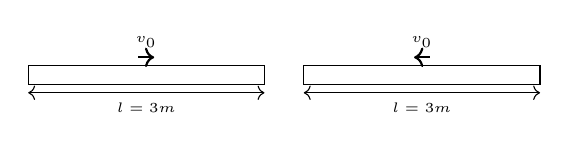
\begin{tikzpicture}
      \draw (0,0) rectangle (3,0.25);
      \draw[<->] (0,-0.1) -- (3,-0.1) node [midway, below] {\tiny $l=3m$};
      \draw[->,thick] (1.4,0.35) -- (1.6,0.35) node [midway, above] {\tiny $v_0$};
      \draw[<->] (3.5,-0.1) -- (6.5,-0.1) node [midway, below] {\tiny $l=3m$};
      \draw[<-,thick] (4.9,0.35) -- (5.1,0.35) node [midway, above] {\tiny $v_0$};
      \draw (3.5,0) rectangle (6.5,0.25);
    \end{tikzpicture}
  \end{block}
  \centering
  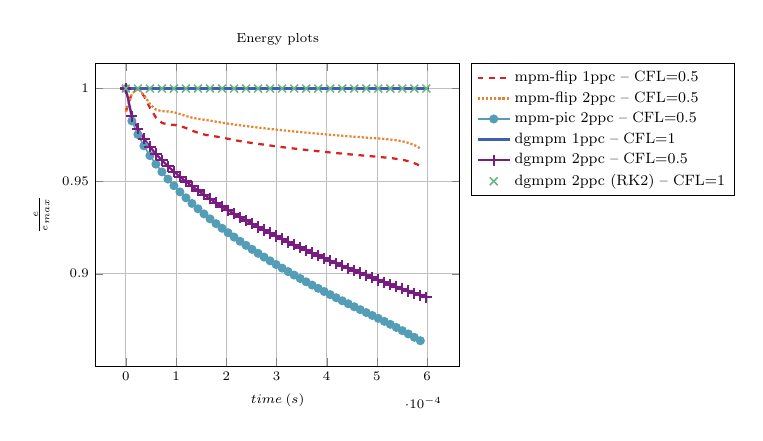
\begin{tikzpicture}[scale=.675]
\begin{axis}[xlabel=$time \: (s)$,ylabel=$\frac{e}{e_{max}}$,ymajorgrids=true,xmajorgrids=true,legend pos=outer north east,title={Energy plots}]
\addplot[Red,very thick,mark=none,dashed,mark size=2pt] coordinates {(0.0,0.987654320988) (1.2090867954e-05,0.997530864198) (2.41817359079e-05,1.0) (3.62726038619e-05,0.995910493827) (4.83634718158e-05,0.98940007716) (6.04543397698e-05,0.984093484761) (7.25452077237e-05,0.981362538279) (8.46360756777e-05,0.980572573344) (9.67269436317e-05,0.980353499636) (0.000108817811586,0.979737335844) (0.00012090867954,0.97855223305) (0.000132999547494,0.977156270039) (0.000145090415447,0.975958347691) (0.000157181283401,0.97511659562) (0.000169272151355,0.974530084065) (0.000181363019309,0.974005554053) (0.000193453887263,0.97341779498) (0.000205544755217,0.972760977912) (0.000217635623171,0.972101158286) (0.000229726491125,0.971500815494) (0.000241817359079,0.970976328432) (0.000253908227033,0.970503354023) (0.000265999094987,0.970047511625) (0.000278089962941,0.969589945626) (0.000290180830895,0.969132703566) (0.000302271698849,0.968688192138) (0.000314362566803,0.96826592316) (0.000326453434757,0.967866441189) (0.000338544302711,0.96748370195) (0.000350635170665,0.967111035083) (0.000362726038619,0.96674530374) (0.000374816906573,0.9663871534) (0.000386907774527,0.96603867283) (0.000398998642481,0.965701020803) (0.000411089510435,0.9653736209) (0.000423180378389,0.965054863002) (0.000435271246342,0.96474325827) (0.000447362114296,0.964438078134) (0.00045945298225,0.964139187671) (0.000471543850204,0.963846345834) (0.000483634718158,0.963558300848) (0.000495725586112,0.963271635613) (0.000507816454066,0.962978858237) (0.00051990732202,0.962665035247) (0.000531998189974,0.962302555824) (0.000544089057928,0.961844496637) (0.000556179925882,0.961218491107) (0.000568270793836,0.960324692645) (0.00058036166179,0.959042628999) (0.000592452529744,0.95725134199) };
\addplot[Orange,very thick,mark=none,densely dotted,mark size=3pt] coordinates {(0.0,0.987349583462) (1.19687379746e-05,0.997223079297) (2.39374759493e-05,1.0) (3.59062139239e-05,0.996543312249) (4.78749518985e-05,0.991672401699) (5.98436898731e-05,0.988645826067) (7.18124278478e-05,0.98773805255) (8.37811658224e-05,0.987631618227) (9.5749903797e-05,0.987207209533) (0.000107718641772,0.98625862112) (0.000119687379746,0.985162495947) (0.000131656117721,0.984278008796) (0.000143624855696,0.983664883566) (0.00015559359367,0.983176360212) (0.000167562331645,0.982669899583) (0.000179531069619,0.982113551237) (0.000191499807594,0.981554758898) (0.000203468545569,0.981041934115) (0.000215437283543,0.980583060318) (0.000227406021518,0.98015640132) (0.000239374759493,0.979740132791) (0.000251343497467,0.97932838866) (0.000263312235442,0.978927266369) (0.000275280973416,0.978543296202) (0.000287249711391,0.978177057907) (0.000299218449366,0.977824634311) (0.00031118718734,0.977482093196) (0.000323155925315,0.977147995987) (0.00033512466329,0.976822820567) (0.000347093401264,0.976507170495) (0.000359062139239,0.976200756538) (0.000371030877213,0.975902607469) (0.000382999615188,0.97561177268) (0.000394968353163,0.97532772239) (0.000406937091137,0.975050257459) (0.000418905829112,0.974779220922) (0.000430874567087,0.97451432881) (0.000442843305061,0.974255192075) (0.000454812043036,0.974001394871) (0.00046678078101,0.973752448152) (0.000478749518985,0.973507455428) (0.00049071825696,0.973264255861) (0.000502686994934,0.973017591891) (0.000514655732909,0.972755592972) (0.000526624470884,0.972453855054) (0.000538593208858,0.972067038786) (0.000550561946833,0.971519585751) (0.000562530684807,0.970699836135) (0.000574499422782,0.969464605892) (0.000586468160757,0.967662115176) };
\addplot[Duck,thick,mark=*,solid,mark size=2pt] coordinates {(0.0,1.0) (1.19687379746e-05,0.9825) (2.39374759493e-05,0.97517578125) (3.59062139239e-05,0.969031906128) (4.78749518985e-05,0.96380058825) (5.98436898731e-05,0.959171754479) (7.18124278478e-05,0.954982516842) (8.37811658224e-05,0.951129379832) (9.5749903797e-05,0.947543340455) (0.000107718641772,0.944175962079) (0.000119687379746,0.940991760326) (0.000131656117721,0.93796387047) (0.000143624855696,0.935071387013) (0.00015559359367,0.932297671085) (0.000167562331645,0.929629226561) (0.000179531069619,0.927054929147) (0.000191499807594,0.924565482142) (0.000203468545569,0.922153022591) (0.000215437283543,0.91981083008) (0.000227406021518,0.917533107309) (0.000239374759493,0.91531481198) (0.000251343497467,0.913151526055) (0.000263312235442,0.911039352738) (0.000275280973416,0.908974834313) (0.000287249711391,0.906954885898) (0.000299218449366,0.904976741526) (0.00031118718734,0.903037909836) (0.000323155925315,0.901136137378) (0.00033512466329,0.89926937799) (0.000347093401264,0.897435767059) (0.000359062139239,0.895633599746) (0.000371030877213,0.893861312443) (0.000382999615188,0.892117466744) (0.000394968353163,0.890400734736) (0.000406937091137,0.888709882017) (0.000418905829112,0.88704373739) (0.000430874567087,0.88540112132) (0.000442843305061,0.883780678009) (0.000454812043036,0.882180531538) (0.00046678078101,0.880597698856) (0.000478749518985,0.879027284148) (0.00049071825696,0.877461660668) (0.000502686994934,0.875890051367) (0.000514655732909,0.874299006831) (0.000526624470884,0.87267411056) (0.000538593208858,0.871002801233) (0.000550561946833,0.869277656037) (0.000562530684807,0.867499110287) (0.000574499422782,0.865676626234) (0.000586468160757,0.86382779387) };
\addplot[Blue,very thick,mark=none,solid,mark size=3pt] coordinates {(0.0,1.0) (2.41817359079e-05,1.0) (4.83634718158e-05,1.0) (7.25452077237e-05,1.0) (9.67269436317e-05,1.0) (0.00012090867954,1.0) (0.000145090415447,1.0) (0.000169272151355,1.0) (0.000193453887263,1.0) (0.000217635623171,1.0) (0.000241817359079,1.0) (0.000265999094987,1.0) (0.000290180830895,1.0) (0.000314362566803,1.0) (0.000338544302711,1.0) (0.000362726038619,1.0) (0.000386907774527,1.0) (0.000411089510435,1.0) (0.000435271246342,1.0) (0.00045945298225,1.0) (0.000483634718158,1.0) (0.000507816454066,1.0) (0.000531998189974,1.0) (0.000556179925882,1.0) (0.00058036166179,1.0) (0.000604543397698,1.0) };
\addplot[Purple,very thick,mark=+,solid,mark size=3pt] coordinates {(0.0,1.0) (1.19687379746e-05,0.985) (2.39374759493e-05,0.97828125) (3.59062139239e-05,0.972868652344) (4.78749518985e-05,0.968517532349) (5.98436898731e-05,0.964676422477) (7.18124278478e-05,0.961224535313) (8.37811658224e-05,0.95805841396) (9.5749903797e-05,0.955117021818) (0.000107718641772,0.952358340029) (0.000119687379746,0.949751847063) (0.000131656117721,0.947274776455) (0.000143624855696,0.944909512757) (0.00015559359367,0.942642119513) (0.000167562331645,0.940461338934) (0.000179531069619,0.938357922299) (0.000191499807594,0.936324160701) (0.000203468545569,0.934353548006) (0.000215437283543,0.932440533241) (0.000227406021518,0.93058033492) (0.000239374759493,0.928768799379) (0.000251343497467,0.927002291004) (0.000263312235442,0.925277605976) (0.000275280973416,0.923591903662) (0.000287249711391,0.921942651418) (0.000299218449366,0.920327579747) (0.00031118718734,0.918744645509) (0.000323155925315,0.917192001508) (0.00033512466329,0.915667971129) (0.000347093401264,0.91417102706) (0.000359062139239,0.9126997733) (0.000371030877213,0.911252929874) (0.000382999615188,0.909829319753) (0.000394968353163,0.908427857623) (0.000406937091137,0.907047540169) (0.000418905829112,0.905687437658) (0.000430874567087,0.904346686589) (0.000442843305061,0.903024483275) (0.000454812043036,0.901720078186) (0.00046678078101,0.900432770981) (0.000478749518985,0.899161906097) (0.00049071825696,0.897906868838) (0.000502686994934,0.896667081898) (0.000514655732909,0.895442002248) (0.000526624470884,0.894231118352) (0.000538593208858,0.89303394767) (0.000550561946833,0.891850034402) (0.000562530684807,0.890678947462) (0.000574499422782,0.889520278638) (0.000586468160757,0.888373640933) (0.000598436898731,0.887238667044) };
\addplot[Green,thick,mark=x,only marks,mark size=3pt] coordinates {(0.0,1.0) (2.39374759493e-05,1.0) (4.78749518985e-05,1.0) (7.18124278478e-05,1.0) (9.5749903797e-05,1.0) (0.000119687379746,1.0) (0.000143624855696,1.0) (0.000167562331645,1.0) (0.000191499807594,1.0) (0.000215437283543,1.0) (0.000239374759493,1.0) (0.000263312235442,1.0) (0.000287249711391,1.0) (0.00031118718734,1.0) (0.00033512466329,1.0) (0.000359062139239,1.0) (0.000382999615188,1.0) (0.000406937091137,1.0) (0.000430874567087,1.0) (0.000454812043036,1.0) (0.000478749518985,1.0) (0.000502686994934,1.0) (0.000526624470884,1.0) (0.000550561946833,1.0) (0.000574499422782,1.0) (0.000598436898731,1.0) };
\legend{mpm-flip 1ppc -- CFL=0.5,mpm-flip 2ppc -- CFL=0.5,mpm-pic 2ppc -- CFL=0.5,dgmpm 1ppc -- CFL=1,dgmpm 2ppc -- CFL=0.5,dgmpm 2ppc (RK2) -- CFL=1}
\end{axis}
\end{tikzpicture}
%%% Local Variables:
%%% mode: latex
%%% TeX-master: "../../presentation"
%%% End:

  \footnoteCite{Wang}
\end{frame}

\begin{frame}
  \begin{block}{Compression load on a one-dimensional Saint-Venant-Kirchhoff medium \cite{DGMPM}}
    \centering
    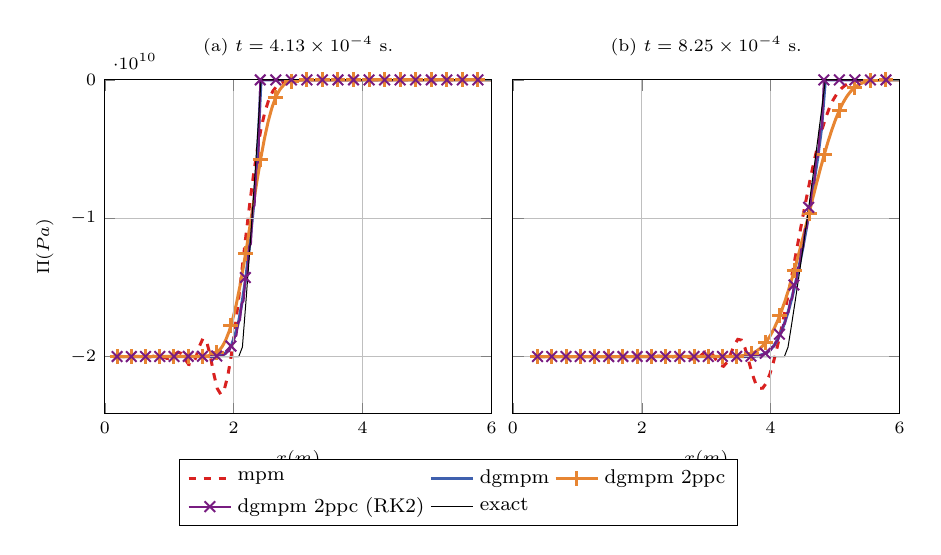
\begin{tikzpicture}[spy using outlines={rectangle, magnification=3, size=1.5cm, connect spies},scale=.9]
\begin{groupplot}[group style={group size=2 by 1,
ylabels at=edge left, yticklabels at=edge left,horizontal sep=2.ex,
vertical sep=4ex,xticklabels at=edge bottom,xlabels at=edge bottom},
ymajorgrids=true,xmajorgrids=true,enlargelimits=0,xmin=0.,xmax=6.,xlabel=$x (m)$,
axis on top,scale only axis,width=0.45\linewidth
]
\nextgroupplot[title={(a) $t = 4.13\times 10^{-4} $ s.},ymin=-24110446349.27083,ymax=0.0011926357337607983,ylabel=$\Pi (Pa)$,ymin=-24110446349.27083,ymax=0.0011926357337607983,]
\addplot[Red,dashed,mark=none,very thick,mark size=3pt,mark repeat=8] coordinates{(0.19074856210424165,-20008438887.20925) (0.24621817081166159,-19989354379.23872) (0.30168821376046606,-20005520602.82106) (0.35715707206163855,-19997317644.493065) (0.4126254059591947,-20009044796.22592) (0.4680939817653665,-19995691613.532185) (0.5235659892324547,-19985978703.12409) (0.5790381416586059,-19994717223.32923) (0.6345058419346248,-20015902240.556496) (0.6899678713027889,-20032823489.697666) (0.7454341765749165,-19987163582.169594) (0.8009140177508626,-19941824695.506912) (0.8564003699211709,-19943374447.68766) (0.9118703808647086,-20051664584.772846) (0.9673110818919248,-20140226838.362637) (1.0227456643110993,-20092736376.43716) (1.0782197499348205,-19874751801.04974) (1.1337532596053443,-19692570912.415062) (1.1893012287588407,-19777264946.626537) (1.2447784890024214,-20168408183.918118) (1.3001370554832676,-20572528821.830044) (1.355430995095431,-20599798630.13526) (1.4107977892703636,-20085736812.530434) (1.466361631166727,-19273984569.769203) (1.5221285414256531,-18706317605.373306) (1.577952808793877,-18882177214.574814) (1.6336065472853152,-19866938772.03486) (1.688913282617557,-21212062029.147175) (1.7438510744085634,-22297991777.82986) (1.7985557131985448,-22723359614.017532) (1.8532452770422718,-22395013283.985435) (1.9081388050549217,-21403637062.87418) (1.9634122329901567,-19894679452.103687) (2.0191884838071332,-18007718046.637062) (2.0755431379060907,-15864118384.038822) (2.1325129249654733,-13573203414.534416) (2.19010239286161,-11240530608.32656) (2.248288513254854,-8971445110.69128) (2.3070245345191696,-6867597798.321912) (2.366244538983924,-5017020633.538826) (2.425869591848499,-3481241892.4944673) (2.485815404623328,-2285084685.027758) (2.54600044341317,-1414457405.5589426) (2.6063528607822968,-823946038.6228448) (2.6668148407035575,-451202528.72253466) (2.7273438166817074,-232224243.4824339) (2.7879110500643134,-112369125.93567534) (2.848498696235943,-51151029.04724893) (2.90909653054647,-21919180.7929816) (2.969699127892279,-8847440.992686674) (3.030303813846766,-3365310.2671077778) (3.090909359861519,-1206564.3711837244) (3.1515152387675816,-407761.1863610826) (3.212121238860824,-129870.91020548563) (3.272727280463445,-38967.23655715507) (3.3333333354445758,-11008.093626811817) (3.39393939448235,-2925.529133049118) (3.454545454676886,-730.7044499386213) (3.515151515181421,-171.3150988590629) (3.5757575757639617,-37.64768411548184) (3.636363636364914,-7.741640661862447) (3.6969696969699357,-1.4866996522755471) (3.7575757575758,-0.26599662643451877) (3.818181818181825,-0.044238117442756235) (3.87878787878788,-0.006815061335775961) (3.9393939393939394,-0.000956499836600135) (4.0,-0.00011956247957501687) (4.0606060606060606,0.0) (4.121212121212121,0.0) (4.181818181818182,0.0) (4.242424242424242,0.0) (4.303030303030303,0.0) (4.363636363636363,0.0) (4.424242424242425,0.0) (4.484848484848485,0.0) (4.545454545454546,0.0) (4.606060606060606,0.0) (4.666666666666667,0.0) (4.7272727272727275,0.0) (4.787878787878788,0.0) (4.848484848484849,0.0) (4.909090909090909,0.0) (4.96969696969697,0.0) (5.03030303030303,0.0) (5.090909090909091,0.0) (5.151515151515151,0.0) (5.212121212121212,0.0) (5.2727272727272725,0.0) (5.333333333333334,0.0) (5.3939393939393945,0.0) (5.454545454545455,0.0) (5.515151515151516,0.0) (5.575757575757576,0.0) (5.636363636363637,0.0) (5.696969696969697,0.0) (5.757575757575758,0.0) (5.818181818181818,0.0) (5.878787878787879,0.0) (5.9393939393939394,0.0) (6.0,0.0) };
\addplot[Blue,solid,mark=none,very thick,mark size=3pt,mark repeat=8] coordinates{(0.19184481823272587,-20000746788.895386) (0.2472984593148165,-19999262845.167934) (0.3027550579515747,-20000799959.541138) (0.3582139828028267,-19999230865.055157) (0.4136744334611789,-20000901266.778095) (0.4691363798583578,-19999156573.758553) (0.5245991019399393,-20001058323.113438) (0.5800629488714097,-19999036648.84517) (0.635527105553384,-20001282242.769444) (0.6909922402572966,-19998864927.72781) (0.7464573416593343,-20001588390.21625) (0.8019234043904636,-19998632043.305565) (0.8573891369717147,-20001997440.71843) (0.9128559063396893,-19998324890.49686) (0.9683220513996212,-20002536843.16476) (1.023789388354951,-19997925908.97679) (1.0792557790732065,-20003242807.18485) (1.1347235977259633,-19997412156.041016) (1.1901900940405064,-20004162964.68389) (1.2456583458259118,-19996754091.63044) (1.3011248178858221,-20005359727.42986) (1.3565934830124184,-19995913073.930134) (1.412059799077113,-20006909700.64143) (1.467528884562971,-19994813482.07538) (1.5229949116205286,-20008792500.146915) (1.5784645009572125,-19992861846.161507) (1.63393029649414,-20009157097.143948) (1.689401269313731,-19983335218.807507) (1.7448693336716496,-19988556060.043617) (1.8003496405947086,-19915211430.44971) (1.8558399943620645,-19832464370.455975) (1.9113756485372175,-19565996896.830357) (1.9669788598771232,-19175060421.84385) (2.022726722440876,-18428718648.265965) (2.078678157853173,-17432821776.53043) (2.134949207911814,-15950492705.79851) (2.191612836208383,-14179637125.40624) (2.248793446466984,-11863860055.04507) (2.3065513731895595,-9241855726.717867) (2.365009406439806,-5893766492.953189) (2.4242424242424243,0.0) (2.484848484848485,0.0) (2.5454545454545454,0.0) (2.606060606060606,0.0) (2.666666666666667,0.0) (2.7272727272727275,0.0) (2.787878787878788,0.0) (2.8484848484848486,0.0) (2.909090909090909,0.0) (2.9696969696969697,0.0) (3.0303030303030303,0.0) (3.090909090909091,0.0) (3.1515151515151514,0.0) (3.2121212121212124,0.0) (3.272727272727273,0.0) (3.3333333333333335,0.0) (3.393939393939394,0.0) (3.4545454545454546,0.0) (3.515151515151515,0.0) (3.5757575757575757,0.0) (3.6363636363636367,0.0) (3.6969696969696972,0.0) (3.757575757575758,0.0) (3.8181818181818183,0.0) (3.878787878787879,0.0) (3.9393939393939394,0.0) (4.0,0.0) (4.0606060606060606,0.0) (4.121212121212121,0.0) (4.181818181818182,0.0) (4.242424242424242,0.0) (4.303030303030303,0.0) (4.363636363636363,0.0) (4.424242424242425,0.0) (4.484848484848485,0.0) (4.545454545454546,0.0) (4.606060606060606,0.0) (4.666666666666667,0.0) (4.7272727272727275,0.0) (4.787878787878788,0.0) (4.848484848484849,0.0) (4.909090909090909,0.0) (4.96969696969697,0.0) (5.03030303030303,0.0) (5.090909090909091,0.0) (5.151515151515151,0.0) (5.212121212121212,0.0) (5.2727272727272725,0.0) (5.333333333333334,0.0) (5.3939393939393945,0.0) (5.454545454545455,0.0) (5.515151515151516,0.0) (5.575757575757576,0.0) (5.636363636363637,0.0) (5.696969696969697,0.0) (5.757575757575758,0.0) (5.818181818181818,0.0) (5.878787878787879,0.0) (5.9393939393939394,0.0) (6.0,0.0) };
\addplot[Orange,solid,mark=+,very thick,mark size=3pt,mark repeat=8] coordinates{(0.18995525166111366,-19999912858.22518) (0.21763857805956868,-19999769787.88829) (0.24512208706281055,-19999595225.830395) (0.27282575705740886,-19999451694.173355) (0.3003071750929951,-19999276292.69227) (0.32801595744355366,-19999131832.277004) (0.3554953427946694,-19998955018.611973) (0.3832066011773739,-19998809148.97717) (0.4106846406234849,-19998630330.553932) (0.4383974367587157,-19998482551.158222) (0.46587453401796425,-19998301106.73408) (0.49358840901570517,-19998150889.20853) (0.5210648104045611,-19997966159.024174) (0.5487795002679247,-19997812938.436954) (0.5762553672290964,-19997624212.983093) (0.6039707041588833,-19997467377.749435) (0.6314461490108538,-19997273884.659058) (0.659162018895618,-19997112764.632294) (0.6866371235984735,-19996913653.070396) (0.7143534449920753,-19996747505.207943) (0.7418282717305508,-19996541826.930435) (0.7695449843941599,-19996369817.725258) (0.7970195819297244,-19996156503.688694) (0.8247366401192712,-19995977687.259945) (0.8522110478099802,-19995755518.23956) (0.8799284161209588,-19995568808.532024) (0.9074026665852393,-19995336377.560326) (0.9351203172698606,-19995140512.397816) (0.9625944382274981,-19994896175.737343) (0.9903123494081251,-19994689669.049244) (1.0177863650063577,-19994431479.734898) (1.0455045194632855,-19994212553.503006) (1.0729784512767135,-19993938160.470367) (1.1006968356268219,-19993704624.606678) (1.1281707034621382,-19993411064.120533) (1.1558893076415115,-19993159994.96435) (1.1833631302893026,-19992843029.618053) (1.2110819473987793,-19992569575.424583) (1.2385557436795793,-19992221110.35909) (1.2662747707021536,-19991913792.57851) (1.2937485620273468,-19991511992.659107) (1.3214678034398997,-19991135778.789246) (1.348941622020031,-19990611361.07096) (1.3766611027821543,-19990054404.717606) (1.4041350176396072,-19989191087.10363) (1.43185482298986,-19988120795.17056) (1.4593290140068589,-19986303943.14754) (1.4870493950945292,-19983836663.36228) (1.5145243372708168,-19979517453.333805) (1.5422459535049426,-19973584795.21019) (1.5697228130621068,-19963335295.939476) (1.5974472092249048,-19949696944.16045) (1.6249285708236694,-19926887514.67977) (1.6526589729400751,-19897960308.693275) (1.6801499595587883,-19851437924.117283) (1.7078923745712826,-19795437569.700573) (1.7354020457070085,-19708969482.813923) (1.7631664627875865,-19610053565.1548) (1.7907091203275556,-19463351503.24422) (1.8185104215571681,-19303209212.943596) (1.846106271632855,-19074774470.23491) (1.8739644155740336,-18835426807.336002) (1.9016391139595983,-18506490966.59541) (1.929578344685977,-18173408100.377052) (1.9573613220878685,-17731609002.064552) (1.9854084938213,-17296152224.080425) (2.013330410494915,-16737796934.560286) (2.041512798178765,-16198491879.856827) (2.069602736105936,-15529090279.041159) (2.097945774544229,-14891880186.885708) (2.1262287257995864,-14125409710.52269) (2.154753998432247,-13403375220.585518) (2.1832489573267595,-12561011287.379313) (2.211972566392059,-11773975414.023428) (2.24069126999827,-10882817742.279064) (2.2696225838776267,-10056933247.623539) (2.2985687962945347,-9148834985.540192) (2.327709541119762,-8315860661.742456) (2.356878766471977,-7426050359.213425) (2.3862225001407333,-6621710808.248219) (2.4156021007706037,-5786632187.628343) (2.4451342315442015,-5047407133.728801) (2.47470405839892,-4301249043.455953) (2.5044026660566034,-3659402379.111651) (2.5341363952031912,-3029346440.874573) (2.563974070845136,-2507081699.0016084) (2.593841384344465,-2008351349.8441858) (2.623788042880702,-1613201600.0153964) (2.6537575319704074,-1245972269.7087686) (2.6837837243855356,-969806805.9692637) (2.713826006898169,-719895044.9301026) (2.743905915736818,-542465644.1033932) (2.773996200748826,-386006963.2538726) (2.804109532245024,-281510641.82021976) (2.8342289849581657,-191643401.31466892) (2.8643614213299275,-135290962.20125788) (2.8944971613083075,-87983443.40475516) (2.924639617951817,-60153986.76079956) (2.9547837066305997,-37328498.31375421) (2.9849309849010037,-24733077.95371384) (3.015079001851262,-14631759.500679849) (3.045228409801474,-9402072.941124339) (3.0753781243862,-5298061.620119785) (3.105528396475034,-3304104.722537816) (3.1356787854200334,-1771954.9486091677) (3.1658293798711896,-1073279.4290237231) (3.195980015238912,-547296.2783473512) (3.226130720321594,-322187.11395850533) (3.2562814385751238,-156061.14816243792) (3.286432178602333,-89350.21257776454) (3.316582922528392,-41065.456399169176) (3.3467336727166184,-22880.71737255304) (3.3768844239662927,-9965.667379406394) (3.4070351768743565,-5407.004064866737) (3.437185930048142,-2228.6748053008914) (3.4673366836262214,-1178.1706413573809) (3.497487437265445,-458.856763768479) (3.527638190995354,-236.47913094118658) (3.5577889447381867,-86.87293189700003) (3.587939698499721,-43.6702853295511) (3.618090452263762,-15.102474825431294) (3.6482412060313454,-7.4089580622410764) (3.6783919597993746,-2.406673151344001) (3.7085427135680193,-1.1526420843380152) (3.7386934673367365,-0.35061697135328035) (3.768844221105552,-0.1639201594972483) (3.798994974874379,-0.04639024207509855) (3.8291457286432187,-0.02113266826488257) (3.8592964824120606,-0.005410202200769404) (3.8894472361809047,-0.002271687111925301) (3.9195979899497484,-0.00044835929840631247) (3.949748743718593,-0.00017934371936252516) (3.979899497487437,0.0) (4.010050251256281,0.0) (4.040201005025126,0.0) (4.0703517587939695,0.0) (4.100502512562814,0.0) (4.130653266331658,-5.9781239787508415e-05) (4.160804020100502,0.0) (4.190954773869347,0.0) (4.221105527638191,0.0) (4.251256281407035,0.0) (4.281407035175879,0.0) (4.311557788944723,0.0) (4.341708542713568,0.0) (4.371859296482412,0.0) (4.402010050251256,0.0) (4.4321608040201,-5.9781239787508415e-05) (4.4623115577889445,0.0) (4.492462311557789,0.0) (4.522613065326633,0.0) (4.552763819095477,0.0) (4.582914572864321,0.0) (4.613065326633166,0.0) (4.64321608040201,0.0) (4.673366834170854,0.0) (4.703517587939698,0.0) (4.733668341708542,0.0) (4.763819095477387,0.0) (4.793969849246231,0.0) (4.824120603015075,0.0) (4.8542713567839195,0.0) (4.884422110552763,0.0) (4.914572864321608,0.0) (4.944723618090452,0.0) (4.974874371859296,0.0) (5.005025125628141,0.0) (5.035175879396984,0.0) (5.065326633165829,0.0) (5.0954773869346734,0.0) (5.125628140703517,0.0) (5.155778894472362,0.0) (5.185929648241205,0.0) (5.21608040201005,0.0) (5.2462311557788945,0.0) (5.276381909547738,-5.9781239787508415e-05) (5.306532663316583,0.0) (5.3366834170854265,0.0) (5.366834170854271,0.0) (5.396984924623116,0.0) (5.427135678391959,0.0) (5.457286432160804,0.0) (5.487437185929648,0.0) (5.517587939698492,0.0) (5.547738693467337,0.0) (5.57788944723618,0.0) (5.608040201005025,0.0) (5.638190954773869,-5.9781239787508415e-05) (5.668341708542713,0.0) (5.698492462311558,0.0) (5.7286432160804015,0.0) (5.758793969849246,0.0) (5.788944723618091,0.0) (5.819095477386934,0.0) (5.849246231155779,0.0) (5.879396984924623,-5.9781239787508415e-05) (5.909547738693467,0.0) (5.939698492462312,0.0) (5.969849246231155,0.0) (6.0,0.0) };
\addplot[Purple,solid,mark=x,thick,mark size=3pt,mark repeat=8] coordinates{(0.19087078866902665,-19999455640.176197) (0.22071218292775385,-19999409659.864017) (0.2459924077656396,-20000077312.85232) (0.27597326522813487,-20000072009.997063) (0.3011894927456019,-19998950742.164944) (0.3311766255539742,-19998862763.515118) (0.3563962430072859,-19999589159.90041) (0.38636963567121163,-19999626165.686943) (0.41160234396465,-19998404877.00223) (0.4415609586628959,-19998270520.060898) (0.4668064289385858,-19999118873.727676) (0.49675180124731944,-19999202922.963924) (0.5220088990140508,-19997806766.43407) (0.5519428363462726,-19997618279.35031) (0.5772098159593475,-19998661098.62433) (0.6071336614902496,-19998800403.628937) (0.6324097933704171,-19997141589.490086) (0.6623248466555562,-19996887265.347076) (0.6876086367678674,-19998211885.709827) (0.7175157537096876,-19998418772.38764) (0.7428070060201625,-19996389972.392735) (0.7727071471896477,-19996053259.198273) (0.7980044513100885,-19997768502.897907) (0.8278981543338224,-19998060358.486023) (0.8532017639590902,-19995526549.26538) (0.8830898001721301,-19995084778.141758) (0.9083982334111295,-19997329243.71315) (0.9382809151671918,-19997729846.142517) (0.9635948605946703,-19994517924.97995) (0.9934728615949118,-19993940550.927967) (1.018790634157661,-19996893154.38264) (1.0486640867664065,-19997434481.72408) (1.0739868482392012,-19993319799.35868) (1.103856391967528,-19992566008.07375) (1.129182120960812,-19996459571.531334) (1.1590477257284901,-19997184225.495197) (1.1843781409943626,-19991872941.060112) (1.2142404634066721,-19990888423.449177) (1.2395730548989103,-19996027394.59501) (1.269431901039365,-19996991817.22908) (1.2947690752904193,-19990097771.00673) (1.3246251669949154,-19988810395.611206) (1.3499637385624637,-19995594394.611435) (1.3798167010879285,-19996873032.549503) (1.4051599499623135,-19987887684.922043) (1.4350106214725087,-19986201196.541973) (1.4603544495160277,-19995154760.05428) (1.4902022422851016,-19996842075.848194) (1.5155510581278278,-19985077422.35594) (1.5453969866641184,-19982845663.359066) (1.570745480163516,-19994550689.773247) (1.6005886999258214,-19996684108.793686) (1.625942792905406,-19980692933.116657) (1.6557845912583171,-19977385747.898075) (1.6811375441326768,-19990452521.34305) (1.7109768445952687,-19991936790.38711) (1.736337222388458,-19962562834.670414) (1.7661759691627483,-19954268934.61151) (1.7915371396346151,-19946636578.575214) (1.8213747099598598,-19938461812.41097) (1.8467537764093123,-19837157162.8332) (1.8765945013072705,-19804712010.78011) (1.9019952765295465,-19662159771.99236) (1.9318415620560758,-19612768170.569878) (1.9573086438181697,-19243797603.252537) (1.987170301328827,-19145197075.79308) (2.012739158284794,-18606422582.842396) (2.042623150182732,-18474857956.820774) (2.068383513683698,-17546640829.370663) (2.0983030697861436,-17356604515.480618) (2.1243218125728434,-16168446386.224903) (2.154282226835199,-15957833195.666677) (2.1806765607592036,-14287253493.297613) (2.2106861953891266,-14032581607.352451) (2.2375256180290903,-12078287603.813477) (2.2675794640427664,-11846950370.664488) (2.2949840954789456,-9331938813.91532) (2.325083226953284,-9055544632.420107) (2.3531208903662257,-6074271277.8443) (2.3832414203422285,-5944142832.467713) (2.4120603015075375,0.0004184686785125597) (2.4422110552763816,0.0004184686785125597) (2.472361809045226,0.000717374877450103) (2.5025125628140703,0.000717374877450103) (2.5326633165829144,0.0001793437193625254) (2.5628140703517586,0.0001793437193625254) (2.5929648241206027,0.0005978123978750856) (2.6231155778894473,0.0005978123978750856) (2.6532663316582914,0.0005978123978750856) (2.6834170854271355,0.0005978123978750856) (2.7135678391959797,0.0006575936376625943) (2.743718592964824,0.0005978123978750856) (2.7738693467336684,0.0005380311580875769) (2.8040201005025125,0.0004782499183000683) (2.8341708542713566,0.0003586874387250511) (2.8643216080402008,0.0003586874387250511) (2.8944723618090453,0.00011956247957501691) (2.9246231155778895,0.00011956247957501691) (2.9547738693467336,0.0005380311580875769) (2.9849246231155777,0.0004782499183000683) (3.015075376884422,0.0005380311580875769) (3.0452261306532664,0.0005380311580875769) (3.0753768844221105,0.000717374877450103) (3.1055276381909547,0.000717374877450103) (3.135678391959799,0.0001793437193625254) (3.165829145728643,0.00011956247957501691) (3.1959798994974875,0.0005978123978750856) (3.2261306532663316,0.0005978123978750856) (3.2562814070351758,0.0004782499183000683) (3.28643216080402,0.0004782499183000683) (3.316582914572864,0.0002989061989375425) (3.3467336683417086,0.00023912495915003393) (3.3768844221105527,0.0005978123978750856) (3.407035175879397,0.0005380311580875769) (3.437185929648241,0.0004184686785125597) (3.467336683417085,0.0004184686785125597) (3.4974874371859297,0.0002989061989375425) (3.527638190954774,0.0002989061989375425) (3.557788944723618,5.978123978750844e-05) (3.587939698492462,5.978123978750844e-05) (3.618090452261306,0.00011956247957501691) (3.648241206030151,0.0) (3.678391959798995,0.0001793437193625254) (3.708542713567839,0.00011956247957501691) (3.738693467336683,0.0005978123978750856) (3.7688442211055273,0.0005978123978750856) (3.798994974874372,0.0) (3.829145728643216,-0.0001195624795750168) (3.85929648241206,0.0003586874387250511) (3.8894472361809043,0.0002989061989375425) (3.9195979899497484,0.0004782499183000683) (3.949748743718593,0.0004782499183000683) (3.979899497487437,0.00011956247957501691) (4.010050251256281,5.978123978750844e-05) (4.040201005025126,-0.00032879681883129597) (4.0703517587939695,-0.00032879681883129597) (4.100502512562814,0.0005978123978750856) (4.130653266331658,0.0005978123978750856) (4.160804020100502,0.0) (4.190954773869347,0.00011956247957501691) (4.221105527638191,0.0005978123978750856) (4.251256281407035,0.0005978123978750856) (4.281407035175879,0.00023912495915003393) (4.311557788944723,0.00023912495915003393) (4.341708542713568,-5.9781239787508415e-05) (4.371859296482412,-0.0001195624795750168) (4.402010050251256,0.0005978123978750856) (4.4321608040201,0.0005978123978750856) (4.4623115577889445,-0.00044835929840631247) (4.492462311557789,-0.00044835929840631247) (4.522613065326633,0.0004782499183000683) (4.552763819095477,0.0005380311580875769) (4.582914572864321,0.0001793437193625254) (4.613065326633166,0.00011956247957501691) (4.64321608040201,0.0005978123978750856) (4.673366834170854,0.0005380311580875769) (4.703517587939698,0.0006575936376625943) (4.733668341708542,0.0006575936376625943) (4.763819095477387,-0.00032879681883129597) (4.793969849246231,-0.00032879681883129597) (4.824120603015075,0.0005978123978750856) (4.8542713567839195,0.0005978123978750856) (4.884422110552763,-0.00029890619893754183) (4.914572864321608,-0.00029890619893754183) (4.944723618090452,0.0006575936376625943) (4.974874371859296,0.0005978123978750856) (5.005025125628141,-0.00032879681883129597) (5.035175879396984,-0.00032879681883129597) (5.065326633165829,0.00023912495915003393) (5.0954773869346734,0.00023912495915003393) (5.125628140703517,0.0003586874387250511) (5.155778894472362,0.0004184686785125597) (5.185929648241205,-0.00044835929840631247) (5.21608040201005,-0.00032879681883129597) (5.2462311557788945,0.0005978123978750856) (5.276381909547738,0.0005978123978750856) (5.306532663316583,0.00023912495915003393) (5.3366834170854265,0.00023912495915003393) (5.366834170854271,-0.00044835929840631247) (5.396984924623116,-0.0003885780586188042) (5.427135678391959,0.0003586874387250511) (5.457286432160804,0.0004184686785125597) (5.487437185929648,-0.0003885780586188042) (5.517587939698492,-0.00044835929840631247) (5.547738693467337,0.0005978123978750856) (5.57788944723618,0.0005978123978750856) (5.608040201005025,-0.00029890619893754183) (5.638190954773869,-0.00029890619893754183) (5.668341708542713,0.0006575936376625943) (5.698492462311558,0.0006575936376625943) (5.7286432160804015,-0.00017934371936252516) (5.758793969849246,-0.00017934371936252516) (5.788944723618091,-0.00032879681883129597) (5.819095477386934,-0.00032879681883129597) (5.849246231155779,0.0006575936376625943) (5.879396984924623,0.0006575936376625943) (5.909547738693467,-0.00032879681883129597) (5.939698492462312,-0.00032879681883129597) (5.969849246231155,0.0011358435559626649) (6.0,0.0007771561172376117) };
\addplot[black,solid,mark=none,thin,mark size=3pt,mark repeat=8] coordinates{(0.19184481823272587,-19999999999.99513) (0.2472984593148165,-19999999999.99513) (0.3027550579515747,-19999999999.99513) (0.3582139828028267,-19999999999.99513) (0.4136744334611789,-19999999999.99513) (0.4691363798583578,-19999999999.99513) (0.5245991019399393,-19999999999.99513) (0.5800629488714097,-19999999999.99513) (0.635527105553384,-19999999999.99513) (0.6909922402572966,-19999999999.99513) (0.7464573416593343,-19999999999.99513) (0.8019234043904636,-19999999999.99513) (0.8573891369717147,-19999999999.99513) (0.9128559063396893,-19999999999.99513) (0.9683220513996212,-19999999999.99513) (1.023789388354951,-19999999999.99513) (1.0792557790732065,-19999999999.99513) (1.1347235977259633,-19999999999.99513) (1.1901900940405064,-19999999999.99513) (1.2456583458259118,-19999999999.99513) (1.3011248178858221,-19999999999.99513) (1.3565934830124184,-19999999999.99513) (1.412059799077113,-19999999999.99513) (1.467528884562971,-19999999999.99513) (1.5229949116205286,-19999999999.99513) (1.5784645009572125,-19999999999.99513) (1.63393029649414,-19999999999.99513) (1.689401269313731,-19999999999.99513) (1.7448693336716496,-19999999999.99513) (1.8003496405947086,-19999999999.99513) (1.8558399943620645,-19999999999.99513) (1.9113756485372175,-19999999999.99513) (1.9669788598771232,-19999999999.99513) (2.022726722440876,-19999999999.99513) (2.078678157853173,-19999999999.99513) (2.134949207911814,-19320644756.027233) (2.191612836208383,-15934816130.431961) (2.248793446466984,-12317415446.21064) (2.3065513731895595,-8460847327.543606) (2.365009406439806,-4357551166.693738) (2.4242424242424243,-8.967185968126261e-05) (2.484848484848485,0.0) (2.5454545454545454,0.0) (2.606060606060606,0.0) (2.666666666666667,0.0) (2.7272727272727275,0.0) (2.787878787878788,0.0) (2.8484848484848486,0.0) (2.909090909090909,0.0) (2.9696969696969697,0.0) (3.0303030303030303,0.0) (3.090909090909091,0.0) (3.1515151515151514,0.0) (3.2121212121212124,0.0) (3.272727272727273,0.0) (3.3333333333333335,0.0) (3.393939393939394,0.0) (3.4545454545454546,0.0) (3.515151515151515,0.0) (3.5757575757575757,0.0) (3.6363636363636367,0.0) (3.6969696969696972,0.0) (3.757575757575758,0.0) (3.8181818181818183,0.0) (3.878787878787879,0.0) (3.9393939393939394,0.0) (4.0,0.0) (4.0606060606060606,0.0) (4.121212121212121,0.0) (4.181818181818182,0.0) (4.242424242424242,0.0) (4.303030303030303,0.0) (4.363636363636363,0.0) (4.424242424242425,0.0) (4.484848484848485,0.0) (4.545454545454546,0.0) (4.606060606060606,0.0) (4.666666666666667,0.0) (4.7272727272727275,0.0) (4.787878787878788,0.0) (4.848484848484849,0.0) (4.909090909090909,0.0) (4.96969696969697,0.0) (5.03030303030303,0.0) (5.090909090909091,0.0) (5.151515151515151,0.0) (5.212121212121212,0.0) (5.2727272727272725,0.0) (5.333333333333334,0.0) (5.3939393939393945,0.0) (5.454545454545455,0.0) (5.515151515151516,0.0) (5.575757575757576,0.0) (5.636363636363637,0.0) (5.696969696969697,0.0) (5.757575757575758,0.0) (5.818181818181818,0.0) (5.878787878787879,0.0) (5.9393939393939394,0.0) (6.0,0.0) };
\nextgroupplot[title={(b) $t = 8.25\times 10^{-4} $ s.},ymin=-24110446349.27083,ymax=0.0011926357337607983,legend style={at={($(0.5,-0.35)+(0.45cm,1cm)$)},legend columns=3},ymin=-24110446349.27083,ymax=0.0011926357337607983]
\addplot[Red,dashed,mark=none,very thick,mark size=3pt,mark repeat=8] coordinates{(0.38293910383528906,-20003193601.32246) (0.43840837199947835,-19996890010.44354) (0.49387769714078006,-20002810664.06406) (0.5493469460436499,-19997402454.49987) (0.604816307544493,-20002053897.092567) (0.6602855453528985,-19998233855.330673) (0.7157549302044005,-20001065610.299152) (0.7712241771874568,-19999160525.93578) (0.8266935740052295,-20000058542.932457) (0.8821628347146323,-20000075351.33247) (0.9376322196789464,-19999223388.544975) (0.9931015144747715,-20000681392.727028) (1.0485709116090554,-19998535531.845932) (1.1040402473751902,-20001093857.236908) (1.159509599800273,-19998423559.75984) (1.2149789261281079,-20001269259.8173) (1.2704483032029954,-19998082465.22125) (1.3259177617113134,-20000721934.62686) (1.3813871777131423,-19998368171.224865) (1.4368565024667654,-20001335225.921165) (1.4923257124577392,-19999139537.473896) (1.5477951245250876,-19999977034.808746) (1.603264800420931,-19997366223.445232) (1.658734561549041,-19999404163.79598) (1.714203821740546,-20000733203.519554) (1.7696725521519512,-20002964876.199337) (1.8251414364045961,-19999699201.181786) (1.8806114999051913,-19995038708.093014) (1.9360825767965035,-19992887493.07817) (1.99155299294749,-19999479929.740265) (2.047020933029572,-20009529426.978573) (2.1024869963536044,-20012092799.86235) (2.157954653494298,-19998817774.306145) (2.21342730550197,-19978518214.160187) (2.2689038601486224,-19972580455.985214) (2.3243778325315083,-19995878228.36715) (2.3798424512126446,-20035444573.81262) (2.435298411182689,-20054049739.716343) (2.490756489519581,-20021213677.526375) (2.5462302699519013,-19948514392.93821) (2.601723075226865,-19893245484.628185) (2.6572204391174483,-19917838301.721115) (2.7126973065494653,-20031100173.360226) (2.7681376892592082,-20162884506.663513) (2.8235523095290347,-20203893116.997597) (2.8789781375297894,-20087722832.88711) (2.9344559643028174,-19854579711.64403) (2.989999209962102,-19646990335.081882) (3.045575896882743,-19628779834.71236) (3.1011196727533443,-19869145766.38885) (3.156567579543061,-20273690673.83133) (3.2119025585950145,-20624800683.39243) (3.2671727366500503,-20705420466.33008) (3.3224741150036348,-20417048868.592064) (3.3779059985229227,-19832497191.738167) (3.433521436268489,-19178965694.534603) (3.4892948375799326,-18757546044.958984) (3.545122418371894,-18808323074.271023) (3.6008593047641337,-19377191208.346) (3.6563784539570743,-20283488062.88574) (3.7116207922560704,-21227435472.844982) (3.766610481918908,-21947434680.918854) (3.821434331547984,-22306543493.006428) (3.8762062128294406,-22283379201.176712) (3.9310377197740727,-21921087856.23185) (3.9860230078363736,-21283036693.95003) (4.041235051381953,-20429288993.550903) (4.096727730149534,-19408706715.401764) (4.15253967486421,-18258789809.14372) (4.208697897594965,-17008231371.292692) (4.265220559254305,-15679915563.06747) (4.322118823472007,-14293588835.728102) (4.379397942897866,-12868046999.275988) (4.437057759764468,-11422841891.222075) (4.495092796347134,-9979483421.353954) (4.553492108773863,-8562028244.002579) (4.612239088346305,-7196883036.548134) (4.6713114078106015,-5911668571.452027) (4.73068130557479,-4733132590.811638) (4.790316357237068,-3684362130.566879) (4.850180789776346,-2781852608.3265805) (4.910237259771771,-2033195810.7329576) (4.970448878797953,-1436101822.5106232) (5.030781177054902,-979120915.605681) (5.091203691445661,-643898192.5793709) (5.151690954192834,-408317639.6226731) (5.212222808903811,-249692315.627806) (5.272784134359923,-147293016.37721288) (5.333364159779438,-83859339.43092377) (5.3939555862511845,-46108252.305678315) (5.454553698033615,-24498793.547717854) (5.515155583994159,-12587098.702215005) (5.575759523473027,-6257199.615622005) (5.636364540851207,-3011210.1817965256) (5.69697010455805,-1403486.7621329858) (5.757575935864655,-633737.4923960958) (5.818181893951029,-277107.8297423803) (5.878787910227981,-116738.74654983562) (5.939393952555769,-45656.59030542923) (6.0000000066884045,-11857.277843346354) };
\addplot[Blue,solid,mark=none,very thick,mark size=3pt,mark repeat=8] coordinates{(0.38401698079958846,-19999993425.18581) (0.4394706083791145,-19999974753.481766) (0.4949272641367282,-19999961717.61289) (0.5503861475694772,-19999942904.998543) (0.6058467157310151,-19999930217.40262) (0.6613085899995965,-19999911111.718575) (0.7167714966962511,-19999899028.369488) (0.7722352359338598,-19999879454.1201) (0.8276996549718213,-19999868268.3495) (0.8831646391924676,-19999848012.893536) (0.9386300959070943,-19999838073.78776) (0.9940959553211544,-19999816870.787548) (1.0495621569710856,-19999808605.328205) (1.105028656709029,-19999786114.244507) (1.160495412363306,-19999780054.698708) (1.2159623956589096,-19999755834.83223) (1.2714295751240139,-19999752653.273045) (1.3268969331110458,-19999726130.46261) (1.382364444349215,-19999726682.80252) (1.4378320989435756,-19999697106.363777) (1.4932998749050497,-19999702488.96461) (1.5487677685712533,-19999668875.7513) (1.6042357591292715,-19999680498.572514) (1.6597038484858433,-19999641560.122932) (1.7151720152881706,-19999661241.559338) (1.770640266961506,-19999615289.08321) (1.82610858002389,-19999645379.208828) (1.8815769678746177,-19999590199.591084) (1.937045403252577,-19999633740.59181) (1.9925139064694894,-19999566434.536407) (2.0479824446167614,-19999627369.833504) (2.103451046375716,-19999544140.596123) (2.1589196709486864,-19999627587.748276) (2.2143883574489496,-19999523465.442642) (2.269857054403287,-19999636072.65706) (2.325325814161538,-19999504554.63235) (2.380794571038499,-19999654966.98424) (2.4362633943617333,-19999487548.98547) (2.491732199691955,-19999687018.771164) (2.5472010782759194,-19999472584.149097) (2.6026699210461697,-19999735770.857525) (2.658138847661513,-19999459795.547363) (2.71360771679892,-19999805815.665028) (2.7690766850365396,-19999449334.413616) (2.824545568867529,-19999903140.84676) (2.8800145729191846,-19999441404.346233) (2.9354834585578145,-20000035600.77515) (2.990952493008963,-19999436331.18854) (3.046421365622187,-20000213553.42369) (3.1018904252350925,-19999434649.634323) (3.1573592671347335,-20000450578.156124) (3.2128283466541667,-19999436677.79215) (3.2682971363659834,-20000762398.484245) (3.323766231129885,-19999435117.319153) (3.3792349450290775,-20001143904.804928) (3.4347040606640826,-19999341934.088104) (3.4901727011130146,-20001365317.812458) (3.545641937189872,-19998451274.807083) (3.601110749607788,-19999672606.319424) (3.656580832809468,-19992530699.028034) (3.7120515049231746,-19986844879.806656) (3.7675262849841302,-19962827408.733566) (3.8230066837043397,-19928101342.624275) (3.878501284692293,-19850217946.24861) (3.9340179751402755,-19732532878.868145) (3.989575647628559,-19528571762.73326) (4.045193123140003,-19243949410.25002) (4.100902631406075,-18826294917.47062) (4.156733262509571,-18297456986.918747) (4.212726631432371,-17607393659.168167) (4.268914783875474,-16801476961.805126) (4.325340698395358,-15829068073.861547) (4.38203163537657,-14755709045.315008) (4.439026576793952,-13520987136.242538) (4.496344828531916,-12204494099.998579) (4.55402069984788,-10728560000.606897) (4.612066718000165,-9180710338.265842) (4.670515159148232,-7458186377.906445) (4.729376589300816,-5637214790.44555) (4.788689440728295,-3529238902.9486494) (4.848484848484849,0.0) (4.909090909090909,0.0) (4.96969696969697,0.0) (5.03030303030303,0.0) (5.090909090909091,0.0) (5.151515151515151,0.0) (5.212121212121212,0.0) (5.2727272727272725,0.0) (5.333333333333334,0.0) (5.3939393939393945,0.0) (5.454545454545455,0.0) (5.515151515151516,0.0) (5.575757575757576,0.0) (5.636363636363637,0.0) (5.696969696969697,0.0) (5.757575757575758,0.0) (5.818181818181818,0.0) (5.878787878787879,0.0) (5.9393939393939394,0.0) (6.0,0.0) };
\addplot[Orange,solid,mark=+,very thick,mark size=3pt,mark repeat=8] coordinates{(0.3834315965766888,-19999969921.909607) (0.41111490912636167,-19999920672.138744) (0.4385983844001107,-19999860491.93427) (0.4663020127859043,-19999811202.630016) (0.4937833632110125,-19999750950.26983) (0.5214920760058592,-19999701581.802917) (0.5489713595627892,-19999641208.890743) (0.5766825201282159,-19999591721.368366) (0.6041604231365486,-19999531179.106762) (0.631873092745747,-19999481532.23779) (0.6593500182996199,-19999420771.263527) (0.6870637374759776,-19999370924.221058) (0.7145399310940818,-19999309894.435364) (0.7422544351054525,-19999259805.71511) (0.769730057246257,-19999198456.109196) (0.7974451773975516,-19999148083.382133) (0.8249203391926476,-19999086361.854385) (0.8526359603007633,-19999035661.813305) (0.8801107423003461,-19998973514.9787) (0.9078267816527905,-19998922443.1765) (0.9353012443833848,-19998859816.16506) (0.9630176402567386,-19998808326.843914) (0.9904918305418328,-19998745163.086994) (1.0182085354599613,-19998693208.996445) (1.0456824904007822,-19998629449.998844) (1.0733994669432063,-19998576982.201267) (1.1008732165337514,-19998512567.29694) (1.1285904346071494,-19998459534.95813) (1.1560640035139071,-19998394401.0465) (1.1837814385078234,-19998340751.20975) (1.2112548473179692,-19998274832.470562) (1.2389724788182959,-19998220509.81091) (1.2664457449379873,-19998153737.393642) (1.2941635558052313,-19998098683.950287) (1.321636694120764,-19998030985.635227) (1.349354669814343,-19997975140.518333) (1.3768276931884351,-19997906440.344513) (1.4045458212613946,-19997849739.412754) (1.432018740912258,-19997779957.26834) (1.4597370106268002,-19997722332.773212) (1.4872098364222495,-19997651383.942566) (1.514928238452696,-19997592764.134575) (1.5424009791415612,-19997520558.795914) (1.570119505341761,-19997460867.485874) (1.597592168738333,-19997387310.15164) (1.6253108119573538,-19997326466.222126) (1.6527834050901662,-19997251455.113693) (1.680502159024687,-19997189371.970997) (1.7079746882578584,-19997112798.317196) (1.7356935473329047,-19997049383.27599) (1.7631660184661473,-19996971130.52362) (1.7908849777379086,-19996906284.112408) (1.8183573960898123,-19996826227.03395) (1.8460764511659529,-19996759842.208492) (1.8735488216440237,-19996677845.89044) (1.901267968617939,-19996609807.13999) (1.9287402957781195,-19996525725.83107) (1.9564595311745119,-19996455908.158157) (1.9839318192722308,-19996369583.95246) (2.0116511400019,-19996297851.703945) (2.039123393036399,-19996209113.030132) (2.0668427963586757,-19996135318.5522) (2.0943150181118915,-19996043978.43094) (2.1220345016034723,-19995967960.514038) (2.1495066956745763,-19995873814.54075) (2.1772262572037953,-19995795396.61377) (2.2046984270403365,-19995698220.610886) (2.2324180647461165,-19995617208.632954) (2.259890213672471,-19995516755.903015) (2.287609925947405,-19995432935.88932) (2.3150820571912347,-19995328933.984745) (2.3428018426683557,-19995242069.085876) (2.370273959385684,-19995134215.985336) (2.397993816928595,-19995044043.017193) (2.425465922228039,-19994932002.57116) (2.4531858509243105,-19994838227.862663) (2.4806579478909865,-19994721624.32534) (2.5083779470486203,-19994623918.70539) (2.5358500387683285,-19994502330.102444) (2.563570107915415,-19994400322.76695) (2.5910421974996725,-19994273272.717346) (2.6187623363873667,-19994166543.53989) (2.646234427000002,-19994033490.82666) (2.673954635609238,-19993921560.19313) (2.7014267304955766,-19993781884.46262) (2.7291470090483774,-19993664198.285175) (2.756619111568787,-19993517177.528137) (2.784339460546214,-19993393080.883358) (2.811811574218025,-19993237848.42303) (2.8395319943902493,-19993106529.363297) (2.8670041229482197,-19992941976.243656) (2.894724615431363,-19992802329.822926) (2.922196762933702,-19992626862.41462) (2.949917329312299,-19992477147.534492) (2.9773895003621544,-19992288076.9014) (3.0051101429752127,-19992125063.168655) (3.0325823432292442,-19991917111.564323) (3.060303065852382,-19991734049.63948) (3.087775303212627,-19991495879.160507) (3.1154961126517566,-19991277944.18984) (3.1429683999922124,-19990984569.032047) (3.170689309649815,-19990699277.899532) (3.1981616707750447,-19990296560.18515) (3.22588270820724,-19989874985.53839) (3.2533551901601676,-19989250157.659843) (3.2810764121463305,-19988552756.88649) (3.3085491090989385,-19987482528.722485) (3.3362706298044777,-19986241794.81727) (3.3637437264624346,-19984308312.214733) (3.3914657665883197,-19982040662.536697) (3.4189396117176263,-19978507471.411663) (3.446662578285221,-19974390801.99822) (3.4741378003244345,-19968038534.044006) (3.501862406543093,-19960761404.45331) (3.529340081334217,-19949697654.906063) (3.5570675121278144,-19937301030.62991) (3.5845493855235184,-19918779232.416237) (3.612281505501821,-19898528452.944065) (3.6397702600463697,-19868829925.02334) (3.667509847391696,-19837165484.46984) (3.6950093841224865,-19791606425.877594) (3.7227603590233156,-19744218235.475082) (3.750276047862428,-19677328870.648563) (3.778043653176381,-19609375027.209904) (3.8055824959565117,-19515259022.71003) (3.8333733865633954,-19421711416.343937) (3.8609440421304018,-19294541076.373325) (3.8887662510214573,-19170601074.737633) (3.9163788936756703,-19005159223.805454) (3.944241665083491,-18846664726.497417) (3.971907680239995,-18638828233.939144) (3.9998211859810624,-18442578578.512844) (4.027552739458681,-18189658274.871082) (4.055527715417712,-17953612193.040257) (4.08333725433437,-17654509033.811016) (4.111384603515798,-17377849005.876442) (4.1392843516868485,-17033036189.77768) (4.167414757380808,-16716124634.2199) (4.1954162577151335,-16327501608.619816) (4.223639838488248,-15971771349.358513) (4.251753575462016,-15542450204.371572) (4.280079598308702,-15150273072.1902) (4.308314712620728,-14684353258.141214) (4.336751366505109,-14258921536.725964) (4.365115456997027,-13761293169.303967) (4.393669678968338,-13306535099.675362) (4.422168676282189,-12782732416.47571) (4.450846017097136,-12303269589.645296) (4.479484109264857,-11759379496.079899) (4.5082886244277764,-11260522593.50086) (4.537068215233006,-10703140444.916588) (4.566002369535084,-10190910346.127094) (4.594924054396731,-9627125642.856125) (4.623988632482337,-9108278411.11226) (4.653051182483766,-8545665544.857206) (4.682245204113613,-8027691382.527341) (4.71144555586529,-7474273904.58388) (4.740766202049772,-6965332139.630598) (4.77009945891139,-6429483454.049853) (4.7995420235492805,-5938230322.730441) (4.829001481924838,-5428471533.302933) (4.8585593720596965,-4963739917.735079) (4.888136594103454,-4488401465.244127) (4.917801408429871,-4058708801.2274537) (4.947486367707206,-3625442715.972881) (4.977248084322398,-3238341031.2392836) (5.007029410818818,-2853509604.5843034) (5.036876707572865,-2514849263.089279) (5.06674204954769,-2182870770.89113) (5.096662760971516,-1896112671.4544888) (5.126599261444146,-1618899369.7970688) (5.15658094625227,-1384649996.7491286) (5.186575803232484,-1161299331.4825933) (5.216606362940951,-977226430.7872058) (5.246647412439601,-804094984.3562919) (5.27671567703818,-665294974.0705283) (5.306791918411661,-536490219.75930524) (5.336888111666353,-436246115.83814293) (5.366990096930484,-344444690.9366232) (5.397106116801119,-275192845.97827744) (5.427226152101123,-212593025.9095542) (5.457355644152384,-166865800.03249726) (5.487487794053903,-126054724.70097661) (5.517626041668166,-97204198.23585576) (5.5477659691797525,-71775062.84606373) (5.57790965730505,-54381782.623511516) (5.608054359604802,-39237565.44611218) (5.638201279948223,-29215094.65959541) (5.668348785362864,-20592427.88089227) (5.698497542108368,-15070066.091139974) (5.728646621606311,-10374028.982980331) (5.758796376605731,-7462388.243308727) (5.7889463021478855,-5013438.404132577) (5.819096576867104,-3541760.794271846) (5.849246938505639,-2314177.474791607) (5.879397473360817,-1595366.9854369112) (5.909548052415474,-992923.5501141081) (5.93969871476194,-639780.9858923646) (5.9698494030641065,-324054.2444447692) (6.000000132142111,-116898.36443050699) };
\addplot[Purple,solid,mark=x,thick,mark size=3pt,mark repeat=8] coordinates{(0.38204081570846915,-19999970472.70195) (0.41188218790893555,-19999960868.30944) (0.43716238102577476,-19999903931.85518) (0.4671432456803267,-19999894369.639835) (0.4923593552314443,-19999835136.56922) (0.5223464497504346,-19999825443.654774) (0.5475659721216483,-19999768322.545963) (0.5775393581878763,-19999758760.25895) (0.602771826731681,-19999698986.325768) (0.6327303851572694,-19999689153.50061) (0.6579756972636347,-19999631666.146294) (0.6879210500629908,-19999622065.244884) (0.7131777784075048,-19999561370.992634) (0.7431116392228154,-19999551340.758415) (0.7683783981240608,-19999493312.04439) (0.7983022119877845,-19999483637.64522) (0.8235778322851585,-19999421613.954884) (0.8534927858805186,-19999411321.093166) (0.8787762936904281,-19999352586.830894) (0.9086833675088496,-19999342808.016926) (0.9339739481379508,-19999279001.580315) (0.9638739626436185,-19999268371.00422) (0.9891709244206324,-19999208783.950443) (1.0190645735852815,-19999198874.528534) (1.044367326784382,-19999132770.411797) (1.074255204414349,-19999121714.336754) (1.0995632376567368,-19999061152.53185) (1.1294458556293525,-19999051092.34403) (1.1547587267409753,-19998982092.425232) (1.184636530784937,-19998970506.66417) (1.209953849200282,-19998908885.045044) (1.2398272290747332,-19998898661.98892) (1.265148654190231,-19998826057.726128) (1.2950179541315625,-19998813816.842247) (1.320343179722675,-19998751103.383877) (1.3502087040078647,-19998740716.35958) (1.375537462224306,-19998663653.882065) (1.405399482883804,-19998650604.840527) (1.430731528235196,-19998586842.89022) (1.4605902876368113,-19998576305.97399) (1.4859254061608567,-19998493740.86862) (1.5157811234301106,-19998479694.704796) (1.54111911437774,-19998415033.722095) (1.570971985773625,-19998404381.976276) (1.5963126763220499,-19998315020.288334) (1.6261628812828517,-19998299741.146927) (1.6515061041411574,-19998234478.807213) (1.6813538037557179,-19998223776.27775) (1.7066994184499313,-19998125997.099236) (1.7365447618191168,-19998109187.777126) (1.7618926262354269,-19998043827.390717) (1.79173574704643,-19998033178.034405) (1.8170857469586363,-19997924931.506374) (1.8469267707814512,-19997906214.3397) (1.8722787829114296,-19997841542.855034) (1.9021178216564445,-19997831105.389427) (1.9274717538510509,-19997709777.85208) (1.957308914648546,-19997688669.387947) (1.982664657362902,-19997625863.007156) (2.01250003447188,-19997615871.006958) (2.037857514918664,-19997478106.20449) (2.067691200944285,-19997453983.560158) (2.093050318954037,-19997394750.306274) (2.1228823935439056,-19997385539.306984) (2.148243094193536,-19997227000.714787) (2.17807363853078,-19997199056.79824) (2.203435827033629,-19997145828.422276) (2.233264908378064,-19997137872.362156) (2.258628547256581,-19996952926.482346) (2.2884562379195277,-19996920110.252865) (2.3138212338198194,-19996876299.837128) (2.343647590253861,-19996870259.911404) (2.3690139237951358,-19996651553.25065) (2.3988390116306304,-19996612489.83702) (2.424206586677157,-19996582836.604687) (2.454030452603456,-19996579626.563953) (2.4793992696781304,-19996317519.205597) (2.509221974631192,-19996270402.829266) (2.5345919300121067,-19996261432.26409) (2.5644135114816975,-19996262305.409264) (2.5897846287447366,-19995944110.58193) (2.6196051448902393,-19995886560.644245) (2.6449773069585505,-19995907196.374195) (2.6747967861682014,-19995913861.03298) (2.700170044463468,-19995522821.330055) (2.729988544099519,-19995451688.432285) (2.755362760998846,-19995514062.741528) (2.785180299957101,-19995528834.9151) (2.810555561604798,-19995042739.752502) (2.8403721986293533,-19994953843.42368) (2.86574833766229,-19995074366.118694) (2.8955640812141668,-19995100370.33557) (2.9209412280780978,-19994489683.119568) (2.9507561408197285,-19994377456.156693) (2.976134086460986,-19994578217.69568) (3.0059481648183652,-19994619650.11497) (3.0313270971143327,-19993844964.51187) (3.0611404107541613,-19993701969.476162) (3.086520063265336,-19994012575.30401) (3.1163325941610713,-19994075046.127285) (3.141713230033549,-19993083618.801277) (3.171525058734358,-19992899883.276382) (3.196906333396852,-19993359800.818726) (3.2267174239653102,-19993450744.116436) (3.2520996999564757,-19992171530.04609) (3.281910148820281,-19991933480.427452) (3.307292975987621,-19992593994.085545) (3.337102724538781,-19992722553.752827) (3.3624865976936555,-19991055087.577255) (3.392295764960264,-19990741791.826134) (3.4176800932659424,-19991652953.24274) (3.4474885921629097,-19991822265.709644) (3.4728740518242827,-19989571389.996407) (3.5026820350917607,-19989127205.17995) (3.5280678631126787,-19990172844.00144) (3.5578752138056595,-19990309707.060028) (3.5832623773495826,-19986706419.606148) (3.6130693136376126,-19985859532.021908) (3.63845694826669,-19985600602.519604) (3.668263361477758,-19985149144.434547) (3.6936531348572927,-19976222224.988186) (3.7234594348159673,-19973656494.12344) (3.7488510220335938,-19964111380.12525) (3.7786573142171918,-19960563655.99941) (3.804054627344035,-19929936153.12737) (3.8338619221259145,-19921057413.77455) (3.8592675764613626,-19873952685.678555) (3.8890767677200357,-19860110080.63071) (3.9145008950554634,-19762240420.2911) (3.9443143710640323,-19736856631.936653) (3.96976731404722,-19589174123.74435) (3.999587479927683,-19552786389.301826) (4.025090883547354,-19309058217.043858) (4.054921962214918,-19254561954.06361) (4.080497377337181,-18922834040.86705) (4.110343091318607,-18853671500.833515) (4.136024510007216,-18385968206.394325) (4.165889991824551,-18296781145.476696) (4.191706705818736,-17721311096.91237) (4.221595448882415,-17619748484.194527) (4.247587615784859,-16890365287.717981) (4.27750386472458,-16772723772.128954) (4.303700438371738,-15939510631.79938) (4.333645887819617,-15816219151.096674) (4.360086166133,-14827415125.232998) (4.390063009678735,-14694954817.068851) (4.416770189149722,-13616878664.098349) (4.446777788880162,-13486645130.190416) (4.473787678125405,-12253281116.02826) (4.503826017179137,-12120768374.075754) (4.531155568149618,-10808861345.447102) (4.561221817743609,-10686429558.318972) (4.588904664526734,-9210305042.871523) (4.6189970095623805,-9089622347.662663) (4.647047046822113,-7526123952.474421) (4.6771602774510015,-7426852159.367736) (4.705613332248692,-5657690337.100158) (4.735745019397897,-5553588069.093476) (4.764621557985156,-3581343391.0782733) (4.794761747089338,-3535145203.7362957) (4.824120603015075,0.0004782499183000683) (4.8542713567839195,0.0004782499183000683) (4.884422110552763,0.0005978123978750856) (4.914572864321608,0.0006575936376625943) (4.944723618090452,0.00011956247957501691) (4.974874371859296,0.00011956247957501691) (5.005025125628141,0.0006575936376625943) (5.035175879396984,0.0006575936376625943) (5.065326633165829,0.0004782499183000683) (5.0954773869346734,0.0005978123978750856) (5.125628140703517,0.0005380311580875769) (5.155778894472362,0.0005380311580875769) (5.185929648241205,0.0004782499183000683) (5.21608040201005,0.0004184686785125597) (5.2462311557788945,0.00023912495915003393) (5.276381909547738,0.00023912495915003393) (5.306532663316583,0.00011956247957501691) (5.3366834170854265,0.00011956247957501691) (5.366834170854271,0.000717374877450103) (5.396984924623116,0.000717374877450103) (5.427135678391959,0.0005978123978750856) (5.457286432160804,0.0005978123978750856) (5.487437185929648,0.0003586874387250511) (5.517587939698492,0.0003586874387250511) (5.547738693467337,0.0004782499183000683) (5.57788944723618,0.0004184686785125597) (5.608040201005025,0.0004782499183000683) (5.638190954773869,0.0005978123978750856) (5.668341708542713,0.0006575936376625943) (5.698492462311558,0.0007771561172376117) (5.7286432160804015,0.000717374877450103) (5.758793969849246,0.0006575936376625943) (5.788944723618091,0.0005978123978750856) (5.819095477386934,0.0005978123978750856) (5.849246231155779,-0.00017934371936252516) (5.879396984924623,-0.0002391249591500335) (5.909547738693467,0.0005978123978750856) (5.939698492462312,0.0005978123978750856) (5.969849246231155,-0.0008967185968126234) (6.0,-0.0005679217779813289) };
\addplot[black,solid,mark=none,thin,mark size=3pt,mark repeat=8] coordinates{(0.38401698079958846,-19999999999.99513) (0.4394706083791145,-19999999999.99513) (0.4949272641367282,-19999999999.99513) (0.5503861475694772,-19999999999.99513) (0.6058467157310151,-19999999999.99513) (0.6613085899995965,-19999999999.99513) (0.7167714966962511,-19999999999.99513) (0.7722352359338598,-19999999999.99513) (0.8276996549718213,-19999999999.99513) (0.8831646391924676,-19999999999.99513) (0.9386300959070943,-19999999999.99513) (0.9940959553211544,-19999999999.99513) (1.0495621569710856,-19999999999.99513) (1.105028656709029,-19999999999.99513) (1.160495412363306,-19999999999.99513) (1.2159623956589096,-19999999999.99513) (1.2714295751240139,-19999999999.99513) (1.3268969331110458,-19999999999.99513) (1.382364444349215,-19999999999.99513) (1.4378320989435756,-19999999999.99513) (1.4932998749050497,-19999999999.99513) (1.5487677685712533,-19999999999.99513) (1.6042357591292715,-19999999999.99513) (1.6597038484858433,-19999999999.99513) (1.7151720152881706,-19999999999.99513) (1.770640266961506,-19999999999.99513) (1.82610858002389,-19999999999.99513) (1.8815769678746177,-19999999999.99513) (1.937045403252577,-19999999999.99513) (1.9925139064694894,-19999999999.99513) (2.0479824446167614,-19999999999.99513) (2.103451046375716,-19999999999.99513) (2.1589196709486864,-19999999999.99513) (2.2143883574489496,-19999999999.99513) (2.269857054403287,-19999999999.99513) (2.325325814161538,-19999999999.99513) (2.380794571038499,-19999999999.99513) (2.4362633943617333,-19999999999.99513) (2.491732199691955,-19999999999.99513) (2.5472010782759194,-19999999999.99513) (2.6026699210461697,-19999999999.99513) (2.658138847661513,-19999999999.99513) (2.71360771679892,-19999999999.99513) (2.7690766850365396,-19999999999.99513) (2.824545568867529,-19999999999.99513) (2.8800145729191846,-19999999999.99513) (2.9354834585578145,-19999999999.99513) (2.990952493008963,-19999999999.99513) (3.046421365622187,-19999999999.99513) (3.1018904252350925,-19999999999.99513) (3.1573592671347335,-19999999999.99513) (3.2128283466541667,-19999999999.99513) (3.2682971363659834,-19999999999.99513) (3.323766231129885,-19999999999.99513) (3.3792349450290775,-19999999999.99513) (3.4347040606640826,-19999999999.99513) (3.4901727011130146,-19999999999.99513) (3.545641937189872,-19999999999.99513) (3.601110749607788,-19999999999.99513) (3.656580832809468,-19999999999.99513) (3.7120515049231746,-19999999999.99513) (3.7675262849841302,-19999999999.99513) (3.8230066837043397,-19999999999.99513) (3.878501284692293,-19999999999.99513) (3.9340179751402755,-19999999999.99513) (3.989575647628559,-19999999999.99513) (4.045193123140003,-19999999999.99513) (4.100902631406075,-19999999999.99513) (4.156733262509571,-19999999999.99513) (4.212726631432371,-19999999999.99513) (4.268914783875474,-19320644756.02702) (4.325340698395358,-17656200853.159252) (4.38203163537657,-15934816130.431742) (4.439026576793952,-14155537833.90926) (4.496344828531916,-12317415446.210358) (4.55402069984788,-10419500656.39933) (4.612066718000165,-8460847327.543257) (4.670515159148232,-6440511462.277841) (4.729376589300816,-4357551166.693362) (4.788689440728295,-2211026612.82452) (4.848484848484849,0.0) (4.909090909090909,0.0) (4.96969696969697,0.0) (5.03030303030303,0.0) (5.090909090909091,0.0) (5.151515151515151,0.0) (5.212121212121212,0.0) (5.2727272727272725,0.0) (5.333333333333334,0.0) (5.3939393939393945,0.0) (5.454545454545455,0.0) (5.515151515151516,0.0) (5.575757575757576,0.0) (5.636363636363637,0.0) (5.696969696969697,0.0) (5.757575757575758,0.0) (5.818181818181818,0.0) (5.878787878787879,0.0) (5.9393939393939394,0.0) (6.0,0.0) };
\addlegendentry{mpm}
\addlegendentry{dgmpm}
\addlegendentry{dgmpm 2ppc}
\addlegendentry{dgmpm 2ppc (RK2)}
\addlegendentry{exact}

\end{groupplot}
\end{tikzpicture}
%%% Local Variables:
%%% mode: latex
%%% TeX-master: "../../mainManuscript"
%%% End:

    
  \end{block}
  \vspace{-0.1cm}
  \footnoteCite{DGMPM}
\end{frame}



%%% Local Variables:
%%% mode: latex
%%% TeX-master: "../presentation"
%%% End:

\end{document}

%%% Local Variables:
%%% mode: latex
%%% TeX-master: t
%%% End:
